\documentclass[10pt,b5paper,titlepage]{book}

\usepackage[utf8]{inputenc}
\usepackage{amsmath}
\usepackage{amsfonts}
\usepackage{amssymb}
%\usepackage{xcolor}
\usepackage{color}
\usepackage{graphicx}

% python - needs pip install Pygments
\usepackage{minted}
\usemintedstyle{native}

\usepackage{hyperref}

\author{Jan Tomek}
\title{\bf FEM Practices}

% python code format
\setminted[python]{breaklines, framesep=2mm, fontsize=\footnotesize, numbersep=5pt}
\newminted[python]{python}{linenos=true,
                           frame=lines,
                           baselinestretch=1.2,
                           mathescape,
                           xleftmargin=0cm,
                           framesep=2mm,
                           fontsize=\footnotesize}

\setlength{\parindent}{0ex}
\setlength{\parskip}{1em plus 0.1em minus 0.2em}
\renewcommand{\labelitemi}{$\bullet$}
\renewcommand{\labelitemii}{$\bullet$}
\renewcommand{\labelitemiii}{$\bullet$}
\renewcommand{\labelitemiv}{$\bullet$}

%Commands definitions
\newcommand\setbackgroundcolour{\pagecolor[rgb]{0.15,0.15,0.15}}
\newcommand\settextcolour{\color[rgb]{0.9,0.9,0.9}}
\newcommand\invertbackgroundtext{\setbackgroundcolour\settextcolour}

\newcommand*{\Scale}[2][4]{\scalebox{#1}{$#2$}}%
\newcommand*{\Resize}[2]{\resizebox{#1}{!}{$#2$}}%

% Lagrangian symbol
\newcommand{\lagr}{\mathop{\mathcal{L}}}
\DeclareMathOperator{\Lagr}{\mathcal{L}}

% matrix notation
\newcommand{\m}{\mathbf}
% matrix notation greek letters
\newcommand{\M}{\pmb}

% null symbol
\newcommand{\Null}{\text{\O}}

% atan2 math symbol
\DeclareMathOperator{\atantwo}{atan2}
\DeclareMathOperator{\arctantwo}{arctan2}

\newcommand{\closure}[2][3]{%
{}\mkern#1mu\overline{\mkern-#1mu#2}}

% maximum number of entries in matrix
\setcounter{MaxMatrixCols}{20}

% equal by definition
\newcommand*\eqd{\stackrel{\triangle}{=}}

% +=
\newcommand*\eqp{\stackrel{+}{=}}

% {name}[number of arguments][1st default value] etc..
% the argument value is then inserted at #argument_number
\newenvironment{bbox}[1][0.96]
{
    \begin{center}
        \begin{tabular}{|p{#1\textwidth}|}
            \hline\\
}
{
            \\\\\hline
        \end{tabular}
    \end{center}
}

\newenvironment{bboxtitle}[1][0.96]
{
    \begin{center}
        #1\\[1ex]
        \begin{tabular}{|p{#1\textwidth}|}
            \hline\\
}
{
            \\\\\hline
        \end{tabular}
    \end{center}
}

\newcount\myloopcounter
\newcommand{\repeatit}[3][10]{%
    \myloopcounter1% initialize the loop counter
    \loop\ifnum\myloopcounter < #1
    #2#3%
    \advance\myloopcounter by 1%
    \repeat% start again
    #2%
}

\newenvironment{qbox}
{
%\centering{\huge{?}}
\begin{center}
    \repeatit[42]{?}{\ }
\end{center}
%\hrule
}
{
%\hrule
\begin{center}
    \repeatit[42]{?`}{\ }
\end{center}
}

\newenvironment{eqarray}
{
    \begin{eqnarray}
        \begin{aligned}
}
{
        \end{aligned}
    \end{eqnarray}
}

%Command execution.
%If this line is commented, then the appearance remains as usual.
\invertbackgroundtext

\begin{document}

\maketitle

\tableofcontents


\newpage
\chapter{Coordinate Transformations}

\section{Constructing Transformation Matrix}

\subsection{Rotation Matrix}

From: \href{https://mathworld.wolfram.com/RotationMatrix.html}{wolfram}

\begin{enumerate}
    \item 2-D (in $\mathbb{R}^{2}$):

        Rotating an object to a new coordinate system:

        \begin{figure}[ht]
            \centering
            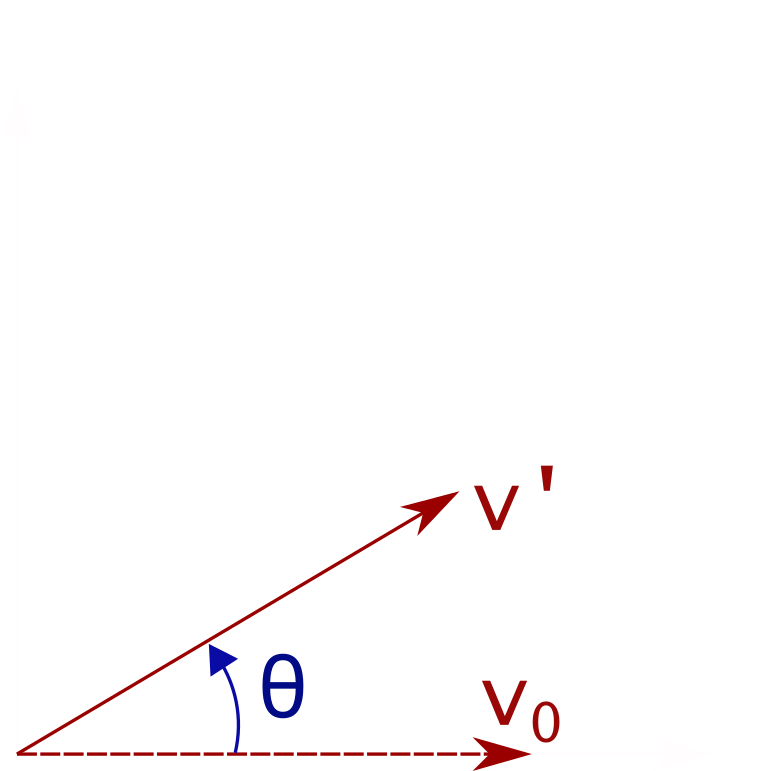
\includegraphics[width=0.35\textwidth]{img/RotationMatrix_1000}
            \caption{Rotating object}
            \label{fig:RotationMatrix_1000-png}
        \end{figure}

        In $\mathbb{R}^{2}$, consider the matrix that rotates a given
        vector $\mathbf{v}_{0}$ by a counterclockwise angle $\theta$ in
        a fixed coordinate system. Then

        \begin{equation}
            \mathbf{T}_{\theta} = \begin{bmatrix}
                \cos \theta & -\sin \theta \\
                \sin \theta & \cos \theta
            \end{bmatrix}
        ,\end{equation}

        so

        \begin{equation}
            \mathbf{v}^{'} = \mathbf{T}_{\theta}\mathbf{v}_{0}
        .\end{equation}

        \begin{figure}[ht]
            \centering
            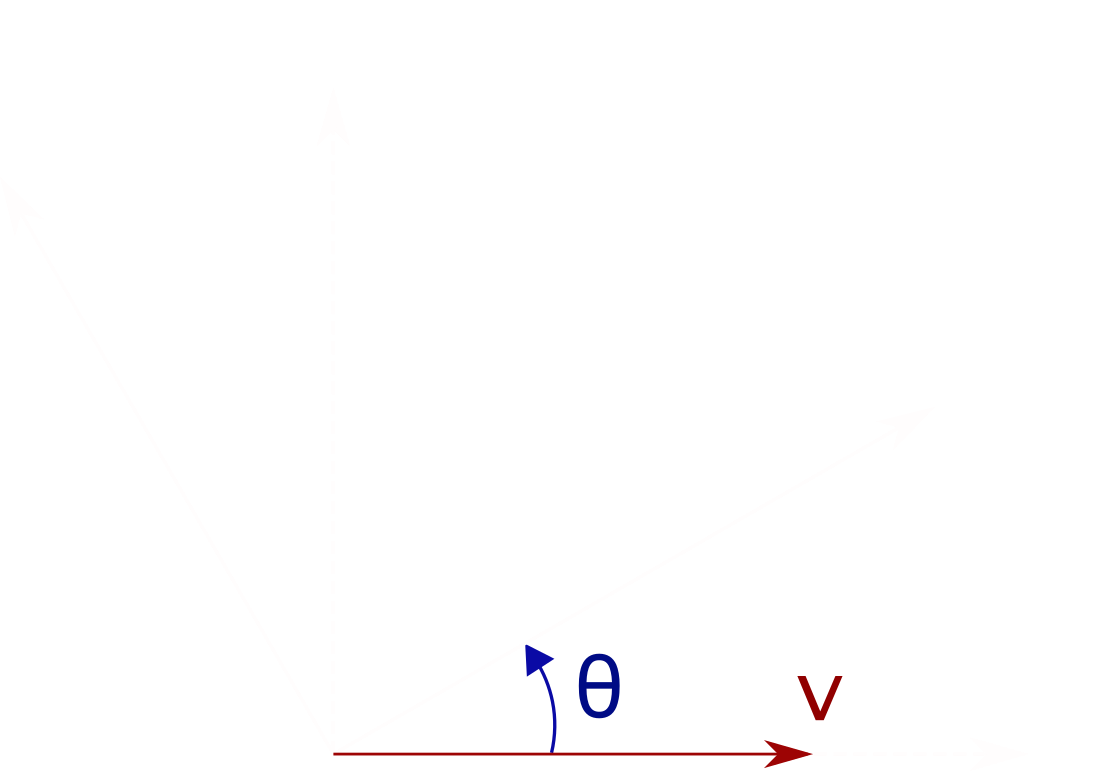
\includegraphics[width=0.5\textwidth]{img/RotationMatrixAxes_1000}
            \caption{Rotating Axes}
            \label{fig:RotationMatrixAxes_1000-png}
        \end{figure}

        On the other hand, consider the matrix that rotates the
        \textit{coordinate system} through a counterclockwise angle $\theta$.
        The coordinates of the fixed vector $\mathbf{v}$ in the rotated
        coordinate system are now given by a rotation matrix which is the
        \textit{transpose} of the fixed-axis matrix, as can be seen on the
        second figure, is equivalent to rotating the vector by
        a counterclockwise angle $-\theta$ relative to a fixed set of axes,
        giving:

        \begin{equation}
            \mathbf{T}_{\theta}^{'} = \begin{bmatrix}
                \cos \theta & \sin \theta \\
                -\sin \theta & \cos \theta
            \end{bmatrix}
        .\end{equation}

        This is the convention commonly used in textbooks.

    \item 3-D ($\mathbb{R}^{3}$):

        In $\mathbb{R}^{3}$, coordinate system rotations of the
        \textit{x-}, \textit{y-} and \textit{z-axis} in a counterclockwise
        direction when looking towards the origin give the matrices:

        \begin{equation}
            \mathbf{R}_{x}(\varphi) =
            \begin{bmatrix}
                1 & 0 & 0 \\
                0 & \cos \varphi & \sin \varphi \\
                0 & -\sin \varphi & \cos \varphi
            \end{bmatrix}
        .\end{equation}

        \begin{equation}
            \mathbf{R}_{y}(\theta) =
            \begin{bmatrix}
                \cos \theta & 0 & -\sin \theta \\
                0 & 1 & 0 \\
                \sin \theta & 0 & \cos \theta
            \end{bmatrix}
        .\end{equation}

        \begin{equation}
            \mathbf{R}_{z}(\psi) =
            \begin{bmatrix}
                \cos \psi & \sin \psi & 0 \\
                -\sin \psi & \cos \psi & 0 \\
                0 & 0 & 1
            \end{bmatrix}
        .\end{equation}

        Any \textbf{rotation} can be given as a composition of rotations
        about three axes (\textbf{Euler's rotation theorem}), and thus
        be represented by a $3 \times 3$ matrix operating on a vector.

        \begin{equation}
            \begin{bmatrix}
                x_{1}^{'} \\ x_{2}^{'} \\ x_{3}^{'}
            \end{bmatrix}
            =
            \begin{bmatrix}
                t_{11} & t_{12} & t_{13} \\
                t_{21} & t_{22} & t_{23} \\
                t_{31} & t_{32} & t_{33}
            \end{bmatrix}
            \begin{bmatrix}
                x_{1} \\ x_{2} \\ x_{3}
            \end{bmatrix}
        .\end{equation}

    \item \textbf{Euler's angles of XYZ rotation:}

        With the order of \textit{xyz} rotation the rotation matrix is
        composed as:

        \begin{equation}
            \scalebox{0.85}{
                $ \begin{array}{ll}
                    \mathbf{T}
                    &= \mathbf{R}_{z}(\psi)\mathbf{R}_{y}(\theta)\mathbf{R}_{x}(\varphi) \\
                    &=
                    \begin{bmatrix}
                        \cos \psi & \sin \psi & 0 \\
                        -\sin \psi & \cos \psi & 0 \\
                        0 & 0 & 1
                    \end{bmatrix}
                    \begin{bmatrix}
                        \cos \theta & 0 & -\sin \theta \\
                        0 & 1 & 0 \\
                        \sin \theta & 0 & \cos \theta
                    \end{bmatrix}
                    \begin{bmatrix}
                        1 & 0 & 0 \\
                        0 & \cos \varphi & \sin \varphi \\
                        0 & -\sin \varphi & \cos \varphi
                    \end{bmatrix} \\
                    &=
                    \begin{bmatrix}
                        \cos \theta \cos \psi
                        & \cos \psi \sin \theta \sin \varphi - \cos \varphi \sin \psi
                        & \cos \varphi \cos \psi \sin \theta + \sin \varphi \sin \psi \\
                        \cos \theta \sin \psi
                        & \cos \varphi \cos \psi + \sin \theta \sin \varphi \sin \psi
                        & \cos \varphi \sin \theta \sin \psi - \cos \psi \sin \varphi \\
                        -\sin \theta
                        & \cos \theta \sin \varphi
                        & \cos \theta \cos \varphi
                    \end{bmatrix}
                \end{array} $
            }
        \end{equation}

        Then the three \textit{Euler angles} for a \textit{xyz} rotation
        can be obtained:

        \begin{equation}
            \varphi = \atantwo(t_{32}, t_{33})
        ,\end{equation}

        \begin{equation}
            \theta = \atantwo \left(-t_{31}, \sqrt{ t_{32}^{2} + t_{33}^{2}} \right)
        ,\end{equation}

        \begin{equation}
            \psi = \atantwo(t_{21}, t_{11})
        ,\end{equation}

        where $\atantwo(y, x)$ definition is:

        \begin{equation}
            \atantwo(y, x) = \left\{
                \begin{array}{ll}
                    \arctan\left(\frac{y}{x}\right) & if \quad (x > 0),\\
                    \arctan\left(\frac{y}{x}\right) + \pi & if \quad (x < 0) \land (y \ge 0),\\
                    \arctan\left(\frac{y}{x}\right) - \pi & if \quad (x < 0) \land  (y < 0),\\
                    \frac{\pi}{2} & if \quad (x = 0) \land  (y > 0),\\
                    -\frac{\pi}{2} & if \quad (x = 0) \land  (y < 0),\\
                    undefined & if \quad (x = 0) \land (y = 0)
                \end{array}
            \right\}
        .\end{equation}

        \textbf{Note} the angle limitation for values returned while doing
        an Euler angle decomposition of a \textbf{rotation} matrix:

        \begin{equation}
            \begin{array}{l}
                \varphi \in (-\pi, \pi) \\
                \theta \in (-\frac{\pi}{2}, \frac{\pi}{2}) \\
                \psi \in (-\pi, \pi)
            \end{array}
        .\end{equation}

    \item Euler's angles of \textbf{ZYX} rotation:

        For a rotation defined in \textit{zyx} order the rotation matrix is:

        \begin{equation}
            \scalebox{0.85}{
                $ \begin{array}{ll}
                    \mathbf{T}
                    &= \mathbf{R}_{x}(\varphi)\mathbf{R}_{y}(\theta)\mathbf{R}_{z}(\psi) \\
                    &=
                    \begin{bmatrix}
                        1 & 0 & 0 \\
                        0 & \cos \varphi & \sin \varphi \\
                        0 & -\sin \varphi & \cos \varphi
                    \end{bmatrix}
                    \begin{bmatrix}
                        \cos \theta & 0 & -\sin \theta \\
                        0 & 1 & 0 \\
                        \sin \theta & 0 & \cos \theta
                    \end{bmatrix}
                    \begin{bmatrix}
                        \cos \psi & \sin \psi & 0 \\
                        -\sin \psi & \cos \psi & 0 \\
                        0 & 0 & 1
                    \end{bmatrix} \\
                    &=
                    \begin{bmatrix}
                        \cos \theta \cos \varphi
                        & - \cos \theta \sin \varphi
                        & \sin \varphi \\
                        \cos \psi \sin \varphi + \cos \varphi \sin \theta \sin \psi
                        & \cos \varphi \cos \psi - \sin \theta \sin \varphi \sin \psi
                        & -\cos \theta \sin \psi \\
                        \sin \varphi \sin \psi - \cos \varphi \cos \psi \sin \theta
                        & \cos \psi \sin \theta \sin \varphi + \cos \varphi \sin \psi
                        & \cos \theta \cos \psi
                    \end{bmatrix}
                \end{array} $
            }
        .\end{equation}

        \textbf{Note that the angles $\varphi$, $\theta$ and $\psi$ defined here are
        different from the \textit{XYZ} rotation defined above!} The rotation
        is performed by first rotating around \textit{z-axis} counterclockwise
        by an angle $\psi$, then around \textit{y-axis} counterclockwise
        by an angle $\theta$ and finaly around \textit{x-axis}, counterclockwise,
        by an angle $\varphi$.

        Then the \textit{Euler's angles} can be obtained as:

        \begin{equation}
            \left\{ \begin{array}{l}
                \varphi = \arctan \left( \frac{-t_{12}}{t_{11}} \right)\\
                \theta = \arcsin \left( t_{13} \right) \\
                \psi = \arctan \left( \frac{-t_{23}}{t_{33}} \right)
            \end{array} \right.
        .\end{equation}


    \item Alternate way of constructing \textbf{Rotation matrix} without specifying
        angles:

        The rotation matrix to a new coordinate system can be constructed from
        its axes, where the rotation matrix can be defined as:

        \begin{equation}
            \mathbf{T}_{R} = \begin{bmatrix}
                x_1 & x_2 & x_3 \\
                y_1 & y_2 & y_3 \\
                z_1 & z_2 & z_3 \\
            \end{bmatrix}
        ,\end{equation}

        where $\mathbf{x} = [x_1, x_2, x_3]^{T}$, $\mathbf{y} = [y_1, y_2, y_3]^{T}$
        and  $\mathbf{z} = [z_1, z_2, z_3]^{T}$ are unit vectors in the direction
        of \textit{x-}, \textit{y-} and \textit{z-axis} of the new coordinate
        system.


        \begin{bbox}[0.85]
            The \textbf{transformation matrix} can be defined by any two vectors
            $\mathbf{u}$ and $\mathbf{v}$, where $\mathbf{u}$ defines the direction
            of \textit{x-axis} and $\mathbf{v}$ defines the \textit{xy-plane}.
            To construct the \textbf{rotation matrix} use the following steps:

            \begin{enumerate}
                \item create x-axis of unit lenght

                    \begin{equation}
                        \mathbf{x} = \frac{\mathbf{u}}{||\mathbf{u}||}
                    .\end{equation}

                \item create z-axis of unit lenght

                    \begin{equation}
                        \mathbf{z}
                        = \frac{\mathbf{u} \times \mathbf{v}}{||\mathbf{u} \times \mathbf{v}||}
                    .\end{equation}

                \item create y-axis of unit lenght

                    \begin{equation}
                        \mathbf{y}
                        = \frac{\mathbf{z} \times \mathbf{x}}{||\mathbf{z} \times \mathbf{x}||}
                    .\end{equation}

                \item compose \textbf{rotation matrix}

                    \begin{equation}
                        \mathbf{T}_{R} = \begin{bmatrix}
                            \mathbf{x}^{T} \\
                            \mathbf{y}^{T} \\
                            \mathbf{z}^{T}
                        \end{bmatrix}
                    .\end{equation}
            \end{enumerate}

            The creation of the \textbf{rotation matrix} by any two other vectors is
            analogic, as \textbf{orthogonal} base must be constructed first, then
            the matrix is composed of its vectors.
        \end{bbox}

        \begin{bbox}[0.85]
            To test, whether the transformation matrix is correct, one can use
            the orthogonality criterion:

            \begin{equation}
                \mathbf{T}^{T} = \mathbf{T}^{-1}
            .\end{equation}

            \begin{equation}
                \mathbf{T}\mathbf{T}^{T} = \mathbf{T}^{T}\mathbf{T} = \mathbf{I}
            .\end{equation}

            or

            \begin{equation}
                \det(\mathbf{T}) = 1
            .\end{equation}
        \end{bbox}

\end{enumerate}


\section{Coordinate Transformation}

\begin{itemize}
    \item \textbf{Rotation:}

        Let $\mathbf{A}^{T} = [a_{x}, a_{y}, a_{z}]$ be the original coordinates,
        $\mathbf{B}^{T} = [b_{x}, b_{y}, b_{z}]$ be the transformed coordinates, and
        $\mathbf{T}$ a tranformation matrix in the form:

        \begin{equation}
            \mathbf{T} = \begin{bmatrix}
                x_1 & x_2 & x_3 \\
                y_1 & y_2 & y_3 \\
                z_1 & z_2 & z_3
            \end{bmatrix} = \begin{bmatrix}
                \mathbf{x} \\
                \mathbf{y} \\
                \mathbf{z}
            \end{bmatrix}
        ,\end{equation}

        where $\mathbf{x} = [x_1, x_2, x_3]$, $\mathbf{y} = [y_1, y_2, y_3]$ and
        $\mathbf{z} = [z_1, z_2, z_3]$ are the \textit{x-axis}, \textit{y-axis} and
        \textit{z-axis} \textbf{unit vectors}, respectively, of the new coordinate
        system defined in the original one, while sharing their origin.

        The following applies:

        \begin{equation}
            \mathbf{T} \times \mathbf{A} = \mathbf{B}
        ,\end{equation}

        and

        \begin{equation}
            \mathbf{T}^{T} \times \mathbf{B} = \mathbf{A}
        .\end{equation}

        \textbf{Note:} Perpendicular vector is  created using \textit{cross-product}.
\end{itemize}


\section{Tensor Transformation}

From:

\href{https://wp.optics.arizona.edu/optomech/wp-content/uploads/sites/53/2016/10/OPTI_222_W21.pdf}{source 1},
\href{https://www.continuummechanics.org/principalstressesandstrains.html}{source 2},
\href{https://www.ecourses.ou.edu/cgi-bin/eBook.cgi?doc=&topic=me&chap_sec=07.2&page=theory}{source 3}

Let real symmetric matrix  $\mathbf{A}$ be the original tensor,
real symmetric matrix $\mathbf{B}$ the transformed tensor, and
orthogonal matrix $\mathbf{T}$ a tranformation matrix in the form:

\begin{equation}
    \mathbf{A} = \begin{bmatrix}
        \sigma^{A}_{11} & \sigma^{A}_{12} & \sigma^{A}_{13} \\
        \sigma^{A}_{21} & \sigma^{A}_{22} & \sigma^{A}_{23} \\
        \sigma^{A}_{31} & \sigma^{A}_{32} & \sigma^{A}_{33}
    \end{bmatrix}
,\end{equation}

\begin{equation}
    \mathbf{B} = \begin{bmatrix}
        \sigma^{B}_{11} & \sigma^{B}_{12} & \sigma^{B}_{13} \\
        \sigma^{B}_{21} & \sigma^{B}_{22} & \sigma^{B}_{23} \\
        \sigma^{B}_{31} & \sigma^{B}_{32} & \sigma^{B}_{33}
    \end{bmatrix}
,\end{equation}

\begin{equation}
    \mathbf{T} = \begin{bmatrix}
        x_1 & x_2 & x_3 \\
        y_1 & y_2 & y_3 \\
        z_1 & z_2 & z_3
    \end{bmatrix} = \begin{bmatrix}
        \mathbf{x} \\
        \mathbf{y} \\
        \mathbf{z}
    \end{bmatrix}
,\end{equation}

where $\mathbf{x} = [x_1, x_2, x_3]$, $\mathbf{y} = [y_1, y_2, y_3]$ and
$\mathbf{z} = [z_1, z_2, z_3]$ are the \textit{x-axis}, \textit{y-axis} and
\textit{z-axis} \textbf{unit vectors}, respectively, of the new coordinate
system defined in the original one, while sharing their origin.

The transformation matrix $\mathbf{T}$ must satisfy
$\mathbf{T}\mathbf{T}^{T} = \mathbf{T}^{T}\mathbf{T} = \mathbf{I}$, where $\mathbf{I}$
is an identity matrix. This means that transformation matrix must be orthogonal,
therefore satisfying $\mathbf{T}^{T} = \mathbf{T}^{-1}$.

Then \textbf{tensor transformation} is performed as such:

\begin{equation}
    \mathbf{T} \times \mathbf{A} \times \mathbf{T}^{T} = \mathbf{B}
.\end{equation}

\begin{equation}
    \mathbf{T}^{T} \times \mathbf{B} \times \mathbf{T} = \mathbf{A}
.\end{equation}

\begin{itemize}
    \item \textbf{Principal values:}

        The principal values can be found as the \textbf{eigenvalues} of the tensor
        matrix.

        Characteristic equation of tensor $\mathbf{\Sigma}$:

        \begin{equation}
            \mathbf{\Sigma}\mathbf{V} = \mathbf{\Lambda} \mathbf{V}
        ,\end{equation}

        therefore:

        \begin{equation}
            (\mathbf{\Sigma} - \mathbf{\Lambda}\mathbf{I})\mathbf{V} = 0
        ,\end{equation}

        and:

        \begin{equation}
            det(\mathbf{\Sigma} - \mathbf{\Lambda}\mathbf{I}) = 0
        ,\end{equation}

        where $\mathbf{\Lambda}$ is a diagonal matrix of eigenvalues (principal values)
        and $\mathbf{V}$ is the eigenvector matrix.

        The characteristic cubic equation can be also written as:

        \begin{equation}
            \lambda^{3} - I_{1}\lambda^{2} + I_{2}\lambda - I_{3} = 0
        ,\end{equation}

        giving three roots equal to tensor eigenvalues.

        First compute \textbf{Invariants} $\mathbf{I}_{n}$:

        \begin{equation}
            \begin{array}{ll}
                I_{1} &= \sigma_{11} + \sigma_{22} + \sigma_{33} \\
                I_{2} &= \sigma_{11}\sigma_{22} + \sigma_{22}\sigma_{33}
                + \sigma_{33}\sigma_{11} - \sigma_{12}^{2} - \sigma_{13}^{2} - \sigma_{23}^{2} \\
                I_{3}
                &= \sigma_{11}\sigma_{22}\sigma_{33}
                - \sigma_{11}\sigma_{23}^{2}
                - \sigma_{22}\sigma_{13}^{2}
                - \sigma_{33}\sigma_{12}^{2}
                + 2 \sigma_{12}\sigma_{13}\sigma_{23}
            \end{array}
        .\end{equation}

        In matrix form:

        \begin{equation}
            \begin{array}{ll}
                I_{1} &= tr[\mathbf{\Sigma}] \\
                I_{2} &= \left| \begin{matrix}
                    \sigma_{11} & \sigma_{12} \\
                    \sigma_{12} & \sigma_{22}
                \end{matrix} \right| + \left| \begin{matrix}
                    \sigma_{11} & \sigma_{13} \\
                    \sigma_{13} & \sigma_{33}
                \end{matrix} \right| + \left| \begin{matrix}
                    \sigma_{22} & \sigma_{23} \\
                    \sigma_{23} & \sigma_{33}
                \end{matrix} \right| \\
                    I_{3} &= det(\mathbf{\Sigma})
            \end{array}
        .\end{equation}

        Then compute \textit{help values}:

        \begin{equation}
            Q = \frac{3 I_{2} - I_{1}^{2}}{9}
        ,\end{equation}

        \begin{equation}
            R = \frac{2 I_{1}^{3} - 9 I_{1} I_{2} + 27 I_{3}}{54} \\
        ,\end{equation}

        \begin{equation}
            \theta = cos^{-1} \left( \frac{ R }{ \sqrt{- Q^{3}}} \right)
        .\end{equation}

        Lastly to get \textbf{principal values}:

        \begin{equation}
            \overline{\sigma_{1}}
            = 2 \sqrt{-Q} \cos{\left(\frac{\theta}{3}\right)} + \frac{1}{3}I_{1}
        .\end{equation}

        \begin{equation}
            \overline{\sigma_{2}}
            = 2 \sqrt{-Q} \cos{\left(\frac{\theta + 2 \pi}{3}\right)} + \frac{1}{3}I_{1}
        .\end{equation}

        \begin{equation}
            \overline{\sigma_{3}}
            = 2 \sqrt{-Q} \cos{\left(\frac{\theta + 4 \pi}{3}\right)} + \frac{1}{3}I_{1}
        .\end{equation}

        The \textbf{principal values are not sorted}. The principal tensor is then:

        \begin{equation}
            \mathbf{\Sigma} = \begin{bmatrix}
                \sigma_{1} & 0 & 0 \\
                0 & \sigma_{2}  & 0 \\
                0 & 0 & \sigma_{3}
            \end{bmatrix}
        ,\end{equation}

        where $\overline{\sigma}_{1}$, $\overline{\sigma}_{2}$ and $\overline{\sigma}_{3}$
        $\implies$ $\sigma_1 > \sigma_2 > \sigma_3$.

        Afterwards the \textbf{principal axes} are obtained as:

        \begin{equation}
            \begin{array}{l}
                \mathbf{\Gamma}_{1} = \mathbf{\Sigma} - \sigma_{1}\mathbf{I} \\
                \mathbf{\Gamma}_{2} = \mathbf{\Sigma} - \sigma_{2}\mathbf{I} \\
                \mathbf{\Gamma}_{3} = \mathbf{\Sigma} - \sigma_{3}\mathbf{I}
            \end{array}
        ,\end{equation}

        where $\mathbf{\Gamma}$ is a coordinate system corresponding to the
        principal value \textit{i} and $\mathbf{I}$ is a $3 \times 3$
        identity matrix.

        The vectors corresponding to each \textbf{principal value} are obtained:

        \begin{equation}
            \mathbf{\Gamma}_{1}
            = \begin{bmatrix}
                \overline{x}_{11} & \overline{x}_{12} & \overline{x}_{13}\\
                \overline{y}_{11} & \overline{y}_{12} & \overline{y}_{13}\\
                \overline{z}_{11} & \overline{z}_{12} & \overline{z}_{13}
            \end{bmatrix}
            = \begin{bmatrix}
                \overline{\mathbf{x}}_{1}\\
                \overline{\mathbf{y}}_{1}\\
                \overline{\mathbf{z}}_{1}
            \end{bmatrix}
        ,\end{equation}
        \begin{equation}
            \mathbf{\Gamma}_{2}
            = \begin{bmatrix}
                \overline{x}_{21} & \overline{x}_{22} & \overline{x}_{23}\\
                \overline{y}_{21} & \overline{y}_{22} & \overline{y}_{23}\\
                \overline{z}_{21} & \overline{z}_{22} & \overline{z}_{23}
            \end{bmatrix}
            = \begin{bmatrix}
                \overline{\mathbf{x}}_{2}\\
                \overline{\mathbf{y}}_{2}\\
                \overline{\mathbf{z}}_{2}
            \end{bmatrix} \\
        ,\end{equation}
        \begin{equation}
            \mathbf{\Gamma}_{3}
            = \begin{bmatrix}
                \overline{x}_{31} & \overline{x}_{32} & \overline{x}_{33}\\
                \overline{y}_{31} & \overline{y}_{32} & \overline{y}_{33}\\
                \overline{z}_{31} & \overline{z}_{32} & \overline{z}_{33}
            \end{bmatrix}
            = \begin{bmatrix}
                \overline{\mathbf{x}}_{3}\\
                \overline{\mathbf{y}}_{3}\\
                \overline{\mathbf{z}}_{3}
            \end{bmatrix}
        ,\end{equation}

        where $\overline{\mathbf{x}}$, $\overline{\mathbf{y}}$ and $\overline{\mathbf{z}}$ are vectors of size 3.

        \begin{equation}
              \mathbf{x} = \frac{\overline{\mathbf{y}}_{1} \times \overline{\mathbf{z}}_{1}}
              {|\overline{\mathbf{y}}_{1} \times \overline{\mathbf{z}}_{1}|}\\
        ,\end{equation}
        \begin{equation}
              \mathbf{y} = \frac{\overline{\mathbf{z}}_{2} \times \overline{\mathbf{x}}_{2}}
              {|\overline{\mathbf{z}}_{2} \times \overline{\mathbf{x}}_{2}|}\\
        ,\end{equation}
        \begin{equation}
              \mathbf{z} = \frac{\overline{\mathbf{x}}_{3} \times \overline{\mathbf{y}}_{3}}
              {|\overline{\mathbf{x}}_{3} \times \overline{\mathbf{y}}_{3}|}
        .\end{equation}

        The principal axes are also the \textbf{eigenvectors} of tensor $\mathbf{\Sigma}$:

        \begin{equation}
            \mathbf{V} = \begin{bmatrix}
                \mathbf{x} & \mathbf{y} & \mathbf{z}
            \end{bmatrix} = \begin{bmatrix}
                x_1 & y_1 & z_1 \\
                x_2 & y_2 & z_2 \\
                x_3 & y_3 & z_3
            \end{bmatrix}
        .\end{equation}

    \item \textbf{Maximum Shear value:}


        Maximum \textbf{shear stress} occurs at an angle of 45 degrees to principal axes.
        If principal stresses are aligned such that $\sigma_1 > \sigma_2 > \sigma_3$
        and the stress tensor is:

        \begin{equation}
            \mathbf{\Sigma} = \begin{bmatrix}
                \sigma_1 & 0 & 0 \\
                0 & \sigma_2 & 0 \\
                0 & 0 & \sigma_3
            \end{bmatrix}
        ,\end{equation}

        then maximum shear stress $\tau_{max}$ can be obtained as follows:

        \begin{equation}
            \tau_{max} = \frac{\sigma_1 - \sigma_3}{2}
        \end{equation}

        and is at 45 degrees angle in the 1-3 plane of the principal axes to the
        principal coordinate system.

        More generally (in 2D):

        \begin{equation}
            \tau_{max} = \sqrt{\left(\frac{\sigma_{x} - \sigma_{y}}{2}\right)^{2}
            + \tau_{xy}^{2}}
        .\end{equation}

        \begin{bbox}[0.85]
            When the principal tensor is rotated by 45 degrees to obtain \textbf{maximum
            shear stress}, the axial stress components corresponding to this shear
            stress are equal.

            The value of maximal shear stress is obtained:

            \begin{equation}
                \tau_{max} = \frac{\sigma_{max} - \sigma_{min}}{2}
            .\end{equation}

            The value of axial stresses corresponding to maximal shear stress is
            the average of maximal and minimal axial stresses:

            \begin{equation}
                \sigma_{\tau_{max}} = \frac{\sigma_{max} + \sigma_{min}}{2}
            .\end{equation}

        \end{bbox}

    \item \textbf{Example:}

        Let a stress tensor in principal coordinate system be:

        \begin{equation}
             \mathbf{\Sigma} = \begin{bmatrix}
                 433 & 0 & 0 \\
                 0 & 125 & 0 \\
                 0 & 0 & 24
             \end{bmatrix}
        ,\end{equation}

        then $\sigma_1 = \sigma_{max} = 433 \text{ MPa}$ and
        $\sigma_3 = \sigma_{min} = 24 \text{ MPa}$.

        Transformation matrix for rotating by 45 degrees in 3-1 plane is:

        \begin{equation}
            \mathbf{T} = \begin{bmatrix}
                \frac{\sqrt{2}}{2} & 0 & -\frac{\sqrt{2}}{2} \\
                0 & 1 & 0 \\
                \frac{\sqrt{2}}{2} & 0 & \frac{\sqrt{2}}{2}
            \end{bmatrix}
        .\end{equation}

        Rotating tensor $\mathbf{\Sigma}$ by transformation matrix $\mathbf{T}$ we get:

        \begin{equation}
            \mathbf{\Sigma}_{\tau} = \mathbf{T}\mathbf{\Sigma}\mathbf{T}^{T}
            = \begin{bmatrix}
                228.5 & 0 & 204.5 \\
                0 & 125 & 0 \\
                204.5 & 0 & 228.5
            \end{bmatrix}
        ,\end{equation}

        where:

        \begin{equation}
            \begin{array}{l}
                \tau_{max} = \sigma_{13} = \sigma_{31} = 204.5 \\
                \sigma_{11} = \sigma_{33} = 228.5 \\
                \sigma_{22} = \sigma_2
            \end{array}
        .\end{equation}

        Check for correct values:

        \begin{equation}
            \tau_{max} = \frac{\sigma_1 - \sigma_3}{2} = \frac{433 - 24}{2}
            = \frac{409}{2} = 204.5 \text{ MPa} \implies \text{OK!}
        ,\end{equation}

        \begin{equation}
            \sigma_{11} = \sigma_{33} = \frac{\sigma_1 + \sigma_3}{2}
            = \frac{433 + 24}{2} = 228.5 \text{ MPa} \implies \text{OK!}
        .\end{equation}

        \textbf{$\sigma_2$ has not changed as it is colinear with the axis of rotation.}

        The relationship between principal normal streses and maximum shear stresses
        can be better understood by examining a plot of the stresses as a function
        of the rotation angle.

        Notice that there are multiple $\theta_{p}$ and $\theta_{\tau - max}$
        angles because of the periodical nature of the equations. However, they
        will give the same absolute values.

        At the principal stress angle, $\theta_{p}$, the shear stress will always be zero,
        as shown on the diagram. And the maximum shear stress will occur when the
        two principal normal stresses, $\sigma_1$ and $\sigma_2$, are equal.

        \begin{figure}[ht]
            \centering
            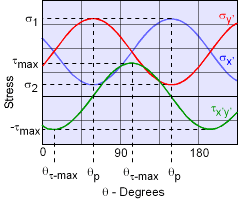
\includegraphics[width=0.8\textwidth]{img/stresses_as_function_of_angle}
            \caption{Stresses as a function of angle}
            \label{fig:stresses_as_function_of_angle-png}
        \end{figure}

        \begin{bbox}[0.85]
            When $\sigma_{x}$ or $\sigma_{y}$ are either max or min, the shear stress
            $\tau_{xy}$ is equal to 0. When shear stress $\tau_{xy}$ is max or min,
            the stresses $\sigma_{x}$ and $\sigma_{y}$ are equal to their average.
        \end{bbox}


\end{itemize}


\section{Moment of Inertia}

From: \href{https://en.wikipedia.org/wiki/Parallel_axis_theorem}{Parallel axis theorem}

\textit{Parallel axis theorem}, also known as \textit{Huygens-Steiner's theorem}
or just \textit{Steiner's theorem} can be used to determine the \textbf{moment of inertia}
or \textbf{second moment of area} of a rigid body about any axis, given the body's
moment of inertia about a parallel axis through the objects center of gravity
and the perpendicular distance between the axes.

Moment of Inertia = \textbf{tensor}.

\begin{itemize}
    \item \textbf{Steiner's share:}

        \begin{equation}
            \mathbf{I}_{ss} = m \times \begin{bmatrix}
                y^{2} + z^{2} & -xy & -xz \\
                -yz & x^{2} + z^{2} & -yz \\
                -zx & -zy & x^{2} + y^{2}
            \end{bmatrix}
        .\end{equation}

        \textbf{Identities for a skew-symmetric matrix}

        In order to compare formulations of the parallel axis theorem using
        skew-symmetric matrices and the tensor formulation, the following
        identities are useful.

        Let $[\mathbf{R}]$ be the skew-symmetric matrix associated with the
        position vector $\mathbf{R} = (x, y, z)$, then the product in
        the inertia matrix becomes:

        \begin{equation}
            -[\mathbf{R}][\mathbf{R}] = \begin{bmatrix}
                0 & -z & y \\
                z & 0 & -x \\
                -y & x & 0
            \end{bmatrix}^{2}
            = \begin{bmatrix}
                y^{2} + z^{2} & -xy & -xz \\
                -yz & x^{2} + z^{2} & -yz \\
                -zx & -zy & x^{2} + y^{2}
            \end{bmatrix}
        .\end{equation}

        This product can be computed using the matrix formed by the outer product
        $[\mathbf{R} \mathbf{R}^{T}]$ using the identity

        \begin{equation}
            \begin{array}{ll}
                 \\
                -[\mathbf{R}]^{2}
                &= |\mathbf{R}|^{2}|\mathbf{E}_{3}| - [\mathbf{R}\mathbf{R}^{T}] \\
                &= \begin{bmatrix}
                    x^{2} + y^{2} + z^{2} & 0 & 0 \\
                    0 & x^{2} + y^{2} + z^{2} & 0 \\
                    0 & 0 & 0
                \end{bmatrix} - \begin{bmatrix}
                    x^{2} & xy & xz \\
                    yx & y^{2} & yz \\
                    zx & zy & z^{2}
                \end{bmatrix}
            \end{array}
        ,\end{equation}

        where $[\mathbf{E}_{3}$ is the $n \times n$  identity matrix.

        Also notice, that

        \begin{equation}
            |\mathbf{R}|^{2} = \mathbf{R} \cdot \mathbf{R} = tr [\mathbf{R}\mathbf{R}^{T}]
        .\end{equation}

        where $tr$ denotes the sum of the diagonal elements of the outer product
        matrix, known as its \textit{trace}.

        To obtain matrix of moments of inertia by rotating about any random
        point $A$ while having the moment of inertia in the center of gravity of
        the object $\mathbf{I}_{COG}$ and the coordinate distance $d = [x, y, z]$
        between the point $A$ and \textbf{COG} we:

        \begin{enumerate}
            \item Compute the moment of inertia relative to point $A$

                 \begin{equation}
                    \mathbf{I}_{A} = \mathbf{I}_{COG} + m \times \mathbf{I}_{SS}^{A \to COG}
                .\end{equation}

            \item Transform the tensor $\mathbf{I}_{A}$ to new rotated coordinate
                system using transformation matrix $\mathbf{T}$:

                \begin{equation}
                    \mathbf{I}_{A}^{'} = \mathbf{T} \times \mathbf{I}_{A} \times \mathbf{T}^{T}
                .\end{equation}

            \item Subtract the \textbf{Steiner's share} relative to new \textbf{COG}

                \begin{equation}
                    \mathbf{I}_{COG}^{'} = \mathbf{I}_{A}^{'} - \mathbf{I}_{SS}^{A' \to COG'}
                .\end{equation}

        \end{enumerate}



\end{itemize}


\newpage
\chapter{Boundary conditions not in GCS}

\section{Skew boundary conditions}
\textit{Skew boundary conditions}, also known as \textbf{Rotated BCs} are implemented
after assembling the global stiffness matrix $ \m{K} $.

Basic equation:

\begin{equation}
    \m{M} \ddot{\m{u}} + \m{C} \dot{\m{u}} + \m{K} \m{u}
    = \m{f}
\end{equation}

First we need to identify all prescribed BCs that do not correspond to the
defined assemblage DOFs and transform the finite equilibrium equations to
correspond to the prescribed BCs. Thus we write:

\begin{equation}\label{skew-bcs}
    \m{u} = \m{T} \closure{\m{u}}
\end{equation}

where $ \closure{\m{u}} $ is the vector of nodal point DOFs in the required
directions. The transformation matrix $ \m{T} $ is an identity matrix
that has been altered by the directional sines and cosines of the components
$ \closure{\m{u}} $ measured in the original displacement directions.
Using \eqref{skew-bcs}, we obtain:

\begin{equation}
    \closure{\m{M}} \closure{\ddot{\m{u}}}
    + \closure{\m{C}} \closure{\dot{\m{u}}}
    + \closure{\m{K}} \closure{\m{u}}
    = \closure{\m{f}}
\end{equation}

where:

\begin{eqarray}\label{skew-eq-of-motion}
    \closure{\m{M}} & = \m{T}^T \m{M} \m{T} \\
    \closure{\m{C}} & = \m{T}^T \m{C} \m{T} \\
    \closure{\m{K}} & = \m{T}^T \m{K} \m{T} \\
    \closure{\m{f}} & = \m{T}^T \m{f}
\end{eqarray}

We should note that the matrix multiplications in \eqref{skew-eq-of-motion}
involve changes only in those columns and rows of $ \m{M} $, $ \m{C} $,
$ \m{K} $ and $ \m{f} $ that are actually affected. In practice,
the transformation is carried out effectively on the element level just prior
to adding the element matrices to the global matrices.


\newpage
\section{Cartesian CSYS}

When a node or an SPC is defined as a \textbf{rotated}/\textbf{skewed} or in
a different type of Coordinate system (e.g. cylindrical) a transformation matrix
needs to be applied to such nodes.

\textbf{Cartesian Coordinate system} definition by angle (2D):
\begin{equation}
    \m{u}_l = \m{T} \m{u}_g
\end{equation}

Unpacked:
\begin{equation}
    \begin{bmatrix}
        u_l \\
        w_l \\
        \psi_l \\
    \end{bmatrix}
    = \begin{bmatrix}
        \phantom{-}\cos \alpha & \sin \alpha & 0 \\
        -\sin \alpha & \cos \alpha & 0 \\
        0 & 0 & 1 \\
    \end{bmatrix}
    \begin{bmatrix}
        u_g \\
        w_g \\
        \psi_g \\
    \end{bmatrix}
\end{equation}

%TODO: \textbf{Cartesian Coordinate system} definition by angle (3D):


\textbf{Cartesian Coordinate system} definition by vectors (3D):

when a \textbf{CSYS} is defined by an \textbf{origin} and \textbf{two vectors}
$ \m{x} = \begin{pmatrix} x_1 & x_2 & x_3 \end{pmatrix} $
and $ \m{y} = \begin{pmatrix} y_1 & y_2 & y_3 \end{pmatrix} $,
then for a Cartesian CSYS it suffices to:
\begin{eqarray}
    \m{\closure{x}} &= \frac{\m{x}}{||\m{x}||} \\
    \m{\closure{y}} &= \frac{\m{y}}{||\m{y}||} \\
    \m{\closure{z}} &= \m{\closure{x}} \times \m{\closure{y}} \\
\end{eqarray}

The transformation relation:
\begin{equation}
    \m{u}_l = \m{T} \m{u}_g
\end{equation}

when unpacked:
\begin{equation}
    \begin{bmatrix}
        u_l \\
        v_l \\
        w_l \\
        \phi_l \\
        \psi_l \\
        \rho_l \\
    \end{bmatrix}
    = \begin{bmatrix}
        \m{x} & \m{0} \\
        \m{y} & \m{0} \\
        \m{z} & \m{0} \\
        \m{0} & \m{x} \\
        \m{0} & \m{y} \\
        \m{0} & \m{z} \\
    \end{bmatrix}
    \begin{bmatrix}
        u_g \\
        v_g \\
        w_g \\
        \phi_g \\
        \psi_g \\
        \rho_g \\
    \end{bmatrix}
\end{equation}

Where $ \m{0} $ is a $ 3 \times 1 $ zero vector.

For a \textbf{2D case} just \textbf{one vector} is enough, the
$ \m{\closure{z}} = \begin{pmatrix} 0 & 0 & 1 \end{pmatrix} $ and following relations
apply:
\begin{eqarray}
    \m{\closure{x}} &= \m{\closure{y}} \times \m{\closure{z}} \\
    \m{\closure{y}} &= \m{\closure{z}} \times \m{\closure{x}} \\
    \m{\closure{z}} &= \m{\closure{x}} \times \m{\closure{y}} \\
\end{eqarray}

This means that a \textbf{CSYS} defined by an \textbf{origin} point
$ \m{O} = \begin{pmatrix} x_O & y_O & z_O \end{pmatrix} $,
point laying on \textbf{x axis}
$ \m{P}_x = \begin{pmatrix} x_{P_x} & y_{P_x} & z_{P_x} \end{pmatrix} $ and a
point laying in \textbf{xy plane}
$ \m{P}_{xy} = \begin{pmatrix} x_{P_{xy}} & y_{P_{xy}} & z_{P_{xy}} \end{pmatrix} $
define a CSYS followingly:
\begin{eqarray}
    \m{x} &= \begin{pmatrix} x_{P_x} - x_O & y_{P_x} - y_O & z_{P_x} - z_O \end{pmatrix} \\
    \m{\closure{x}} &= \frac{\m{x}}{||\m{x}||} \\
    \m{\hat{y}} &= \begin{pmatrix} x_{P_{xy}} - x_O & y_{P_{xy}} - y_O & z_{P_{xy}} - z_O \end{pmatrix} \\
    \m{\closure{\hat{y}}} &= \frac{\m{\hat{y}}}{||\m{\hat{y}}||} \\
    \m{\closure{z}} &= \m{\closure{x}} \times \m{\closure{\hat{y}}} \\
    \m{\closure{y}} &= \m{\closure{z}} \times \m{\closure{x}} \\
\end{eqarray}


\newpage
\section{Cylidrical CSYS}

The basic relation between a point in \textbf{cartesian} and \textbf{cylindrical}
CSYS is (when the cartesian CSYS has the same origin as the cylindrical one
and both CSYS $ z $ axes overlay):
\begin{eqarray}
    x &= r \cos \varphi \\
    y &= r \sin \varphi \\
    z &= z \\
\end{eqarray}

 in one direction and:
 \begin{eqarray}
     r &= \sqrt{x^2 + y^2} \\
     \varphi &= \left\{ \begin{array}{cc}
                indeterminate & if\ x = 0\ and\ y = 0 \\
                \arcsin \frac{y}{r} & if\ x \ge 0 \\
                -\arcsin \frac{y}{r} + \pi & if\ x < 0\ and\ y \ge 0 \\
                -\arcsin \frac{y}{r} + \pi & if\ x < 0\ and\ y < 0 \\
             \end{array} \right.
 \end{eqarray}

 in the other. One can also use the $ \arctan $ function to compute $ \varphi $:
 \begin{equation}
     \varphi = \left\{ \begin{array}{cc}
             indeterminate & if\ x = 0\ and\ y = 0 \\
             \frac{\pi}{2}\frac{y}{|y|} & if\ x = 0\ and\ y \ne 0 \\
             \arctan \frac{y}{x} & if\ x > 0 \\
             \arctan \frac{y}{x} + \pi & if\ x < 0\ and\ y \ge 0 \\
             \arctan \frac{y}{x} - \pi & if\ x < 0\ and\ y < 0 \\
         \end{array} \right.
 \end{equation}

 This is also called the $ \atantwo (y, x) $ function!

 To transform node coordinates from \textbf{cartesian} to \textbf{cylindrical},
 three transforms are in order:

 \begin{enumerate}
     \item translate the coordinates so that \textbf{origin} of the new
         CSYS conforms to the \textbf{origin} of the \textbf{cylidrical}
         CSYS.

         \begin{equation}
             \m{x}_1 = \m{T}_T \m{x}_0
         \end{equation}

         \begin{equation}
             \begin{bmatrix}
                 x_1 \\
                 y_1 \\
                 z_1 \\
                 1 \\
             \end{bmatrix}
             = \begin{bmatrix}
                 1 & 0 & 0 & -x_O^c \\
                 0 & 1 & 0 & -y_O^c \\
                 0 & 0 & 1 & -z_O^c \\
                 0 & 0 & 0 & \phantom{-}1 \\
             \end{bmatrix}
             \begin{bmatrix}
                 x_0 \\
                 y_0 \\
                 z_0 \\
                 1 \\
             \end{bmatrix}
         \end{equation}

         where $ \m{x}_O^c $ denotes the \textbf{cylindrical} CSYS origin
         and $ \m{T}_T $ denotes the translation matrix.

    \item \textbf{rotate} the node to a new \textbf{cartesian} CSYS so that
        the new CSYS \textbf{x-axis} conforms to the cylindrical CSYS
        \textbf{r-axis} and the new CSYS \textbf{z-axis} conforms to the
        cylindrical \textbf{z-axis}.

        \begin{equation}
            \m{x}_2 = \m{T}_R \m{x}_1
        \end{equation}

        When the cylindrical CSYS is defined by three points - \textbf{origin}
         $ \m{x}_O^c = \begin{bmatrix} x_O^C & y_O^c & z_O^c \end{bmatrix}^T $,
         point on \textbf{r-axis} $ \m{x}_{R}^c $
        and a point in \textbf{rz-plane} $ \m{x}_{RZ}^c $, then:

        \begin{equation}
            \vec{\m{r}} = \frac{\m{x}_R^c - \m{x}_O^c}{||\m{x}_R^c - \m{x}_O^c||}
        \end{equation}

        \begin{equation}
            \hat{\m{z}} = \frac{\m{x}_{RZ}^c - \m{x}_O^c}{||\m{x}_{RZ}^c - \m{x}_O^c||}
        \end{equation}

        \begin{equation}
            \vec{\m{y}} = \hat{\m{z}} \times \vec{\m{r}}
        \end{equation}

        \begin{equation}
            \vec{\m{z}} = \vec{\m{r}} \times \vec{\m{y}}
        \end{equation}

        then the transformation can be written:
        \begin{equation}
            \begin{bmatrix}
                x_2 \\
                y_2 \\
                z_2 \\
                1 \\
            \end{bmatrix}
            = \begin{bmatrix}
                \vec{\m{r}}^T & 0 \\
                \vec{\m{y}}^T & 0 \\
                \vec{\m{z}}^T & 0 \\
                \vec{\m{0}}^T & 1 \\
            \end{bmatrix}
            \begin{bmatrix}
                x_1 \\
                y_1 \\
                z_1 \\
                1 \\
            \end{bmatrix}
        \end{equation}

         where $ \vec{\m{0}} = \begin{bmatrix} 0 & 0 & 0 \end{bmatrix}^T $

         Combining $ \m{T}_R $ and $ \m{T}_T $ together:
         \begin{equation}
             \m{T} = \m{T}_R \m{T}_T
         \end{equation}

         \begin{equation}
             \m{T} = \begin{bmatrix}
                 r_1 & r_2 & r_3 & 0 \\
                 y_1 & y_2 & y_3 & 0 \\
                 z_1 & z_2 & z_3 & 0 \\
             \end{bmatrix}
             \begin{bmatrix}
                 1 & 0 & 0 & -x_O^c \\
                 0 & 1 & 0 & -y_O^c \\
                 0 & 0 & 1 & -z_O^c \\
                 0 & 0 & 0 & \phantom{-}1 \\
             \end{bmatrix}
         \end{equation}

         \begin{equation}
             \m{T} = \begin{bmatrix}
                 r_1 & r_2 & r_3 & -r_1 x_O^c -r_2 y_O^c -r_3 z_O^c  \\
                 y_1 & y_2 & y_3 & -y_1 x_O^c -y_2 y_O^c -y_3 z_O^c  \\
                 z_1 & z_2 & z_3 & -z_1 x_O^c -z_2 y_O^c -z_3 z_O^c  \\
             \end{bmatrix}
         \end{equation}


    \item transform the coordinates to the \textbf{cylindrical} CSYS.
        \begin{equation}
            \begin{bmatrix}
                r \\
                \varphi \\
                z \\
            \end{bmatrix}
            = \begin{bmatrix}
                \sqrt{x_2^2 + y_2^2} \\
                \atantwo \left(y_2, x_2\right) \\
                z_2 \\
            \end{bmatrix}
        \end{equation}

\end{enumerate}

\newpage
\begin{bbox}
    A \textbf{cylindrical} coordinate system in FEM in the range of \textbf{small}
    \textbf{displacements} is basically a Cartesian one, just skewed for each
    node separately so that its \textbf{x} axis coincides with \textbf{r} axis.

    Then the cylindrical to global coordinate transformation is such that:
    \begin{equation}
        \begin{bmatrix}
            x \\
            y \\
            z \\
        \end{bmatrix}_{global}
        = \begin{bmatrix}
            r_{11} & r_{12} & r_{13} \\
            r_{21} & r_{22} & r_{23} \\
            r_{31} & r_{32} & r_{33} \\
        \end{bmatrix}
        \begin{bmatrix}
            r \cos \varphi \\
            r \sin \varphi \\
            z \\
        \end{bmatrix}_{local}
        + \begin{bmatrix}
            x \\
            y \\
            z \\
        \end{bmatrix}_{origin}
    \end{equation}

    Therefore the Cartesian CSYS transformation matrix for definition of
    boundary conditions is:

    \begin{enumerate}
        \item first subtract the cylindrical coordinate origin from the global
            coordinates:
            \begin{equation}
                \begin{bmatrix}
                    x \\
                    y \\
                    z \\
                \end{bmatrix}_{local}
                = \begin{bmatrix}
                    x \\
                    y \\
                    z \\
                \end{bmatrix}_{global}
                - \begin{bmatrix}
                    x \\
                    y \\
                    z \\
                \end{bmatrix}_{origin}
            \end{equation}

        \item then create a transformation matrix that maps the global csys
            to rotated one such that the \textbf{r} axis coincides with the
            \textbf{x} axis, $ \M{\varphi} $ axis coincides with the new
            \textbf{y} axis and \textbf{z} is the same:

            \begin{equation}
                \m{r}' = \frac{\m{x}_{local}}{|| \m{x}_{local} ||}
            \end{equation}

            \begin{equation}
                \m{z} = \frac{\m{z}_{cyl}}{|| \m{z}_{cyl} ||}
            \end{equation}

            \begin{equation}
                \M{\varphi} = \m{z} \times \m{r}'
            \end{equation}

            \begin{equation}
                \m{r} = \M{\varphi} \times \m{z}
            \end{equation}

            the transformation matrix is then:
            \begin{equation}
                \m{T} = \begin{bmatrix}
                    r_1 & r_2 & r_3 \\
                    \varphi_1 & \varphi_2 & \varphi_3 \\
                    z_1 & z_2 & z_3 \\
                \end{bmatrix}
            \end{equation}

        \item This transformation matrix $ \m{T} $ is finally applied and
            \textbf{BC}s are imposed.
            \begin{equation}
                \m{T}^T \m{K} \m{T} \m{\closure{u}} = \m{T}^T \m{f}
            \end{equation}

    \end{enumerate}

\end{bbox}

\begin{bbox}
    If there already is a transformation matrix for the cylindrical system
    prepared, such that:
    \begin{equation}
        \m{x}_{local} = \m{T}_{cyl} \left( \m{x}_{global} - \m{x}_{origin} \right)
    \end{equation}

    or:
    \begin{equation}
        \m{x}_{global} = \m{T}_{cyl}^T \m{x}_{local} + \m{x}_{origin}
    \end{equation}

    then:
    \begin{equation}
        r = \sqrt{x_{local}^2 + y_{local}^2}
    \end{equation}

    \begin{equation}
        \varphi = \atantwo \frac{y_{local}}{x_{local}}
    \end{equation}

    \begin{equation}
        z = z_{local}
    \end{equation}

    because $ \cos \varphi = x / r $ and $ \sin \varphi = y / r $,
    then the new transformation matrix is composed:
    \begin{equation}
        \m{T} = \begin{bmatrix}
            \cos & -\sin & 0 \\
            \sin & \cos & 0 \\
            0 & 0 & 1\\
        \end{bmatrix}
        = \begin{bmatrix}
            x / r & -y/r & 0 \\
            y/r & x/r & 0 \\
            0 & 0 & 1 \\
        \end{bmatrix}
    \end{equation}

    and finally displacements are transformed from global to local:
    \begin{equation}
        \m{u}_{local} = \m{T} \m{T}_{cyl} \m{u}_{global}
    \end{equation}
\end{bbox}


\newpage
\chapter{Multifreedom Constraints}

The \textit{multifreedom equality constraints}, or \textit{multifreedom constraints}
for short (\textbf{MFC}s) are functional equations that connect
\textit{two or more} displacement components:

\begin{bbox}
    \begin{equation}\label{canonical-constraint-form}
        F(nodal\ displacement\ components) = prescribed\ value \quad
    \end{equation}
\end{bbox}

where function $ F $ vanishes if all its nodal displacement arguments do.
Equation \eqref{canonical-constraint-form} is called the
\textit{canonical form} of the constraint.

An \textbf{MFC} of this form is called a \textit{multipoint} or \textit{multinode}
if it involves displacement components at different nodes. The constraint is
called \textit{linear} if all displacement components appear linearly on the
\textbf{LHS}, and \textit{nonlinear} otherwise.

The constraint is called \textit{homogeneous} if, upon transfering all terms
that depend on displacement components to the \textbf{LHS}, the \textbf{RHS} -
the "prescribed value" in \eqref{canonical-constraint-form} is \textbf{zero}.
It is called \textit{nonhomogeneous} otherwise.


\begin{figure}[ht]
    \centering
    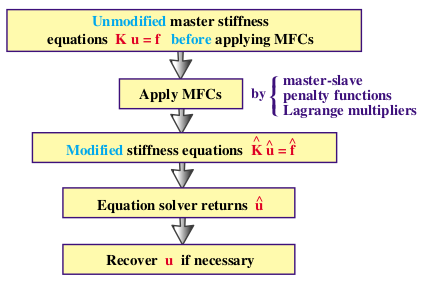
\includegraphics[width=0.70\textwidth]{img/mfc_schematic.png}
    \caption{Schematics of MFC application.}
    \label{fig:MFC-schematic}
\end{figure}


\section{Methods for Imposing MFCs}

Accounting for MFCs is done, at least conceptually, by changing the assembled master
stiffness equations to produce a \textit{modified} system of equations:

\begin{equation}\label{mfc-modification}
    \m{K} \m{u} = \m{f} \overset{MFC}{\implies}
    \hat{\m{K}} \hat{\m{u}} = \hat{\m{f}}
\end{equation}

The modification process \eqref{mfc-modification} is also called  \textit{constraint}
\textit{application} or \textit{constraint imposition}. The modified system
is that submitted to the equation solver, which returns $ \hat{\m{u}} $.

Three methods for applying \textbf{MFCs} are written below:

\begin{enumerate}
    \item \textit{Master-Slave Elimination}

        The DOFs involved in each MFC are separated into master and slave freedoms.
        The slave freedoms are then explicitely eliminated. The modified equations
        do not contain the slave freedoms.

    \item \textit{Penalty Augmentation}

        Also called the \textit{penalty function method}. Each \textbf{MFC}
        is viewed as the presence of a fictious elastic structural element called
        the \textit{penalty element} that enforces it approximately. This element
        is parametrized by a numerical \textit{weight}. The exact constraint is
        recovered if the weight goes to \textbf{infinity}. The MFCs are imposed
        by augmenting the finite element model with the penalty elements.

    \item \textit{Lagrange Multiplier Adjunction}

        For each MFC an additional unknown is adjoined to the master stiffness
        equations. Physically this set of unknowns represent
        \textit{constraint forces} that would enforce the constraints exactly
        should they be applied to the unconstrained system.
\end{enumerate}

The master stiffness equations are assembled ignoring all constraints. Then the MFCs
are imposed by appropriate modification of those equations. There are, however,
two important practical differences:

\begin{enumerate}
    \item The modification process is not unique because there are alternative
        constraint imposition methods. These methods offer tradeofss in generality,
        programming implementation complexity, computational effort, numerical
        accuracy and stability.

    \item In the implementation of some of these methods - notably penalty augmentation
        - constraint imposition and assembly are carried out simultaneously. In that
        case the framework "first assemble, then modify", is not strictly respected
        in the actual implementation.
\end{enumerate}


\subsection{MFC Matrix Forms}

Matrix forms of \textit{linear} \textbf{MFCs} are often convenient for compact
notation. An individual constraint may be written:

\begin{equation}\label{mfc-matrix}
    \begin{bmatrix}
        1 & -2 & 1
    \end{bmatrix}
    \begin{bmatrix}
        u_{x2} \\
        u_{x4} \\
        u_{x6}
    \end{bmatrix}
    = 0.25
\end{equation}

In direct matrix notation:

\begin{equation}\label{mfc-direct}
    \closure{\m{a}}_i \closure{\m{u}}_i = g_i, \quad (no\ sum\ on\ i)
\end{equation}

in which index $ i\ (i = 1, 2,\dots) $ identifies constraint, $ \closure{\m{a}}_i $
is a row vector, $ \closure{\m{u}}_i $ collects the set of \textbf{DOFs}
that participate in the constraint, and $ g_i $ is the \textbf{RHS} scalar.
The bars over $ \m{a} $ and $ \m{u} $ distinguishes
\eqref{mfc-direct} from the expanded form below.

\begin{figure}[ht]
    \centering
    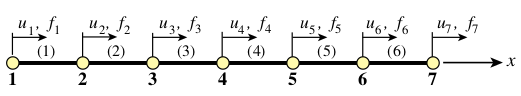
\includegraphics[width=0.70\textwidth]{img/1D_mfc_bar.png}
    \caption{1D problem discretized with six bar finite elements.}
    \label{fig:1D-MFC-bar-png}
\end{figure}

For method description and general proof it is often convenient to \textit{expand}
matrix forms so that they embody \textit{all} DOFs. For example, if
\eqref{mfc-matrix} is a part of a two-dimensional FE model with 12 DOFs:

$ u_{x1}, u_{y1}, \dots, u_{y6} $, the LHS row vector may be expanded with
9 zeros as follows:

\begin{equation}
    \begin{bmatrix}
        0 & 0 & 1 & 0 & 0 & 0 & -2 & 0 & 0 & 0 & 1 & 0
    \end{bmatrix}
    \begin{bmatrix}
        u_{x1} \\
        u_{y1} \\
        u_{x2} \\
        \vdots \\
        u_{y6}
    \end{bmatrix}
    = 0.25
\end{equation}

In which case the matrix notation:

\begin{equation}\label{mfc-expanded}
    \m{a}_i \m{u}_i = g_i
\end{equation}

is used. Finally, all \textbf{MFCs} expressed as \eqref{mfc-expanded} may be collected
into a single matrix relation:

\begin{equation}\label{mfc-expanded-matrix}
    \m{A} \m{u} = \m{g}
\end{equation}

in which the rectangular matrix $ \m{A} $ is formed by stacking the
$ \m{a}_i $'s as rows and column vector $ \m{g} $ is formed by stacking
the $ g_i $s as entries. If there are 12 DOFs in $ \m{u} $ and \textbf{5 MFCs},
then $ \m{A} $ will be $ 5 \times 12 $.


\subsection{The Example Structure}

The one-dimensional FE discretization shown in Figure \ref{fig:1D-MFC-bar-png}
will be used to illustrate the three \textbf{MFC} application methods. The
strucuture consists of six bar elements connected by seven nodes that can only
displace in the \textit{x} direction.

Before imposing various \textbf{multifreedom} constraints discussed below, the master
stiffness equations for this problem are assumed to be:

\begin{equation}\label{master-stiffness-6-bar}
    \begin{bmatrix}
        K_{11} & K_{12} & 0 & 0 & 0 & 0 & 0 \\
        K_{12} & K_{22} & K_{23} & 0 & 0 & 0 & 0 \\
        0 & K_{23} & K_{33} & K_{34} & 0 & 0 & 0 \\
        0 & 0 & K_{34} & K_{44} & K_{45} & 0 & 0 \\
        0 & 0 & 0 & K_{45} & K_{55} & K_{56} & 0 \\
        0 & 0 & 0 & 0 & K_{56} & K_{66} & K_{67} \\
        0 & 0 & 0 & 0 & 0 & K_{67} & K_{77}
    \end{bmatrix}
    \begin{bmatrix}
        u_1 \\
        u_2 \\
        u_3 \\
        u_4 \\
        u_5 \\
        u_6 \\
        u_7
    \end{bmatrix}
    = \begin{bmatrix}
        f_1 \\
        f_2 \\
        f_3 \\
        f_4 \\
        f_5 \\
        f_6 \\
        f_7
    \end{bmatrix}
\end{equation}

or

\begin{equation}\label{mfc-ms-master-equation}
    \m{K} \m{u} = \m{f}
\end{equation}

The nonzero stifness coefficients $ K_{ij} $ in \eqref{master-stiffness-6-bar}
depend on the bar rigidity properties. For example, if
$ E^e A^e / L^e = 100 $ for each element $ e = 1, \dots , 6 $, then
$ K_{11} = K_{77} = 100 $, $ K_{22} = \dots = K_{66} = 200 $,
$ K_{12} = K_{23} = \dots = K_{67} = -100 $. However, for the purposes of the
following treatment the coefficient may be kept arbitrary. The component index
$ x $ in the nodal displacements $ u $ and nodal forces $ f $ has been omitted
for brevity.

Now let us specify a \textbf{MFC} that states that nodes \textbf{2} and \textbf{6}
must move by the same amount:

\begin{equation}\label{mfc-2-6}
    u_2 = u_6
\end{equation}

Passing all node displacements to the RHS gives the canonical form:

\begin{equation}\label{mcf-canonical-2-6}
    u_2 - u_6 = 0
\end{equation}

Constraint conditions of this type are sometimes called \textbf{rigid links}
because they can be mechanically interpreted as forcing node points 2 and 6
to move together as if they were tied tohether by a rigid member.

We now study the imposition of constraint \eqref{mcf-canonical-2-6} on the master equations
\eqref{master-stiffness-6-bar} by the methods mentioned above. First the master-slabe
method is treated

\section{The Master-Slave Method}

To apply this method by \textit{hand}, the MFCs are taken one at a time. For each
constraint a \textbf{slave} DOF is chosen. The freedoms remaining in that constraint
are labeled \textbf{master}. A new set of DOFs $ \m{\hat{u}} $ is established
by removing all slave freedoms from $ \m{u} $. This new vector contains
master freedoms as well as those that do not appear in the MFCs. A matrix transformation
equation that relates $ \m{u} $ to $ \m{\hat{u}} $ is generated. This
equation is used ot apply a congruent transformation to the master stiffness equations.
This procedure yields a set of modified stiffness equations that are expressed in terms
of the new freedom set $ \m{\hat{u}} $. Because the modified system does not contain
the slave freedoms, these have been effectively eliminated.

\subsection{A One-Constraint Example}

The mechanics if the process is best seen by going through an example. To impose
\eqref{mcf-canonical-2-6} pick $ u_6 $ as slave and $ u_2 $ as master. Relate the
original unknowns $ u_1, \dots, u_7 $ to the new set in which $ u_6 $ is missing:

\begin{equation}\label{mfc-ms-transformation}
    \begin{bmatrix}
        u_1 \\
        u_2 \\
        u_3 \\
        u_4 \\
        u_5 \\
        u_6 \\
        u_7
    \end{bmatrix}
    = \begin{bmatrix}
        1 & 0 & 0 & 0 & 0 & 0 \\
        0 & 1 & 0 & 0 & 0 & 0 \\
        0 & 0 & 1 & 0 & 0 & 0 \\
        0 & 0 & 0 & 1 & 0 & 0 \\
        0 & 1 & 0 & 0 & 0 & 0 \\
        0 & 0 & 0 & 0 & 0 & 1
    \end{bmatrix}
    \begin{bmatrix}
        u_1 \\
        u_2 \\
        u_3 \\
        u_4 \\
        u_5 \\
        u_7
    \end{bmatrix}
\end{equation}

This is the required transformation relation. In compact form:

\begin{equation}
    \m{u} = \m{T} \m{\hat{u}}
\end{equation}


Replacing \eqref{mfc-ms-transformation} into \eqref{mfc-ms-master-equation} and
premultiplying by $ \m{T}^T $ yields the modified system:

\begin{equation}\label{mfc-ms-modified-system}
    \m{\hat{K}} \m{\hat{u}} = \m{\hat{f}}, \quad
    in\ which \quad \m{\hat{K}} = \m{T}^T \m{K} \m{T}, \quad
    \m{\hat{f}} = \m{T}^T \m{f}.
\end{equation}

\begin{bbox}
    The form of modified system \eqref{mfc-ms-modified-system} can be remembered
    by a simple mnemonic rule: premultiply both sides of $
    \m{T} \m{\hat{u}} = \m{u} $
    by $ \m{T}^T \m{K} $ and replace $ \m{K} \m{u} $ by
    $ \m{f} $ on the right hand side.
\end{bbox}

Carrying out the indicated matrix multiplication yields:

\begin{equation}\label{mfc-ms-modified-master}
    \begin{bmatrix}
        K_{11} & K_{12} & 0 & 0 & 0 & 0 \\
        K_{12} & K_{22} + K_{66} & K_{23} & 0 & K_{56} & K_{67} \\
        0 & K_{23} & K_{33} & K_{34} & 0 & 0 \\
        0 & 0 & K_{34} & K_{44} & K_{45} & 0 \\
        0 & K_{56} & 0 & K_{45} & K_{55} & 0 \\
        0 & K_{67} & 0 & 0 & 0 & K_{77}
    \end{bmatrix}
    \begin{bmatrix}
        u_1 \\
        u_2 \\
        u_3 \\
        u_4 \\
        u_5 \\
        u_7
    \end{bmatrix}
    = \begin{bmatrix}
        f_1 \\
        f_2 + f_6 \\
        f_3 \\
        f_4 \\
        f_5 \\
        f_7
    \end{bmatrix}
\end{equation}

Equation \eqref{mfc-ms-modified-master} is a new linear system containing 6 equations
in the remaining 6 unknowns $ u_1, u_2, u_3, u_4, u_5\ and\ u_7 $. Upon
solving it, $ u_6 $ is recovered from the constraint \eqref{mfc-2-6}.

\begin{bbox}
    For a simple freedom constraint such as $ u_4 = 0 $ the only possible choice of slave
    is of course $ u_4 $ and there is no master. The congruent transformation is then
    nothing more than the elimination of $ u_4 $ by striking out rows and columns from
    the master stiffness equations.
\end{bbox}


\subsection{Multiple Homogeneous MFCs}

The matrix equation \eqref{mfc-ms-modified-system} in fact holds for the general
case of multiple homogeneous linear constraints. Direct establishment of the transformation
equation, however, is more complicated if slave freedoms in one constraint appear as masters
in another. To illustrate this point, suppose that for the example system we have three
homogeneous MFCs:

\begin{eqarray}\label{mfc-ms-3-constraints}
    u_2 - u_6 &= 0 \\
    u_1 + 4 u_4 &= 0 \\
    2 u_3 + u_4 + u_5 &= 0
\end{eqarray}

Picking as slave freedoms $ u_6 $, $ u_4 $ and $ u_3 $ from the first, second and third
constraint, respectively, we can solve for them as:

\begin{eqarray}
    u_6 &= u_2 \\
    u_4 &= -\frac{1}{4} u_1 \\
    u_3 &= -\frac{1}{2} \left( u_4 + u_5 \right) = \frac{1}{8} u_1 - \frac{1}{2} u_5
\end{eqarray}

Observe that solving for $ u_3 $ from the third constraint brings $ u_4 $ to the RHS.
But because $ u_4 $ is also slave freedom (it was chosen as such for the second constraint)
it is replaced in favor of $ u_1 $ using $ u_4 = -\frac{1}{4} u_1 $. The matrix form
transformation is:

\begin{equation}\label{mfc-ms-multiple-freedoms}
    \begin{bmatrix}
        u_1 \\
        u_2 \\
        u_3 \\
        u_4 \\
        u_5 \\
        u_6 \\
        u_7
    \end{bmatrix}
    = \begin{bmatrix}
        1 & 0 & 0 & 0 \\
        0 & 1 & 0 & 0 \\
        \frac{1}{8} & 0 & -\frac{1}{2} & 0 \\
        -\frac{1}{4} & 0 & 0 & 0 \\
        0 & 0 & 1 & 0 \\
        0 & 1 & 0 & 0 \\
        0 & 0 & 0 & 1
    \end{bmatrix}
    \begin{bmatrix}
        u_1 \\
        u_2 \\
        u_5 \\
        u_7
    \end{bmatrix}
\end{equation}

The modified master system is now formed through the congruent
transformation \eqref{mfc-ms-modified-system}.
Note that the slave freedoms selected from each
constraint must be distinct. For example the choice $ u_6 $, $ u_4 $ and $ u_4 $
would be inadmissible as long the constraints are independent. This rule is easy
to enforce when slave freedoms are chosen by hand, but can lead to implementation
and numerical difficulties when it is programmed as an automated procedure, as
further discussed later.

\begin{bbox}
    The 3 MFCs \eqref{mfc-ms-3-constraints} with $ u_6 $, $ u_4 $ and $ u_2 $ chosen
    as slaves and $ u_1 $, $ u_2 $ and $ u_5 $ chosen as masters, may be presented
    in the partitioned matrix form:

    \begin{equation}
        \begin{bmatrix}
            0 & 0 & 1 \\
            0 & 4 & 0 \\
            2 & 1 & 0
        \end{bmatrix}
        \begin{bmatrix}
            u_3 \\
            u_4 \\
            u_6
        \end{bmatrix}
        = \begin{bmatrix}
            0 & 1 & 0 \\
            -1 & 0 & 0 \\
            0 & 0 & -1
        \end{bmatrix}
        \begin{bmatrix}
            u_1 \\
            u_2 \\
            u_5
        \end{bmatrix}
    \end{equation}

     This may be compactly written as:

     \begin{equation}
         \m{A}_s \m{u}_s + \m{A}_m \m{u}_m = \m{0}
     \end{equation}

     Solving for the slave freedoms gives

     \begin{equation}
         \m{u}_s = -\m{A}_s^{-1} \m{A}_m \m{u}_m
     \end{equation}

     Expanding with zeros to fill out $ \m{u} $ and $ \m{\hat{u}} $
     produces \eqref{mfc-ms-multiple-freedoms}. Note that non-singularity of
     $ \m{A}_s $ is essential for this method to work.
\end{bbox}


\subsection{Nonhomoheneous MFCs}

Extension to nonhomogeneous constraints is immediate. In this case the transformation
equation becomes nonhomogeneous. For example suppose that \eqref{mcf-canonical-2-6}
has non-zero prescribed value:

\begin{equation}\label{mcf-canonical-2-6-nonhomogeneous}
    u_2 - u_6 = 0.2
\end{equation}

Nonzero RHS values such as $ 0.2 $ in \eqref{mcf-canonical-2-6-nonhomogeneous}
may often be interpreted physically as "gaps" (thus the use of the symbol
$ \m{g} $ in the matrix form). Chose $ u_6 $ again as slave: $ u_6 = u_2 - 0.2 $
and build the transformation:

\begin{equation}
    \begin{bmatrix}
        u_1 \\
        u_2 \\
        u_3 \\
        u_4 \\
        u_5 \\
        u_6 \\
        u_7
    \end{bmatrix}
    = \begin{bmatrix}
        1 & 0 & 0 & 0 & 0 & 0 \\
        0 & 1 & 0 & 0 & 0 & 0 \\
        0 & 0 & 1 & 0 & 0 & 0 \\
        0 & 0 & 0 & 1 & 0 & 0 \\
        0 & 0 & 0 & 0 & 1 & 0 \\
        0 & 1 & 0 & 0 & 0 & 0 \\
        0 & 0 & 0 & 0 & 0 & 1
    \end{bmatrix}
    \begin{bmatrix}
        u_1 \\
        u_2 \\
        u_3 \\
        u_4 \\
        u_5 \\
        u_7
    \end{bmatrix} +
    \begin{bmatrix}
        0 \\
        0 \\
        0 \\
        0 \\
        0 \\
        -0.2 \\
        0
    \end{bmatrix}
\end{equation}

In the compact matrix form:

\begin{equation}\label{mfc-ms-gap}
    \m{u} = \m{T} \m{\hat{u}} + \m{g}
\end{equation}

Here the constraint gap vector $ \m{g} $ is nonzero and $ \m{T} $ is the same
as before. To get the modified system applying the shortcut rule, premultiply
both sides of \eqref{mfc-ms-gap} by $ \m{T}^T \m{K} $, replace
$ \m{K} \m{u} $ by $ \m{f} $ and pass the data to the RHS:

\begin{equation}\label{mfc-ms-modified-system-gap}
    \m{\hat{K}} \m{\hat{u}} = \m{\hat{f}}, \quad
    in\ which \quad \m{\hat{K}} = \m{T}^T \m{K} \m{T}, \quad
    \m{\hat{f}} = \m{T}^T \left( \m{f} -\m{K} \m{g} \right).
\end{equation}

Upon solving \eqref{mfc-ms-modified-system-gap} for $ \m{\hat{u}} $, the
complete displacement vector is recovered from \eqref{mfc-ms-gap}. For the MFC
\eqref{mcf-canonical-2-6-nonhomogeneous} this technique gives the system:

\begin{equation}
    \begin{bmatrix}
        K_{11} & K_{12} & 0 & 0 & 0 & 0 \\
        K_{12} & K_{22} + K_{66} & K_{23} & 0 & K_{56} & K_{67} \\
        0 & K_{23} & K_{33} & K_{34} & 0 & 0 \\
        0 & 0 & K_{34} & K_{44} & K_{45} & 0 \\
        0 & K_{56} & 0 & K_{45} & K_{55} & 0 \\
        0 & K_{67} & 0 & 0 & 0 & K_{77}
    \end{bmatrix}
    \begin{bmatrix}
        u_1 \\
        u_2 \\
        u_3 \\
        u_4 \\
        u_5 \\
        u_7
    \end{bmatrix}
    = \begin{bmatrix}
        f_1 \\
        f_2 + f_6 - 0.2 K_{66} \\
        f_3 \\
        f_4 \\
        f_5 - 0.2 K_{56} \\
        f_7 - 0.2 K_{67}
    \end{bmatrix}
\end{equation}


\subsection{The General Case}

For implementation in general-purpose programs the \textbf{master-slave method}
can be described as follows. The \textbf{DOFs} in $ \m{u} $ are classified
into three types: \textbf{independent} or unconstrained, \textbf{masters} and
\textbf{slaves}. The unconstrained DOFs are those that do not appear in any MFC.
Label these sets as $ \m{u}_u $, $ \m{u}_m $ and $ \m{u}_s $,
respectively, and partition the stiffness equations accordingly:

\begin{equation}\label{mfc-ms-partitioned}
    \begin{bmatrix}
        \m{K}_{uu} & \m{K}_{um} & \m{K}_{us} \\
        \m{K}_{um}^T & \m{K}_{mm} & \m{K}_{ms} \\
        \m{K}_{us}^T & \m{K}_{ms}^T & \m{K}_{ss}
    \end{bmatrix}
    \begin{bmatrix}
        \m{u}_u \\
        \m{u}_m \\
        \m{u}_s
    \end{bmatrix}
    = \begin{bmatrix}
        \m{f}_u \\
        \m{f}_m \\
        \m{f}_s \\
    \end{bmatrix}
\end{equation}

The MFCs may be written in matrix form as:

\begin{equation}
    \m{A}_m \m{u}_m + \m{A}_s \m{u}_s = \m{g}_A
\end{equation}

where $ \m{A}_s $ is assumed square and nonsingular. If so we can solve for
the slave freedoms:

\begin{equation}
    \m{u}_s = \m{A}_s^{-1} \m{A}_m \m{u}_m
    + \m{A}_s^{-1} \m{g}_A
    \eqd \m{T} \m{u}_m + \m{g}
\end{equation}

where $ \eqd $ means \textit{equal by definition}. Inserting into the partitioned
sitffness equation \eqref{mfc-ms-partitioned} and symmetrizing yields:

\begin{equation}
    \begin{bmatrix}
        \m{K}_{uu} & \m{\hat{K}}_{um} \\
        \m{\hat{K}}_{um}^T &
        \m{\hat{K}}_{mm}
    \end{bmatrix}
    \begin{bmatrix}
        \m{u}_u \\
        \m{u}_m
    \end{bmatrix}
    = \begin{bmatrix}
        \m{f}_u - \m{K}_{us} \m{g} \\
        \m{f}_m - \m{K}_{ms} \m{g}
    \end{bmatrix}
\end{equation}

where $ \m{\hat{K}}_{um} = \m{K}_{um} + \m{K}_{us} \m{T} $ \\
and $ \m{\hat{K}}_{mm} = \m{K}_{mm} + \m{T}^T \m{K}_{ms}^T
+ \m{K}_{ms} \m{T} + \m{T}^T \m{K}_{ss} \m{T} $.

It is seen that the misleading simplicity of the handworked example is gone.


\subsection{Retaining the Original Freedoms}

A potential disadvantage of the master-slave methid in computer work is that it
requires a rearrangement of the original stiffness equations because
$ \m{\hat{u}} $ is a subset of $ \m{u} $. The disadvantage can be
annoying when sparse matrxi storage schemes are used for the stiffness matrix,
and becomes intolerable if secondary storage is used for that purpose.

With a bit of trickery it is possible to maintain the original freedom ordering.
Let us display it for the example problem under \eqref{mcf-canonical-2-6}.
Instead of \eqref{mfc-ms-transformation}, use the \textit{square} transformation:

\begin{equation}
    \begin{bmatrix}
        u_1 \\
        u_2 \\
        u_3 \\
        u_4 \\
        u_5 \\
        u_6 \\
        u_7
    \end{bmatrix}
    = \begin{bmatrix}
        1 & 0 & 0 & 0 & 0 & 0 & 0 \\
        0 & 1 & 0 & 0 & 0 & 0 & 0 \\
        0 & 0 & 1 & 0 & 0 & 0 & 0 \\
        0 & 0 & 0 & 1 & 0 & 0 & 0 \\
        0 & 0 & 0 & 0 & 1 & 0 & 0 \\
        0 & 1 & 0 & 0 & 0 & 0 & 0 \\
        0 & 0 & 0 & 0 & 0 & 0 & 1
    \end{bmatrix}
    \begin{bmatrix}
        u_1 \\
        u_2 \\
        u_3 \\
        u_4 \\
        u_5 \\
        \overline{u}_6 \\
        u_7
    \end{bmatrix}
\end{equation}

in which $ \overline{u}_6 $ is a \textit{placeholder} for the slave freedom $ u_6 $.
The modified equations are:

\begin{equation}
    \begin{bmatrix}
        K_{11} & K_{12} & 0 & 0 & 0 & 0 & 0 & 0 \\
        K_{12} & K_{22} + K_{66} & K_{23} & 0 & 0 & K_{56} & 0 & K_{67} \\
        0 & K_{23} & K_{33} & K_{34} & 0 & 0 & 0 & 0 \\
        0 & 0 & K_{34} & K_{44} & K_{45} & 0 & 0 & 0 \\
        0 & K_{56} & 0 & K_{45} & K_{55} & 0 & 0 & 0 \\
        0 & K_{67} & 0 & 0 & 0 & 0 & 0 & K_{77}
    \end{bmatrix}
    \begin{bmatrix}
        u_1 \\
        u_2 \\
        u_3 \\
        u_4 \\
        u_5 \\
        \overline{u}_6 \\
        u_7
    \end{bmatrix}
    = \begin{bmatrix}
        f_1 \\
        f_2 + f_6 \\
        f_3 \\
        f_4 \\
        f_5 \\
        0 \\
        f_7
    \end{bmatrix}
\end{equation}

which are submitted to the equation solver. If the solver is not trained to skip
zero rows and columns, a one should be placed in the diagonal entry for the
$ \overline{u}_6 $ equation. The solver will return $ \overline{u}_6 = 0 $,
and this placeholder value is replaced by $ u_2 $.


\subsection{Model Reduction by Kinematic Constraints}

The congruent transformation equations \eqref{mfc-ms-modified-system}
and \eqref{mfc-ms-modified-system-gap} have additional applications beyond the
master-slave method. An important one is \textit{model reduction by kinematic constraints}.
Trough this procedure the number of \textbf{DOFs} of a static or dynamic FEM model
is reduced by a significant number, typycally to $ 1 \% - 10 \% $ of the original number.
This is done by taking a lot of slaves and a few masters. Only the masters are left
after the transformation. The reduced model is commonly used in subsequent calculations
as a component of a larger system, particularly during design or in parameter
identification.


\textbf{Example:}

\begin{figure}[ht]
    \centering
    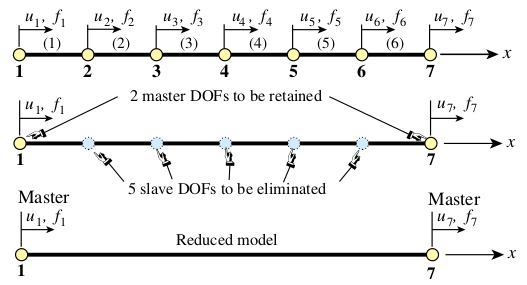
\includegraphics[width=0.90\textwidth]{img/mfc_model_reduction_end.png}
    \caption{Model reduction of the example structure to the end freedoms}
    \label{fig:mfc-model-reduction-end-png}
\end{figure}

Consider the bar assembly of Figure \ref{fig:mfc-model-reduction-end-png}.
Assume that the only masters are the end motions $ u_1 $ and $ u_7 $, as
illustrated in Figure \ref{fig:mfc-model-reduction-end-png}, and interpolate
all freedoms linearly:

\begin{equation}
    \begin{bmatrix}
        u_1 \\
        u_2 \\
        u_3 \\
        u_4 \\
        u_5 \\
        u_6 \\
        u_7
    \end{bmatrix}
    = \begin{bmatrix}
        1 & 0 \\
        \frac{5}{6} & \frac{1}{6} \\
        \frac{4}{6} & \frac{2}{6} \\
        \frac{3}{6} & \frac{3}{6} \\
        \frac{2}{6} & \frac{4}{6} \\
        \frac{1}{6} & \frac{5}{6} \\
        0 & 1 \\
    \end{bmatrix}
    \begin{bmatrix}
        u_1 \\
        u_7
    \end{bmatrix}, \quad or \quad
    \m{u} = \m{T} \m{\hat{u}}
\end{equation}

The reduced-order-model (\textbf{ROM}) equations are:

\begin{equation}
    \m{\hat{k}} \m{\hat{u}}
    = \m{T}^T \m{K} \m{T} \m{\hat{u}}
    = \m{T}^T \m{f}
    = \m{\hat{f}}
\end{equation}

or in detail

\begin{equation}
    \begin{bmatrix}
        \hat{K}_{11} & \hat{K}_{17} \\
        \hat{K}_{17}^T & \hat{K}_{77}
    \end{bmatrix}
    \begin{bmatrix}
        u_1 \\
        u_7
    \end{bmatrix}
    = \begin{bmatrix}
        \hat{f}_1 \\
        \hat{f}_7
    \end{bmatrix}
\end{equation}

in which:

\begin{eqarray}
    \hat{K}_{11} &= \frac{1}{36}
    \left( 36 K_{11} + 60 K_{12} + 25 K_{22} + 40 K_{23} + 16 K_{33} + 24 K_{34} \right. \\
                 &+  \left. 9 K_{44} + 12 K_{45} + 4 K_{55} + 4 K_{56} + K_{66} \right) \\
    \hat{K}_{17} &= \frac{1}{36}
    \left( 6 K_{12} + 5 K_{22} + 14 K_{23} + 8 K_{33} + 18 K_{34} + 9 K_{44} \right. \\
                 &+ \left. 18 K_{45} + 8 K_{55} + 14 K_{56} + 5 K_{66} + 6 K_{67} \right) \\
    \hat{K}_{77} &= \frac{1}{36}
    \left( K_{22} + 4 K_{23} + 4 K_{33} + 12 K_{34} + 9 K_{44} + 24 K_{45} \right. \\
                 &+ \left. 16 K_{55} + 40 K_{56} + 25 K_{66} + 60 K_{67} + 36 K_{77} \right) \\
    \hat{f}_1 & = \frac{1}{6}
    \left(
        6 f_1 + 5 f_2 + 4 f_3 + 3 f_4 + 2 f_5 + f_6
    \right) \\
    \hat{f}_7 & = \frac{1}{6}
    \left(
        f_2 + 2 f_3 + 3 f_4 + 4 f_5 + 5 f_6 + 6 f_7
    \right) \\
\end{eqarray}

This reduces the order of the FEM model from 7 to 2. The \textbf{key feature} is that
the masters are picked \textbf{a priori}, as the freedoms to be retained in the
model for further use.

\begin{bbox}
    Model reduction can be also done by the \textbf{static condensation} (Guyan)
    method. As its name indicates, condensation is restricted to static analysis.
    On the other hand, for such problems it is exact whereas model reduction by
    kinematic constraints generally introduces approximations.
\end{bbox}


\subsection{Assesment of the Master-Slave Method}

The \textbf{Master-Slave Method} enjoys the advantage of being \textbf{exact}
(except for inevitable solution errors from finite number precision) and of
reducing the nuber of unknowns. The concept is also easy to explain and learn.
The main implementation drawback is the complexity of the general case.
The complexity is due to three factors:

\begin{enumerate}
    \item The equations may have to be rearranged because of the disappearance
        of the slave freedoms. This drawback can be alleviated, however,
        by the \textbf{placeholder} trick.

    \item An auxiliary linear system has to be assembled and solved to produce
        the transformation matrix $ \m{T} $ and vector $ \m{g} $.

    \item The transformation process may generate many additional matrix terms.
        If a sparse matrix storage scheme is used for $ \m{K} $, the logic
        for allocating memory and storing these entries can be difficult
        and expensive.
\end{enumerate}

The level of complexity depends on the generality allowed as well as on programming
decisions. If $ \m{K} $  is stored as full matrix and slave freedom coupling in
the MFCs is disallowed the logic is simple (this is the case in model reduction,
since each slave freedom appears in one and only one MFC). On the other hand,
if arbitrary couplings are permitted and $ \m{K} $ is placed in secondary
(disk) storage according to some sparse scheme, the complexity can become
overwhelming.

Another, more subtle, drawback of this method is that it requires decisions as to
which DOFs are to be treated as slaves. This can lead to implementation and numerical
stability problems. Although for disjointed constraints the process can be programmed
in reliable form, in more general cases of coupled constraint equations it can
lead to incorrect decisions. For example, suppose that in the example problem
you have the following two MFCs:

\begin{eqarray}
    \frac{1}{6} u_2 + \frac{1}{2} u_4 &= u_6 \\
    u_3 + 6 u_6 &= u_7
\end{eqarray}

For numerical stability reasons it is usually better to pick as slaves the freedoms
with largest coefficients. If this is done, the program would select $ u_6 $ as
slave freedoms from both constraints. This leads to a contradiction because
having two constraints we must eliminate two slave DOFs, not just one. The resulting
modified system would in fact be inconsistent. Although this defect can be easily fixed
by the program logic in this case, one can imagine the complexity burden if faced
with hundreds of thousands of MFCs.

Serious numerical problems can arise if the MFCs are not independent. For example:

\begin{eqarray}
    \frac{1}{6} u_2 &= u_6 \\
    \frac{1}{3} u_3 + 6 u_6 &= u_7 \\
    u_2 + u_3 - u_7 &= 0
\end{eqarray}

The last constraint is an exact linear combination of the first two. If the program
blindly choses $ u_2 $, $ u_3 $ and $ u_7 $ as slaves, the modified system is
incorrect because we eliminate three equations when in fact there are only two
independent constraints. Exact linear dependence, as before, can be recognised by
a rank analysis of the $ \m{A}_s $ matrix defined. In the floating-point
arithmetic, however, such detection may fail because that kind of computation is
inexact bt nature (The safest technique to identify dependencies is to do
a singular value decomposition (SVD) of $ \m{A}_s $. This can be, however,
prohibitively expensive if one is dealing with hundreds of thousands of constraints.).

The complexithy of slave selection is in fact equivalent to that of automatically
selecting kinematic redundancies in the Force Method of structural analysis.
\textbf{It has led implementators of programs that use this method to require masters}
\textbf{and slaves to be prescribed in the input data, thus transfering the burden}
\textbf{to users}.

The method is not generally extensible to nonlinear constraints without case
by case programming.

In conclusion, the master-slave method is useful when a few simple linear constraints
are imposed by hand. As a general purpose technique for FEM it suffers from
complexity and lack of robustness. It is worth learning, however, because of the
great importance of congruent transformations in
\textit{model reduction} for static and dynamic problems.

\subsubsection{Bibliograpy}

Felippa - IFEM (Chapter 8)

Zienkiewicz and Taylor - The Finite Element Method \textit{4th ed.} 1988


\section{The Penalty Method}

\begin{figure}[ht]
    \centering
    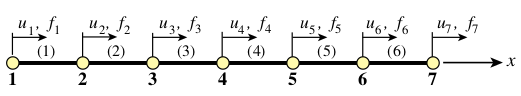
\includegraphics[width=0.70\textwidth]{img/1D_mfc_bar.png}
    \caption{1D problem discretized with six bar finite elements.}
    \label{fig:1D-MFC-bar-png-2}
\end{figure}

The penalty method will be first presented using a physical interpretation,
leaving the mathematical formulation to a subsequent section. Constider again
the bar example structure. To impose $ u_2 = u_6 $ imagine that nodes 2 and 6
are connected with a "fat" bar of axial stiffness $ w $, labeled with element
number 7, as shown in Figure \ref{fig:1D-MFC-bar-penalty-png}. This bar is called \textbf{penalty element} and
$ w $ is its \textbf{penalty weight}.

\begin{figure}[ht]
    \centering
    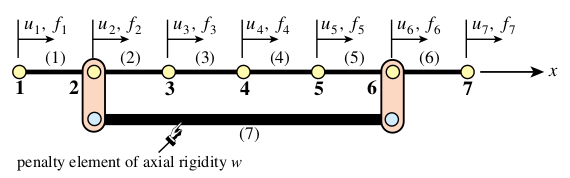
\includegraphics[width=0.70\textwidth]{img/1D_mfc_bar_penalty.png}
    \caption{Adjusnction of a fictious penalty bar of axial stiffness $ w $,
    identified as element 7, to enforce $ u_2 = u_6 $.}
    \label{fig:1D-MFC-bar-penalty-png}
\end{figure}

Such an element, albeit fictious, can be treated exactly like another bar element
insofar as continuing the assembly of the master stiffness equations. The penalty
element stiffness equations $ \m{K}^{(7)} \m{u}^{(7)} = \m{f}^{(7)} $,
are:

\begin{equation}
    w \begin{bmatrix}
        \phantom{-}1 & -1 \\
        -1 & \phantom{-}1
    \end{bmatrix}
    \begin{bmatrix}
        u_2 \\
        u_6
    \end{bmatrix}
    = \begin{bmatrix}
        f_2^{(7)} \\
        f_6^{(7)}
    \end{bmatrix}
\end{equation}

Because there is one freedom per node, the two local element freedoms map into global
freedoms 2 and 6, respectively. Using the assembly rules we obtain the following
modified master stiffness equations: $ \m{\hat{K}} \m{\hat{u}} = \m{\hat{f}} $,
which shown in detail are:

\begin{equation}\label{mfc-penalty-master-stiffnes}
    \begin{bmatrix}
        K_{11} & K_{12} & 0 & 0 & 0 & 0 & 0 \\
        K_{12} & K_{22} + w & K_{23} & 0 & 0 & -w & 0 \\
        0 & K_{23} & K_{33} & K_{34} & 0 & 0 & 0 \\
        0 & 0 & K_{34} & K_{44} & K_{45} & 0 & 0 \\
        0 & 0 & 0 & K_{45} & K_{55} & K_{56} & 0 \\
        0 & -w & 0 & 0 & K_{56} & K_{66} + w & K_{67} \\
        0 & 0 & 0 & 0 & 0 & K_{67} & K_{77}
    \end{bmatrix}
    \begin{bmatrix}
        u_1 \\
        u_2 \\
        u_3 \\
        u_4 \\
        u_5 \\
        u_6 \\
        u_7
    \end{bmatrix}
    = \begin{bmatrix}
        f_1 \\
        f_2 \\
        f_3 \\
        f_4 \\
        f_5 \\
        f_6 \\
        f_7
    \end{bmatrix}
\end{equation}

This system can now be submitted to the equation solver. Note that
$ \m{\hat{u}} \equiv \m{u} $ and only $ \m{K} $ has changed.

\subsection{Choosing the Penalty Weight}

What happens when \eqref{mfc-penalty-master-stiffnes} is solved numerically?
If a \textit{finite} weight $ w $ is chosen the constraint $ u_2 = u_6 $ is
approximately satisfied in the sense that one gets $ u_2 - u_6 = e_g $, where
$ e_g \neq 0 $. The "gap error" $ e_g $ is called the \textit{constraint violation}.
The magnitude $ \left| e_g \right| $ of this violation depends on the wight:
the larger $ w $, the smaller the violation. More precisely, it can be shown
that $ | e_g | $ becomes ptoportional to $ \frac{1}{w} $ as $ w $ gets to be
sufficiently large. For example, raising $ w $ from, say, $ 10^6 $ to $ 10^7 $
can be expected to cut the constraint violation roughly by $ 10 $ if the physical
stiffnesses are smalle compared to $ w $.

Therefore it seems as if the proper strategy should be: try to make $ w $ as large
as possible while respecting the computer overflow limits. However, this is misleading.
As the penalty weight $ w $ tends to $ \infty $ the modified stiffness matrix becomes
more and more \textit{ill-conditioned with respect to inversion}.

To make this point clear, suppose for definiteness that rigidites
$ E^e A^e / L^e $ of the actual bars $ e = 1, \dots, 6 $ are unity, that
$ w >> 1 $, and that the computer solving the stiffness equations has a
floating-point precision of 16 decimal places. Numerical analusts characterize such
precision by sayinf that $ \epsilon_f = \mathcal{O}(10^{-16}) $, where
$ | \epsilon_f | $ is the smallest power of 10 that perceptibly adds to 1 in
floating-point arithmetic (this is usually done not for decimal numbers but
base-2 binary numbers). The modified stiffness matrix of \eqref{mfc-penalty-master-stiffnes}
becomes:

\begin{equation}
    \m{\hat{K}} =
    \begin{bmatrix}
        \phantom{-}1 & -1 & \phantom{-}0 & \phantom{-}0 & \phantom{-}0 & \phantom{-}0 & \phantom{-}0 \\
        -1 & 2+w & -1 & \phantom{-}0 & \phantom{-}0 & -w & \phantom{-}0 \\
        \phantom{-}0 & -1 & \phantom{-}2 & -1 & \phantom{-}0 & \phantom{-}0 & \phantom{-}0 \\
        \phantom{-}0 & \phantom{-}0 & -1 & \phantom{-}2 & -1 & \phantom{-}0 & \phantom{-}0 \\
        \phantom{-}0 & \phantom{-}0 & \phantom{-}0 & -1 & \phantom{-}2 & -1 & \phantom{-}0 \\
        \phantom{-}0 & -w & \phantom{-}0 & \phantom{-}0 & -1 & 2+w & -1 \\
        \phantom{-}0 & \phantom{-}0 & \phantom{-}0 & \phantom{-}0 & \phantom{-}0 & -1 & \phantom{-}1
    \end{bmatrix}
\end{equation}

Clearly as $ w \rightarrow \infty $ rows 2 and 6, as well as columns 2 and 6, tend
to become linearly dependent, in fact the negative of each other. But
\textbf{linear dependency means singularity!} Thus $ \m{\hat{K}} $
approaches singularity as $ w \rightarrow \infty $. In fact, if $ w $ exceeds
$ 1 / \epsilon_f = 10^16 $ the computer will not be able to distinguish
$ \m{\hat{K}} $ from an exactly singular matrix. If $ w << 10^16 $, the
effect will be seen in increasing solution errors affecting the computed
displacements $ \m{\hat{u}} $ returned by the equation solver.
These errors, however, tend to be more random in nature than the constraint
violation error.

\subsection{The Square Root Rule}

Obviously we have two effects at odds with each other. Making $ w $ larger
reduces the constraint violation error but increases the solution error. The
best $ w $ is that which makes both errors roughly equal in absolute value.
This tradeoff value is difficult to find aside of systematicelly running
numerical experiments. In practice \textit{square root rule} is often followed.

This rule can be stated as follows:

Suppose that the largest stiffness coefficient, before adding penalty elements,
is of the order of $ 10^k $ and that the working machine precision is $ p $
digits (such order-of magnitude estimates can be easily found by scanning just
the diagonal of $ \m{K} $). Then choose penalty weights to be of order
$ 10^{k+p/2} $ with the proviso that such a choice would not cause aritmetic
overflow (if overflow occurs, the master stiffness matrix should be scaled
throughout or a better choice of physical units made).

For the above example in which $ k \approx 0 $ and $ p \approx 16 $, the
optimal $ w $ given by this rule would be $ w \approx 10^8 $.
This $ w $ would yield a constraint violation and a solution error of order
$ 10^{-8} $. Note that there is no simple way to do better than this accuracy
aside from using \textbf{extended floating-point precision}. This is not
easy to do when using standard low-level programming languages.

The name "square root@ arises because the recommended $ w $ is in fact
$ 10^k \sqrt{10^p} $. It is seen that picking the weight by this rule requires
knowledge of both stiffness magnitudes and floating-point hardware properties
of the computer used, as well as the precision selected by the program.


\subsection{Penalty Elements for General MFCs}

For the constraint $ u_2 = u_6 $ the physical interpretation of the penalty
element is clear. Points 2 and 6 must move in lockstep along $ x $, which
can be approximately enforced by the heavy bar device. But how about
$ 3 u_3 + u_5 - 4 u_6 = 1 $ or just $ u_2 = -u_6 $?

The treatment of more general constraints is linked to the theory of
\textit{Courant penalty functions} from the \textit{variational calculus}.
Consider the homogenenous constraint:

\begin{equation}
    4 u_3 + u_5 - 4 u_6 = 0
\end{equation}

Rewrite this equation in matrix form:

\begin{equation}
    \begin{bmatrix}
        3 & 1 & -4
    \end{bmatrix}
    \begin{bmatrix}
        u_3 \\
        u_5 \\
        u_6
    \end{bmatrix}
    = 0
\end{equation}

and premultiply both sides by the transpose of the coefficient matrix:

\begin{equation}
    \begin{bmatrix}
        3 \\
        1 \\
        -4
    \end{bmatrix}
    \begin{bmatrix}
        3 & 1 & -4
    \end{bmatrix}
    \begin{bmatrix}
        u_3 \\
        u_5 \\
        u_6
    \end{bmatrix}
    =
    \begin{bmatrix}
        9 & 3 & -12 \\
        3 & 1 & -4 \\
        -12 & -4 & 16
    \end{bmatrix}
    \begin{bmatrix}
        u_3 \\
        u_5 \\
        u_6
    \end{bmatrix}
    = \m{\closure{K}}^e \m{u} = 0
\end{equation}

Here $ \m{\closure{K}}^e $ is the \textit{unscaleed} stiffness matrix of
the penalty element. This is now multiplied by the penalty weight $ w $ and
assembled into the master stiffness matrix following the usual rules. For the
example problem, augmentint the master stiffness matrix with the $ w $-scaled
penalty element yields:

\begin{equation}
    \begin{bmatrix}
        K_{11} & K_{12} & 0 & 0 & 0 & 0 & 0 \\
        K_{12} & K_{22} & K_{23} & 0 & 0 & 0 & 0 \\
        0 & K_{23} & K_{33} + 9 w & K_{34} & 3w & -12w & 0 \\
        0 & 0 & K_{34} & K_{44} & K_{45} & 0 & 0 \\
        0 & 0 & 3w & K_{45} & K_{55} + w & K_{56} - 4w & 0 \\
        0 & 0 & -12w & 0 & K_{56} - 4w & K_{66} + 16w & K_{67} \\
        0 & 0 & 0 & 0 & 0 & K_{67} & K_{77}
    \end{bmatrix}
    \begin{bmatrix}
        u_1 \\
        u_2 \\
        u_3 \\
        u_4 \\
        u_5 \\
        u_6 \\
        u_7
    \end{bmatrix}
    = \begin{bmatrix}
        f_1 \\
        f_2 \\
        f_3 \\
        f_4 \\
        f_5 \\
        f_6 \\
        f_7
    \end{bmatrix}
\end{equation}

If the constraint is nonhomogeneous the force vector is also modified. To illustrate this
effect, consider the MFC: $ 3 u_3 + u_5 - 4 u_6 = 1 $. Rewrite this in matrix form as:

\begin{equation}
    \begin{bmatrix}
        3 & 1 & -4
    \end{bmatrix}
    \begin{bmatrix}
        u_3 \\
        u_5 \\
        u_6
    \end{bmatrix}
    = 1
\end{equation}

Premultiply both sides by the transpose of the coefficient matrix:

\begin{equation}
    \begin{bmatrix}
        9 & 3 & -12 \\
        3 & 1 & -4 \\
        -12 & -4 & 16
    \end{bmatrix}
    \begin{bmatrix}
        u_3 \\
        u_5 \\
        u_6
    \end{bmatrix}
    = \begin{bmatrix}
        3 \\
        1 \\
        -4
    \end{bmatrix}
\end{equation}

Scaling by $ w $ and assembling yields:

\begin{equation}
    \resizebox{0.85\hsize}{!}{%
        $\begin{bmatrix}
            K_{11} & K_{12} & 0 & 0 & 0 & 0 & 0 \\
            K_{12} & K_{22} & K_{23} & 0 & 0 & 0 & 0 \\
            0 & K_{23} & K_{33} + 9 w & K_{34} & 3w & -12w & 0 \\
            0 & 0 & K_{34} & K_{44} & K_{45} & 0 & 0 \\
            0 & 0 & 3w & K_{45} & K_{55} + w & K_{56} - 4w & 0 \\
            0 & 0 & -12w & 0 & K_{56} - 4w & K_{66} + 16w & K_{67} \\
            0 & 0 & 0 & 0 & 0 & K_{67} & K_{77}
        \end{bmatrix}
        \begin{bmatrix}
            u_1 \\
            u_2 \\
            u_3 \\
            u_4 \\
            u_5 \\
            u_6 \\
            u_7
        \end{bmatrix}
        = \begin{bmatrix}
            f_1 \\
            f_2 \\
            f_3 + 3 w \\
            f_4 \\
            f_5 + w \\
            f_6 - 4 w \\
            f_7
        \end{bmatrix}$
    }
\end{equation}


\subsection{The Theory Behind the Penalty Method Coefficient Matrix}

The rule of \textit{Courant penalty functions} comes from the following
mathematical theory. Suppose we have a set of $ m $ linear MFCs. Using
the matrix notation introduced, these will be stated as:

\begin{equation}
    \m{a}_p \m{u} = b_p, \quad p = 1, \dots, m
\end{equation}

where $ \m{u} $ contains all DOFs and each $ \m{a}_p $ is a row vector
with the same length as $ \m{u} $. To incorporate the MFCs into the FEM
model one selects a weight $ w_p > 0 $ for each constraint and constructs the
so-called \textbf{Courant quadratic penalty function} or "penalty energy":

\begin{equation}
    P = \sum_{p=1}^m P_p,\ with\ 
    P_p = \m{u}^T \left(
        \frac{1}{2} \m{a}_p^T \m{a}_p \m{u}
        - w_p \m{a}_p^T b_p
        \right)
        = \frac{1}{2} \m{u}^T \m{K}^{(p)} \m{u}
        - \m{u}^T \m{f}^{(p)}
\end{equation}

where we have called $ \m{K}^{(p)} = w_p \m{a}_p^T \m{a}_p $
and $ \m{f}^{(p)} = w_p \m{a}^T b_p $. $ P $ is added to the potential
energy function
$ \prod = \frac{1}{2} \m{u}^T \m{K} \m{u} - \m{u}^T \m{f} $
to form the \textit{augmented potential energy} $ \prod_a = \prod + P $.
Minimization of $ \prod_a $ with respect to $ \m{u} $ yields:

\begin{equation}\label{mfc-augmented-potential-energy}
    \left( \m{K} \m{u} + \sum_{p=1}^m \m{K}^{(p)} \right) \m{u}
    = \m{f} + \sum_{p=1}^m \m{f}^{(p)}
\end{equation}

Each term of the sum on $ p $, which derives from term $ P_p $ may be viewed as
contributed by a penalty element with globalised stiffness matrix
$ \m{K}^{(p)} = w_p \m{a}_p^T \m{a}_p $ and globalised added
force term $ \m{f}^{(p)} = w_p \m{a}_p^T b_p $.

To use a even more compact form we may write the set of MFCs as
$ \m{A} \m{u} = \m{b} $. Then the penalty augmented system can
be written compactly as:

\begin{equation}
    \left( \m{K} + \m{A}^T \m{W} \m{A} \right) \m{u}
    = \m{f} + \m{W} \m{A}^T \m{b}
\end{equation}

where $ \m{W} $ is a diagonal matrix of penalty weights. This compact form,
however, conceals the configuration of the penalty elements.


\subsection{Assesment of the Penalty Method}

The main advantage of the penalty function method is its straightforward computer
implementation. Looking at the modified systems it is obvious that master equations
need not be rearranged. That is, $ \m{u} $ and $ \m{\hat{u}} $ are the same.
Constraints may be programmed as "penalty elements", and stiffness and force
contributions fo these elements merged through the standard assembler. In fact
using this method there is no need to distinguish between unconstrained and
constrained equations! Once all elements - regular and penalty - are assembled,
the system can be passed to the equation solver. \textbf{Single Freedom Constraints},
are usually processed separately for efficiency.

An important advantage with respect to the master-slave (elimination) method
is its lack of sensitivity with respect to whether constraints are linearly
dependent. To give a simplistic example, suppose that the constraint
$ u_2 = u_6 $ appears twice. Then two penalty elements connecting 2 and 6 will
be inserted, doubling the intended weight but not otherwise causing undue harm.

An advantage with respect to the Lagrange multiplier method is that positive
definiteness is not lost. Such loss can affect the performance of certain numerical
processes (for example solving the master stiffness equations by Cholesky
factorisation or conjugate-gradients). Finally, it is worth noting that the
penalty method is easily extensible to nonlinear constraints.

The main disadvantage, however, is a serious one: the choice of weight values
that balance solution accuracy with the violation of constraint conditions.
For simple cases the square root rule previously described often works, although
its effective use calls for knowledge og the magnitude of stiffness coefficients.
Such knowledge may be difficult to extract from general purpose "black box" program.
For difficult cases selection of appropriate weights may require extensive
numerical experimentation, wasting the user time with numerical games that have
no bearing on the actual objective, which is getting a solution.

The deterioration of the condition number fo the penalty-augmented stiffness
matrix can have serious side effects in some solution procedures such as
eigenvalue extraction or iterative solver.

Finally, even if optimal weights are selected, the combined solution error cannot
be lowered beyond a treshold value.

From this assessment it is evident that penalty augmentation, although superior
to the master-slave method from the standpoint of generality and ease of
implementation, is no panacea.


\section{Lagrange Multiplier Adjuction}

\begin{figure}[ht]
    \centering
    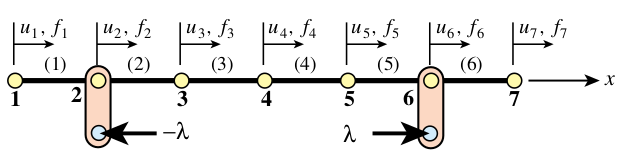
\includegraphics[width=0.70\textwidth]{img/1D_mfc_lagrange_multiplier.png}
    \caption{Physical interpretation of Lagrange multiplier adjuction to enforce
    the MFC $ u_2 = u_6 $}
    \label{fig:1D-MFC-lagrange-multiplier-png}
\end{figure}


\subsection{Physical Interpretation}

As in the case of the penalty function method, the method Lagrange multiplier
can be given a rigorous justification within the framework of variational
calculus. But in the same spirit it will be introduced for the example structure
from a physical standpoint that is particularly illuminating.

Consider again the constraint $ u_2 = u_6 $. Borrowing some ideas from the
penalty method, imagine that nodes 2 and 6 are connected now by
a \textit{rigis} link rather than a flexible one. Thus the constraint is imposed
exactly. But of course the penalty method with an infinite weight would "blow up".

We may remove the link if it is replaced by an appropriate reaction force pair
$ ( -\lambda, +\lambda ) $, as illustrated in Figure
\ref{fig:1D-MFC-lagrange-multiplier-png}. These are called the
\textit{constraint forces}. Incorporating these forces into the original stiffness
equations we get:

\begin{equation}\label{master-stiffness-6-bar-lagrange}
    \begin{bmatrix}
        K_{11} & K_{12} & 0 & 0 & 0 & 0 & 0 \\
        K_{12} & K_{22} & K_{23} & 0 & 0 & 0 & 0 \\
        0 & K_{23} & K_{33} & K_{34} & 0 & 0 & 0 \\
        0 & 0 & K_{34} & K_{44} & K_{45} & 0 & 0 \\
        0 & 0 & 0 & K_{45} & K_{55} & K_{56} & 0 \\
        0 & 0 & 0 & 0 & K_{56} & K_{66} & K_{67} \\
        0 & 0 & 0 & 0 & 0 & K_{67} & K_{77}
    \end{bmatrix}
    \begin{bmatrix}
        u_1 \\
        u_2 \\
        u_3 \\
        u_4 \\
        u_5 \\
        u_6 \\
        u_7
    \end{bmatrix}
    = \begin{bmatrix}
        f_1 \\
        f_2 - \lambda \\
        f_3 \\
        f_4 \\
        f_5 \\
        f_6 + \lambda \\
        f_7
    \end{bmatrix}
\end{equation}

This $ \lambda $ is called \textbf{Lagrange multiplier}. Because $ \lambda $
is an unknown, let us transfer it to the \textbf{LHS} by \textbf{appending} it
to the vector of unknowns:

\begin{equation}
    \begin{bmatrix}
        K_{11} & K_{12} & 0 & 0 & 0 & 0 & 0 & 0 \\
        K_{12} & K_{22} & K_{23} & 0 & 0 & 0 & 0 & 1 \\
        0 & K_{23} & K_{33} & K_{34} & 0 & 0 & 0 & 0 \\
        0 & 0 & K_{34} & K_{44} & K_{45} & 0 & 0 & 0 \\
        0 & 0 & 0 & K_{45} & K_{55} & K_{56} & 0 & 0 \\
        0 & 0 & 0 & 0 & K_{56} & K_{66} & K_{67} & -1 \\
        0 & 0 & 0 & 0 & 0 & K_{67} & K_{77} & 0
    \end{bmatrix}
    \begin{bmatrix}
        u_1 \\
        u_2 \\
        u_3 \\
        u_4 \\
        u_5 \\
        u_6 \\
        u_7 \\
        \lambda
    \end{bmatrix}
    = \begin{bmatrix}
        f_1 \\
        f_2 \\
        f_3 \\
        f_4 \\
        f_5 \\
        f_6 \\
        f_7
    \end{bmatrix}
\end{equation}

But now we have 7 equations for 8 unknowns. To render the system determinate, the
constraint condition $ u_2 - u_6 = 0 $ is appended as eight equation:

\begin{equation}
    \begin{bmatrix}
        K_{11} & K_{12} & 0 & 0 & 0 & 0 & 0 & 0 \\
        K_{12} & K_{22} & K_{23} & 0 & 0 & 0 & 0 & 1 \\
        0 & K_{23} & K_{33} & K_{34} & 0 & 0 & 0 & 0 \\
        0 & 0 & K_{34} & K_{44} & K_{45} & 0 & 0 & 0 \\
        0 & 0 & 0 & K_{45} & K_{55} & K_{56} & 0 & 0 \\
        0 & 0 & 0 & 0 & K_{56} & K_{66} & K_{67} & -1 \\
        0 & 0 & 0 & 0 & 0 & K_{67} & K_{77} & 0 \\
        0 & 1 & 0 & 0 & 0 -1 & 0 & 0
    \end{bmatrix}
    \begin{bmatrix}
        u_1 \\
        u_2 \\
        u_3 \\
        u_4 \\
        u_5 \\
        u_6 \\
        u_7 \\
        \lambda
    \end{bmatrix}
    = \begin{bmatrix}
        f_1 \\
        f_2 \\
        f_3 \\
        f_4 \\
        f_5 \\
        f_6 \\
        f_7 \\
        0
    \end{bmatrix}
\end{equation}

This is called the \textbf{multiplier-augmented} system. Its coefficient matrix,
which is symmetric, is called the \textbf{bordered stiffness matrix}. The
process by which $ \lambda $ is appended to the vector of original unknowns
is called \textbf{adjucation}. Solving this system provides the desired solution
for the DOFs while also characterising the constraint forces through
$ \lambda $.


\subsection{Lagrange Multipliers fro General MFCs}

The general procedure will be stated first as a recipe. Suppose that we want
to solve the example structure subjected to three MFCs:

\begin{equation}
    u_2 - u_6 = 0, \quad 5 u_2 - 8 u_7 = 3, \quad 3 u_3 + u_5 - 4 u_6 = 1
\end{equation}

Adjoin these MFCs as the eighth, nineth, and tenth equations:

\begin{equation}
    \begin{bmatrix}
        K_{11} & K_{12} & 0 & 0 & 0 & 0 & 0 \\
        K_{12} & K_{22} & K_{23} & 0 & 0 & 0 & 0 \\
        0 & K_{23} & K_{33} & K_{34} & 0 & 0 & 0 \\
        0 & 0 & K_{34} & K_{44} & K_{45} & 0 & 0 \\
        0 & 0 & 0 & K_{45} & K_{55} & K_{56} & 0 \\
        0 & 0 & 0 & 0 & K_{56} & K_{66} & K_{67} \\
        0 & 0 & 0 & 0 & 0 & K_{67} & K_{77} \\
        0 & 1 & 0 & 0 & 0 & -1 & 0 \\
        0 & 5 & 0 & 0 & 0 & 0 & -8 \\
        0 & 0 & 3 & 0 & 1 & -4 & 0
    \end{bmatrix}
    \begin{bmatrix}
        u_1 \\
        u_2 \\
        u_3 \\
        u_4 \\
        u_5 \\
        u_6 \\
        u_7
    \end{bmatrix}
    = \begin{bmatrix}
        f_1 \\
        f_2 \\
        f_3 \\
        f_4 \\
        f_5 \\
        f_6 \\
        f_7 \\
        0 \\
        3 \\
        1
    \end{bmatrix}
\end{equation}

Three Lagrange multipliers: $ \lambda_1, \lambda_2 $ and $ \lambda_3 $ are
required to care of three MFCs. Adjoin those unknowns to the nodal displacement
vector. Symmetrize the coefficient matrix by appending 3 columns that are the
transpose of the 3 last rows and filling the bottom righ-hand corner with
a $ 3 \times 3 $ zero matrix:

\begin{equation}
    \begin{bmatrix}
        K_{11} & K_{12} & 0 & 0 & 0 & 0 & 0 & 0 & 0 & 0 \\
        K_{12} & K_{22} & K_{23} & 0 & 0 & 0 & 0 & 1 & 5 & 0 \\
        0 & K_{23} & K_{33} & K_{34} & 0 & 0 & 0 & 0 & 0 & 3 \\
        0 & 0 & K_{34} & K_{44} & K_{45} & 0 & 0 & 0 & 0 & 0 \\
        0 & 0 & 0 & K_{45} & K_{55} & K_{56} & 0 & 0 & 0 & 1 \\
        0 & 0 & 0 & 0 & K_{56} & K_{66} & K_{67} & -1 & 0 & -4 \\
        0 & 0 & 0 & 0 & 0 & K_{67} & K_{77} & 0 & -8 & 0 \\
        0 & 1 & 0 & 0 & 0 & -1 & 0 & 0 & 0 & 0 \\
        0 & 5 & 0 & 0 & 0 & 0 & -8 & 0 & 0 & 0 \\
        0 & 0 & 3 & 0 & 1 & -4 & 0 & 0 & 0 & 0
    \end{bmatrix}
    \begin{bmatrix}
        u_1 \\
        u_2 \\
        u_3 \\
        u_4 \\
        u_5 \\
        u_6 \\
        u_7 \\
        \lambda_1 \\
        \lambda_2 \\
        \lambda_3
    \end{bmatrix}
    = \begin{bmatrix}
        f_1 \\
        f_2 \\
        f_3 \\
        f_4 \\
        f_5 \\
        f_6 \\
        f_7 \\
        0 \\
        3 \\
        1
    \end{bmatrix}
\end{equation}


\subsection{The Theory Behind}

The recipe illustrated above comes from a well known technique of variational
calculus. Using the matrix notation introduced, compactly denote the set of
$ m $ MFCs by $ \m{A} \m{u} = \m{b} $, where $ \m{A} $ is
$ m \times n $. The potential energy of the unconstrained finite element model is
$ \prod = \frac{1}{2} \m{u}^T \m{K} \m{u} - \m{u}^T \m{f} $.
To impose the constraint, adjoin $ m $ Lagrange multipliers collected in vector
$ \lambda $ and form the Lagrangian

\begin{equation}
    \lagr(\m{u}, \M{\lambda}) = \prod + \M{\lambda}
    \left( \m{A} \m{u} - \m{b}\right)
    = \frac{1}{2} \m{u}^T \m{K} \m{u} - \m{u}^T \m{f} + \M{\lambda}^T
    \left( \m{A} \m{u} - \m{b}\right)
\end{equation}

Extremizing $ \lagr $ with respect to $ \m{u} $ and $ \M{\lambda} $ yields
the multiplier-augmented form

\begin{equation}\label{mfc-multiplier-augmented-form}
    \begin{bmatrix}
        \m{K} & \m{A}^T \\
        \m{A} & \m{0}
    \end{bmatrix}
    \begin{bmatrix}
        \m{u} \\
        \M{\lambda}
    \end{bmatrix}
    = \begin{bmatrix}
        \m{f} \\
        \m{b}
    \end{bmatrix}
\end{equation}

The master stiffness matrix $ \m{K} $ is said to be \textbf{bordered} with
$ \m{A} $ and $ \m{A}^T $. Solving this system provides $ \m{u} $ and $ \M{\lambda} $.
The latter can be interpreted as forces of constraint in the following sense:
a removed constraint can be replaced by a system of forces characterised by
$ \M{\lambda} $ multiplied by the constraint coefficients. More precisely,
the constraint forces are $ -\m{A}^T \M{\lambda} $.


\subsection{Assesment of the Lagrange Multiplier Method}

In contrast to the penalty method, the method of Lagrange multipliers has the
advantage of being exact (aside from computational errors due to finite
precision arithmetic). It provides directly the constraint forces, which are of
interest in many applications. It does not require guesses as regards to weights.
As the penalty method, it can be extended without difficulty to nonlinear constraints.

It is not free of disadvantages. It introduces additional unknowns, requiring
expansion of the original stiffness method, and more complicated storage allocation
procedures. It renders the augmented stiffness matrix indefinite, na effect that
may cause grief with some linear equation solving methods that rely on positive
definiteness. Finally, as the master-slave method, it is sensitive to the degree
of linear independence of the constraints: if the constraint $ u_2 = u_6 $ is
specified twice, the bordered stiffness is obviously singular.

On the whole this method appears to be the most elegant one for a general-purpose
finite element program that is supposed to work as a "black box" by minimizing
guesses and choices from its users. Its implementation, however, is not simple.
Special care must be excercised to detect singularities due to constraint
dependency and to account for the effect of loss of positive definiteness of the
bordered stiffness on equation solver.


\subsection{The Augmented Lagrangian Method}

The general matrix of the penalty function and Lagrangian multiplier methods are
given by expressions \eqref{mfc-augmented-potential-energy} and
\eqref{mfc-multiplier-augmented-form}, respectively. A useful connection
between these methods can be established as follows.

Because the lowe diagonal block of the bordered stiffness matrix in
\eqref{mfc-multiplier-augmented-form} is null, it is not possible to directly
eliminate $ \M{\lambda} $. To make this possible, replace this block by
$ \epsilon \m{S}^{-1} $, where $ \m{S} $ is a constraint-scaling diagonal matrix
of appropriate order and $ \epsilon $ is a small number. The reciprocal of
$ \epsilon $ is a large number called $ w = 1 / \epsilon $. To maintain
exactness of the second equation, $ \epsilon \m{S}^{-1} \M{\lambda} $ is added
to the RHS:

\begin{equation}\label{mfc-lagrangian}
    \begin{bmatrix}
        \m{K} & \m{A}^T \\
        \m{A} & \epsilon \m{S}^{-1}
    \end{bmatrix}
    \begin{bmatrix}
        \m{u} \\
        \M{\lambda}
    \end{bmatrix}
    = \begin{bmatrix}
        \m{f} \\
        \epsilon \m{S}^{-1} \M{\lambda}^P
    \end{bmatrix}
\end{equation}

Here superscript $ P $ (for "predicted" value) is attached to the $ \M{\lambda} $
on the RHS as a "tracer". We can now formally solve for $ \M{\lambda} $
and subsequently for $ \m{u} $. The results may be presented as:

\begin{eqarray}\label{mfc-lagrange-augmented-decomposed}
    \left( \m{K} + w \m{A}^T \m{S} \m{A} \right) \m{u}
    &= \m{f} + w \m{A}^T \m{S} \m{b} - \m{A}^T \M{\lambda}^P \\
    \M{\lambda} &= \M{\lambda}^P + w \m{S} \left(\m{b} - \m{A} \m{u} \right)
\end{eqarray}

Setting $ \M{\lambda}^P  = \m{0} $ in the first matrix equation yields:

\begin{equation}
    \left( \m{K} + w \m{A}^T \m{S} \m{A} \right) \m{u}
    = \m{f} + w \m{A}^T \m{S} \m{b}
\end{equation}

on taking $ \m{W} = w \m{S} $, the general matrix equation
\eqref{mfc-augmented-potential-energy} of the penalty method is recovered.

This relation suggests the construction of \textit{iterative procedures}
in which one tries to \textit{improve the accuracy of the penalty function}
\textit{while} $ w $ \textit{is kept constant}. This strategy circumvents the
aforementioned ill-conditioning problems when the weight $ w $ is gradually
increased. One such method is easily constructed by inspecting
\eqref{mfc-lagrange-augmented-decomposed}. Using superscript $ k $ as an
iteration index and keeping $ w $ fixed, solve equations
\eqref{mfc-lagrange-augmented-decomposed} in tandem as follows:

\begin{eqarray}\label{mfc-lagrange-augmented-iteration}
    \left( \m{K} + \m{A}^T \m{W} \m{A} \right) \m{u}^k
    &= \m{f} + \m{A}^T \m{W} \m{b} - \m{A}^T \M{\lambda}^k \\
    \M{\lambda}^{k+1} &= \M{\lambda}^k + \m{W} \left(\m{b} - \m{A} \m{u}^k \right)
\end{eqarray}

for $ k = 0, 1, \dots $, beginning with $ \M{\lambda}^0 = 0 $. Then $ \m{u}^0 $
is the penalty solution. If the process converges one recovers the exact Lagrangian
solution without having to solve the Lagrangian system \eqref{mfc-lagrangian}
directly.

The family of iterative procedures that may be precipitated from
\eqref{mfc-lagrange-augmented-decomposed} collectively pertains to the class of
\textit{augmented Lagrangian methods}.


\section{Summary}

The treatment of linear MFCs in finite element systems can be carried out by
several methods. Three of these: \textbf{master-slave elimination},
\textbf{penalty augmentation} and \textbf{Lagrange multiplier} adjunction
have been discussed.

It is emphasised that no method is uniformly satisfactory in terms of generality,
robustness, numerical behavior and simplicity of implementation.

For a general purpose program that tries to attain "black box" behavior
(that is minimal decisions on the part of users) the Lagrange multipliers has
the edge. This edge is unfortunately blunted by a fairly complex computer
implementation and by the loss of positive definiteness in the bordered stiffness
matrix.


\newpage
\chapter{Rigid Body Elements}

\section{RBE2}

\begin{bbox}[0.95]
    The rigid freebody relations between \textbf{slave} and \textbf{master} node are:
    \begin{eqarray}
        \m{T}_s &= \m{T}_m + \m{R}_s \times \overline{\m{x}} \\
        \m{R}_s &= \m{R}_m
    \end{eqarray}

    Where $ \overline{\m{x}} $ is a vector from \textbf{slave} to \textbf{master}:
    \begin{equation}
        \overline{\m{x}} =
        \begin{bmatrix}
            \overline{x} \\
            \overline{y} \\
            \overline{z}
        \end{bmatrix} =
        \begin{bmatrix}
            x_s - x_m \\
            y_s - y_m \\
            z_s - z_m
        \end{bmatrix}
    \end{equation}

    Then \textit{vector multiplication} (cross product) is defined as:
    \begin{eqarray}
        \m{R}_s \times \m{x}_s
        &= \m{R}_m \times \m{x} = & \\
        &= \begin{bmatrix}
             \varphi_m \\
             \psi_m \\
             \theta_m
           \end{bmatrix} \times \begin{bmatrix}
             x_s - x_m \\
             y_s - y_m \\
             z_s - z_m
           \end{bmatrix}
        &= \begin{bmatrix}
             \varphi_m \\
             \psi_m \\
             \theta_m
           \end{bmatrix} \times \begin{bmatrix}
             \overline{x} \\
             \overline{y} \\
             \overline{z}
           \end{bmatrix} = \\
        &= \begin{bmatrix}
             \psi_m (z_s - z_m ) - \theta_m (y_s - y_m) \\
             \theta_m (x_s - x_m) - \varphi_m (z_s - z_m) \\
             \varphi_m (y_s - y_m) - \psi_m (x_s - x_m)
           \end{bmatrix}
        &= \begin{bmatrix}
            \psi_m \overline{z} - \theta_m \overline{y} \\
            \theta_m \overline{x} - \varphi_m \overline{z} \\
            \varphi_m \overline{y} - \psi_m \overline{x}
        \end{bmatrix} = \\
        &= \begin{bmatrix}
            \phantom{-}0 & \phantom{-}\overline{z} & -\overline{y} \\
            -\overline{z} & \phantom{-}0 & \phantom{-}\overline{x} \\
            \phantom{-}\overline{y} & -\overline{x} & \phantom{-}0
        \end{bmatrix}
        \begin{bmatrix}
            \varphi_m \\
            \psi_m \\
            \theta_m
        \end{bmatrix}
    \end{eqarray}
\end{bbox}

\begin{bbox}[0.95]
    The \textbf{slave} equations can be written as:
    \begin{equation}
        \begin{bmatrix}
            u_s \\
            v_s \\
            w_s \\
            \varphi_s \\
            \psi_s \\
            \theta_s
        \end{bmatrix}
        = \begin{bmatrix}
            1 & 0 & 0 & 0 & \phantom{-(}z_s - z_m & -(y_s - y_m) \\
            0 & 1 & 0 & -(z_s - z_m) & 0 & \phantom{-(}x_s - x_m \\
            0 & 0 & 1 & \phantom{-(}y_s - y_m & -(x_s - x_m) & 0 \\
            0 & 0 & 0 & 1 & 0 & 0 \\
            0 & 0 & 0 & 0 & 1 & 0 \\
            0 & 0 & 0 & 0 & 0 & 1 \\
        \end{bmatrix}
        \begin{bmatrix}
            u_m \\
            v_m \\
            w_m \\
            \varphi_m \\
            \psi_m \\
            \theta_m
        \end{bmatrix}
    \end{equation}

    or:
    \begin{equation}
        \begin{bmatrix}
            u_s \\
            v_s \\
            w_s \\
            \varphi_s \\
            \psi_s \\
            \theta_s
        \end{bmatrix}
        = \begin{bmatrix}
            1 & 0 & 0 & \phantom{-}0 & \phantom{-}\overline{z} & -\overline{y} \\
            0 & 1 & 0 & -\overline{z} & \phantom{-}0 & \phantom{-}\overline{x} \\
            0 & 0 & 1 & \phantom{-}\overline{y} & -\overline{x} & \phantom{-}0 \\
            0 & 0 & 0 & \phantom{-}1 & \phantom{-}0 & \phantom{-}0 \\
            0 & 0 & 0 & \phantom{-}0 & \phantom{-}1 & \phantom{-}0 \\
            0 & 0 & 0 & \phantom{-}0 & \phantom{-}0 & \phantom{-}1 \\
        \end{bmatrix}
        \begin{bmatrix}
            u_m \\
            v_m \\
            w_m \\
            \varphi_m \\
            \psi_m \\
            \theta_m
        \end{bmatrix}
    \end{equation}
\end{bbox}

\subsection{RBE2 Coefficients Example:}

Master Node:
\begin{equation}
    \m{X}_m =
    \begin{bmatrix}
        1 & 1 & 1
    \end{bmatrix}^T
\end{equation}

Slave Nodes:
\begin{eqarray}
    \m{X}_{s,1} =
    \begin{bmatrix}
        0 & 0 & 0
    \end{bmatrix}^T \\
    \m{X}_{s,1} =
    \begin{bmatrix}
        2 & 0 & 0
    \end{bmatrix}^T \\
    \m{X}_{s,1} =
    \begin{bmatrix}
        2 & 2 & 0
    \end{bmatrix}^T \\
    \m{X}_{s,1} =
    \begin{bmatrix}
        0 & 2 & 0
    \end{bmatrix}^T \\
\end{eqarray}

Then Slave Node 1 equations are:
\begin{eqarray}
    \m{x}_1 &=
    \begin{bmatrix}
        x_{s,1} - x_m & y_{s,1} - y_m & z_{s,1} - z_m
    \end{bmatrix}^T =
    \begin{bmatrix}
        -1 & -1 & -1
    \end{bmatrix}^T
\end{eqarray}

Other Slave Nodes:
\begin{eqarray}
    \m{x}_2 &=
    \begin{bmatrix}
        2 - 1 & 0 - 1 & 0 - 1
    \end{bmatrix}^T =
    \begin{bmatrix}
        \phantom{-}1 & -1 & -1
    \end{bmatrix}^T \\
    \m{x}_3 &=
    \begin{bmatrix}
        2 - 1 & 2 - 1 & 0 - 1
    \end{bmatrix}^T =
    \begin{bmatrix}
        \phantom{-}1 & \phantom{-}1 & -1
    \end{bmatrix}^T \\
    \m{x}_4 &=
    \begin{bmatrix}
        0 - 1 & 2 - 1 & 0 - 1
    \end{bmatrix}^T =
    \begin{bmatrix}
        -1 & \phantom{-}1 & -1
    \end{bmatrix}^T
\end{eqarray}

Therefore, after filling in the coefficients:
\renewcommand\arraystretch{1.6}
\begin{eqarray}
    \begin{bmatrix}
        u_{s,1} \\
        v_{s,1} \\
        w_{s,1} \\
        \varphi_{s,1} \\
        \psi_{s,1} \\
        \theta_{s,1}
    \end{bmatrix}
    &= \begin{bmatrix}
        1 & 0 & 0 & \phantom{-}0 & -1 & \phantom{-}1 \\
        0 & 1 & 0 & \phantom{-}1 & \phantom{-}0 & -1 \\
        0 & 0 & 1 & -1 & \phantom{-}1 & \phantom{-}0 \\
        0 & 0 & 0 & \phantom{-}1 & \phantom{-}0 & \phantom{-}0 \\
        0 & 0 & 0 & \phantom{-}0 & \phantom{-}1 & \phantom{-}0 \\
        0 & 0 & 0 & \phantom{-}0 & \phantom{-}0 & \phantom{-}1 \\
    \end{bmatrix}
    \begin{bmatrix}
        u_m \\
        v_m \\
        w_m \\
        \varphi_m \\
        \psi_m \\
        \theta_m
    \end{bmatrix} \\
    \begin{bmatrix}
        u_{s,2} \\
        v_{s,2} \\
        w_{s,2} \\
        \varphi_{s,2} \\
        \psi_{s,2} \\
        \theta_{s,2}
    \end{bmatrix}
    &= \begin{bmatrix}
        1 & 0 & 0 & \phantom{-}0 & -1 & \phantom{-}1 \\
        0 & 1 & 0 & \phantom{-}1 & \phantom{-}0 & \phantom{-}1 \\
        0 & 0 & 1 & -1 & -1 & \phantom{-}0 \\
        0 & 0 & 0 & \phantom{-}1 & \phantom{-}0 & \phantom{-}0 \\
        0 & 0 & 0 & \phantom{-}0 & \phantom{-}1 & \phantom{-}0 \\
        0 & 0 & 0 & \phantom{-}0 & \phantom{-}0 & \phantom{-}1 \\
    \end{bmatrix}
    \begin{bmatrix}
        u_m \\
        v_m \\
        w_m \\
        \varphi_m \\
        \psi_m \\
        \theta_m
    \end{bmatrix} \\
    \begin{bmatrix}
        u_{s,3} \\
        v_{s,3} \\
        w_{s,3} \\
        \varphi_{s,3} \\
        \psi_{s,3} \\
        \theta_{s,3}
    \end{bmatrix}
    &= \begin{bmatrix}
        1 & 0 & 0 & \phantom{-}0 & -1 & -1 \\
        0 & 1 & 0 & \phantom{-}1 & \phantom{-}0 & \phantom{-}1 \\
        0 & 0 & 1 & \phantom{-}1 & -1 & \phantom{-}0 \\
        0 & 0 & 0 & \phantom{-}1 & \phantom{-}0 & \phantom{-}0 \\
        0 & 0 & 0 & \phantom{-}0 & \phantom{-}1 & \phantom{-}0 \\
        0 & 0 & 0 & \phantom{-}0 & \phantom{-}0 & \phantom{-}1 \\
    \end{bmatrix}
    \begin{bmatrix}
        u_m \\
        v_m \\
        w_m \\
        \varphi_m \\
        \psi_m \\
        \theta_m
    \end{bmatrix} \\
    \begin{bmatrix}
        u_{s,4} \\
        v_{s,4} \\
        w_{s,4} \\
        \varphi_{s,4} \\
        \psi_{s,4} \\
        \theta_{s,4}
    \end{bmatrix}
    &= \begin{bmatrix}
        1 & 0 & 0 & \phantom{-}0 & -1 & -1 \\
        0 & 1 & 0 & \phantom{-}1 & \phantom{-}0 & -1 \\
        0 & 0 & 1 & \phantom{-}1 & \phantom{-}1 & \phantom{-}0 \\
        0 & 0 & 0 & \phantom{-}1 & \phantom{-}0 & \phantom{-}0 \\
        0 & 0 & 0 & \phantom{-}0 & \phantom{-}1 & \phantom{-}0 \\
        0 & 0 & 0 & \phantom{-}0 & \phantom{-}0 & \phantom{-}1 \\
    \end{bmatrix}
    \begin{bmatrix}
        u_m \\
        v_m \\
        w_m \\
        \varphi_m \\
        \psi_m \\
        \theta_m
    \end{bmatrix}
\end{eqarray}
\renewcommand\arraystretch{1}

When all put together:
\begin{equation}
    \begin{bmatrix}
        u_{s,1} \\
        v_{s,1} \\
        w_{s,1} \\
        \varphi_{s,1} \\
        \psi_{s,1} \\
        \theta_{s,1} \\
        u_{s,2} \\
        v_{s,2} \\
        w_{s,2} \\
        \varphi_{s,2} \\
        \psi_{s,2} \\
        \theta_{s,2} \\
        u_{s,3} \\
        v_{s,3} \\
        w_{s,3} \\
        \varphi_{s,3} \\
        \psi_{s,3} \\
        \theta_{s,3} \\
        u_{s,4} \\
        v_{s,4} \\
        w_{s,4} \\
        \varphi_{s,4} \\
        \psi_{s,4} \\
        \theta_{s,4}
    \end{bmatrix}
    = \begin{bmatrix}
        1 & 0 & 0 & \phantom{-}0 & -1 & \phantom{-}1 \\
        0 & 1 & 0 & \phantom{-}1 & \phantom{-}0 & -1 \\
        0 & 0 & 1 & -1 & \phantom{-}1 & \phantom{-}0 \\
        0 & 0 & 0 & \phantom{-}1 & \phantom{-}0 & \phantom{-}0 \\
        0 & 0 & 0 & \phantom{-}0 & \phantom{-}1 & \phantom{-}0 \\
        0 & 0 & 0 & \phantom{-}0 & \phantom{-}0 & \phantom{-}1 \\
        1 & 0 & 0 & \phantom{-}0 & -1 & \phantom{-}1 \\
        0 & 1 & 0 & \phantom{-}1 & \phantom{-}0 & \phantom{-}1 \\
        0 & 0 & 1 & -1 & -1 & \phantom{-}0 \\
        0 & 0 & 0 & \phantom{-}1 & \phantom{-}0 & \phantom{-}0 \\
        0 & 0 & 0 & \phantom{-}0 & \phantom{-}1 & \phantom{-}0 \\
        0 & 0 & 0 & \phantom{-}0 & \phantom{-}0 & \phantom{-}1 \\
        1 & 0 & 0 & \phantom{-}0 & -1 & -1 \\
        0 & 1 & 0 & \phantom{-}1 & \phantom{-}0 & \phantom{-}1 \\
        0 & 0 & 1 & \phantom{-}1 & -1 & \phantom{-}0 \\
        0 & 0 & 0 & \phantom{-}1 & \phantom{-}0 & \phantom{-}0 \\
        0 & 0 & 0 & \phantom{-}0 & \phantom{-}1 & \phantom{-}0 \\
        0 & 0 & 0 & \phantom{-}0 & \phantom{-}0 & \phantom{-}1 \\
        1 & 0 & 0 & \phantom{-}0 & -1 & -1 \\
        0 & 1 & 0 & \phantom{-}1 & \phantom{-}0 & -1 \\
        0 & 0 & 1 & \phantom{-}1 & \phantom{-}1 & \phantom{-}0 \\
        0 & 0 & 0 & \phantom{-}1 & \phantom{-}0 & \phantom{-}0 \\
        0 & 0 & 0 & \phantom{-}0 & \phantom{-}1 & \phantom{-}0 \\
        0 & 0 & 0 & \phantom{-}0 & \phantom{-}0 & \phantom{-}1 \\
    \end{bmatrix}
    \begin{bmatrix}
        u_m \\
        v_m \\
        w_m \\
        \varphi_m \\
        \psi_m \\
        \theta_m
    \end{bmatrix}
\end{equation}

It can be read as:
\begin{eqarray}
    u_{s,1} &= u_m -\psi_m + \theta_m \\
    v_{s,1} &= v_m \varphi_m - \theta_m \\
    \vdots \\
    \theta_{s,4} &= \theta_m
\end{eqarray}

Or:
\begin{equation}\label{rbe2-coefficients}
    \m{u}_s = \m{\closure{T}} \m{u}_m
\end{equation}


\subsection{Editing Master Sitffness Matrix}

This equation should be then expanded to all DOFs, where in $ \m{T} $ the
slave DOFs columns are missing and the DOFs that do not take part in RBEs have $ 1 $ on
the diagonal. The resulting  matrix should have the same number of rows as
the master stiffness matrix.

Then the master stiffness equation is modified:
\begin{eqarray}\label{rbe2-master-slave-modified}
    \m{\hat{K}} &= \m{T}^T \m{K} \m{T} \\
    \m{\hat{f}} &= \m{T}^T \m{f} \\
    \m{\hat{K}} \m{\hat{u}} &= \m{\hat{f}} \\
\end{eqarray}

If we'd like to make the procedure more general, partition the master stiffness
equations such that:
\begin{equation}
    \begin{bmatrix}
        \m{K}_{uu} & \m{K}_{um} & \m{K}_{us} \\
        \m{K}_{um}^T & \m{K}_{mm} & \m{K}_{ms} \\
        \m{K}_{us}^T & \m{K}_{ms}^T & \m{K}_{ss}
    \end{bmatrix}
    \begin{bmatrix}
        \m{u}_u \\
        \m{u}_m \\
        \m{u}_s
    \end{bmatrix}
    = \begin{bmatrix}
        \m{f}_u \\
        \m{f}_m \\
        \m{f}_s
    \end{bmatrix}
\end{equation}

Based on \eqref{rbe2-master-slave-modified} we could probably partition
the matrices as:
\begin{equation}\label{rbe2-partition-T-u-m-s}
    \begin{matrix}
        \begin{matrix}
            \begin{matrix}
                \ 
            \end{matrix} \\
            \left. \begin{matrix}
                u \\
                m \\
                s \\
            \end{matrix} \right|
        \end{matrix}
        & \begin{matrix}
            \begin{matrix}
                u & m \\
                \hline
            \end{matrix} \\
            \begin{bmatrix}
                \m{I} & \m{0} \\
                \m{0} & \m{I} \\
                \m{0} & \m{\closure{T}} \\
            \end{bmatrix} \\
        \end{matrix}
    \end{matrix}
\end{equation}

If we expand \eqref{rbe2-coefficients} and partition the matrices
based on \eqref{rbe2-partition-T-u-m-s} into independent or
\textbf{unconstrained}, \textbf{master}
and \textbf{slave} nodes, then the equation:
\begin{equation}
    \m{u} = \m{T} \m{\hat{u}}
\end{equation}

becomes:
\begin{equation}
    \begin{bmatrix}
        \m{u}_u  \\
        \m{u}_m \\
        \m{u}_s \\
    \end{bmatrix}
    = \begin{bmatrix}
        \m{I} & \m{0} \\
        \m{0} & \m{I} \\
        \m{0} & \m{\closure{T}} \\
    \end{bmatrix}
    \begin{bmatrix}
        \m{u}_u \\
        \m{u}_m \\
    \end{bmatrix}
\end{equation}


Finally the equation \eqref{rbe2-master-slave-modified} can be rewritten as:
\begin{equation}
    \begin{bmatrix}
        \m{I} & \m{0} & \m{0} \\
        \m{0} & \m{I} & \m{\closure{T}}^T \\
    \end{bmatrix}
    \begin{bmatrix}
        \m{K}_{uu} & \m{K}_{um} & \m{K}_{us} \\
        \m{K}_{mu} & \m{K}_{mm} & \m{K}_{ms} \\
        \m{K}_{su} & \m{K}_{sm} & \m{K}_{ss} \\
    \end{bmatrix}
    \begin{bmatrix}
        \m{I} & \m{0} \\
        \m{0} & \m{I} \\
        \m{0} & \m{\closure{T}} \\
    \end{bmatrix}
    \begin{bmatrix}
        \m{u}_u \\
        \m{u}_m \\
    \end{bmatrix}
    = \begin{bmatrix}
        \m{I} & \m{0} & \m{0} \\
        \m{0} & \m{I} & \m{\closure{T}}^T \\
    \end{bmatrix}
    \begin{bmatrix}
        \m{f}_u \\
        \m{f}_m \\
        \m{f}_s \\
    \end{bmatrix}
\end{equation}

Expanding and multiplying:
\begin{equation}
    \scalebox{0.92}{
    $ \begin{bmatrix}
        \m{K}_{uu} & \m{K}_{um} & \m{K}_{us} \\
        \m{K}_{mu} + \m{\closure{T}}^T \m{K}_{su} &
        \m{K}_{mm} + \m{\closure{T}}^T \m{K}_{sm} &
        \m{K}_{ms} + \m{\closure{T}}^T \m{K}_{ss} \\
    \end{bmatrix}
    \begin{bmatrix}
        \m{I} & \m{0} \\
        \m{0} & \m{I} \\
        \m{0} & \m{\closure{T}} \\
    \end{bmatrix}
    \begin{bmatrix}
        \m{u}_u \\
        \m{u}_m \\
    \end{bmatrix}
    = \begin{bmatrix}
        \m{f}_u \\
        \m{f}_m + \m{\closure{T}}^T \m{f}_s \\
    \end{bmatrix} $
    }
\end{equation}

\begin{equation}
    \scalebox{0.95}{
    $ \begin{bmatrix}
        \m{K}_{uu} & \m{K}_{um} + \m{K}_{us} \m{\closure{T}} \\
        \m{K}_{mu} + \m{\closure{T}}^T \m{K}_{su} &
        \m{K}_{mm} + \m{\closure{T}}^T \m{K}_{sm} +
        \m{K}_{ms} \m{\closure{T}} + \m{\closure{T}}^T \m{K}_{ss} \m{\closure{T}} \\
    \end{bmatrix}
    \begin{bmatrix}
        \m{u}_u \\
        \m{u}_m \\
    \end{bmatrix}
    = \begin{bmatrix}
        \m{f}_u \\
        \m{f}_m + \m{\closure{T}}^T \m{f}_s \\
    \end{bmatrix} $
    }
\end{equation}

which is equal to:
\begin{equation}
    \scalebox{0.95}{
    $ \begin{bmatrix}
        \m{K}_{uu} & \m{K}_{um} + \m{K}_{us} \m{\closure{T}} \\
        (\m{K}_{um} + \m{K}_{us} \m{\closure{T}})^T &
        \m{K}_{mm} + \m{\closure{T}}^T \m{K}_{ms}^T +
        \m{K}_{ms} \m{\closure{T}} + \m{\closure{T}}^T \m{K}_{ss} \m{\closure{T}} \\
    \end{bmatrix}
    \begin{bmatrix}
        \m{u}_u \\
        \m{u}_m \\
    \end{bmatrix}
    = \begin{bmatrix}
        \m{f}_u \\
        \m{f}_m + \m{\closure{T}}^T \m{f}_s \\
    \end{bmatrix} $
    }
\end{equation}

considering that $ \m{f}_s = \m{0} $ the equations reduce to:
\begin{equation}
    \begin{bmatrix}
        \m{K}_{uu} & \m{\hat{K}}_{um} \\
        \m{\hat{K}}_{um}^T & \m{\hat{K}}_{mm} \\
    \end{bmatrix}
    \begin{bmatrix}
        \m{u}_u \\
        \m{u}_m \\
    \end{bmatrix}
    = \begin{bmatrix}
        \m{f}_u \\
        \m{f}_m \\
    \end{bmatrix}
\end{equation}

where:
\begin{eqarray}
    \m{\hat{K}}_{um} &= \m{K}_{um} + \m{K}_{us} \m{\closure{T}} \\
    \m{\hat{K}}_{mm} &= \m{K}_{mm} + \m{\closure{T}}^T \m{K}_{ms}^T
                      + \m{K}_{ms} \m{\closure{T}}
                      + \m{\closure{T}}^T \m{K}_{ss} \m{\closure{T}} \\
                     &= \m{K}_{mm} + \m{K}_{ms} \m{\closure{T}}
                      + (\m{K}_{ms} \m{\closure{T}})^T
                      + \m{\closure{T}}^T \m{K}_{ss} \m{\closure{T}}
\end{eqarray}


\begin{bbox}

    Then if \textbf{master-slave} relations are written as (\textit{general case}):
    \begin{equation}
        \m{u}_s = \m{\closure{T}} \m{u}_m + \m{g}
    \end{equation}

    Inserting into the partitioned master stiffness equations:
    \begin{equation}
        \begin{bmatrix}
            \m{K}_{uu} & \m{\hat{K}}_{um} \\
            \m{\hat{K}}_{um}^T & \m{\hat{K}}_{mm}
        \end{bmatrix}
        \begin{bmatrix}
            \m{u}_u \\
            \m{u}_m
        \end{bmatrix}
        = \begin{bmatrix}
            \m{f}_u - \m{K}_{us} \m{g} \\
            \m{f}_m - \m{K}_{ms} \m{g}
        \end{bmatrix}
    \end{equation}

    where:
    \begin{eqarray}
        \m{\hat{K}}_{um} &= \m{K}_{um} + \m{K}_{us} \m{\closure{T}} \\
        \m{\hat{K}}_{mm} &= \m{K}_{mm} + \m{\closure{T}}^T \m{K}_{ms}^T
                            + \m{K}_{ms} \m{\closure{T}}
                            + \m{\closure{T}}^T \m{K}_{ss} \m{\closure{T}}
    \end{eqarray}

\end{bbox}


\subsubsection{MPC Application}

Afterwards the \textbf{MPCs} are applied:
\begin{equation}
    \m{u}_s = \m{\closure{T}} \m{u}_m
\end{equation}

This, when applied to the whole model:
\begin{equation}
    \begin{bmatrix}
        \m{u}_u  \\
        \m{u}_m \\
        \m{u}_s \\
    \end{bmatrix}
    = \begin{bmatrix}
        \m{I} & \m{0} \\
        \m{0} & \m{I} \\
        \m{0} & \m{\closure{T}} \\
    \end{bmatrix}
    \begin{bmatrix}
        \m{u}_u \\
        \m{u}_m \\
    \end{bmatrix}
\end{equation}

with \textbf{transformation matrix} $ \m{T} $ being:
\begin{equation}
    \m{T} = \begin{bmatrix}
        \m{I} & \m{0} \\
        \m{0} & \m{I} \\
        \m{0} & \m{\closure{T}} \\
    \end{bmatrix}
\end{equation}

Applying the transformation matrix to get \textbf{modified master equation system}:
\begin{eqarray}
    \m{T}^T \m{K}_g \m{T} \m{\hat{u}}_g &= \m{T}^T \m{f}_g \\
    \m{\hat{K}}_g \m{\hat{u}}_g &= \m{\hat{f}}_g
\end{eqarray}

Where $ \m{\hat{u}}_g = \begin{bmatrix} \m{u}_{g,u} & \m{u}_{g,m} \end{bmatrix}^T $.

From now on, the subscript $ _g $ (\textit{as global}) is implied.


\subsubsection{Rotated Nodal Basis}

When a node or an SPC is defined as a \textbf{rotated}/\textbf{skewed} or in
a different type of Coordinate system (e.g. cylindrical) a transformation matrix
needs to be applied to such nodes.

\textbf{Cartesian Coordinate system} definition by angle (2D):
\begin{equation}
    \m{u}_l = \m{T} \m{u}_g
\end{equation}


\subsubsection{SPC Application}

Then to solve the \textbf{master stiffness equations} for prescribed \textbf{BCs}
partitioned to \textbf{unconstrained} and \textbf{master} DOFs such as:
\begin{equation}
    \begin{bmatrix}
        \m{K}_{uu} & \m{\hat{K}}_{um} \\
        \m{\hat{K}}_{um}^T & \m{\hat{K}}_{mm} \\
    \end{bmatrix}
    \begin{bmatrix}
        \m{u}_u \\
        \m{u}_m \\
    \end{bmatrix}
    = \begin{bmatrix}
        \m{f}_{u} \\
        \m{f}_m \\
    \end{bmatrix}
\end{equation}

where:
\begin{eqarray}
    \m{\hat{K}}_{um} &= \m{K}_{um} + \m{K}_{us} \m{\closure{T}} \\
    \m{\hat{K}}_{mm} &= \m{K}_{mm} + \m{K}_{ms} \m{\closure{T}}
                      + (\m{K}_{ms} \m{\closure{T}})^T
                      + \m{\closure{T}}^T \m{K}_{ss} \m{\closure{T}}
\end{eqarray}

Any of these \textbf{DOFs} can be constrained, so this partitioning scheme looses
all purposes. Therefore the matrix is repartitioned again into
\textbf{independent} and \textbf{constrained} partitions:
\begin{equation}
    \begin{bmatrix}
        \m{K}_{ii} & \m{K}_{ic} \\
        \m{K}_{ic}^T & \m{K}_{cc} \\
    \end{bmatrix}
    \begin{bmatrix}
        \m{u}_i \\
        \m{u}_c \\
    \end{bmatrix}
    = \begin{bmatrix}
        \m{f}_{i} \\
        \m{f}_c \\
    \end{bmatrix}
\end{equation}


\subsubsection{Solving Linear Equations}

Where the \textbf{unknowns} are $ \m{u}_i $, $ \m{f}_c $:
\begin{equation}
    \begin{bmatrix}
        \m{K}_{ii} & \m{K}_{ic} \\
        \m{K}_{ic}^T & \m{K}_{cc} \\
    \end{bmatrix}
    \begin{bmatrix}
        \boxed{\m{u}_i} \\
        \m{u}_c \\
    \end{bmatrix}
    = \begin{bmatrix}
        \m{f}_i \\
        \boxed{\m{f}_c} \\
    \end{bmatrix}
\end{equation}

Unpacking the equations:
\begin{eqarray}
    \m{K}_{ii} \boxed{\m{u}_i} &+ \m{K}_{ic} \m{u}_c &= \m{f}_i \\
    \m{K}_{ic}^T \boxed{\m{u}_i} &+ \m{K}_{cc} \m{u}_c &= \boxed{\m{f}_c} \\
\end{eqarray}

Then first solve for the \textbf{unknown displacements}:
\begin{eqarray}
    \m{K}_{ii} \boxed{\m{u}_i} &= \m{f}_u - \m{K}_{ic} \m{u}_c \\
    \boxed{\m{u}_i} &= \m{K}_{ii}^{-1} \left( \m{f}_i - \m{K}_{ic} \m{u}_c \right) \\
\end{eqarray}

Lastly solve for the \textbf{unknown reaction forces}:
\begin{equation}
    \boxed{\m{f}_c} = \m{K}_{ii} \m{u}_i + \m{K}_{ic} \m{u}_c
\end{equation}


\subsubsection{Recovering Full Displacement Vector}

The full displacement vector is then recovered:
\begin{eqarray}
    \m{T} &= \begin{bmatrix}
        \m{I} & \m{0} \\
        \m{0} & \m{I} \\
        \m{0} & \m{\closure{T}} \\
    \end{bmatrix} \\
    \m{\hat{u}} &= \begin{bmatrix}
        \m{u}_i \\
        \m{u}_c \\
    \end{bmatrix}
    = \begin{bmatrix}
        \m{u}_u \\
        \m{u}_m \\
    \end{bmatrix} \\
    \m{u}_g &= \m{T} \m{\hat{u}} \\
    \begin{bmatrix}
        \m{u}_u \\
        \m{u}_m \\
        \m{u}_s \\
    \end{bmatrix}
    &= \begin{bmatrix}
        \m{I} & \m{0} \\
        \m{0} & \m{I} \\
        \m{0} & \m{\closure{T}} \\
    \end{bmatrix}
    \begin{bmatrix}
        \m{u}_u \\
        \m{u}_m \\
    \end{bmatrix}
\end{eqarray}





\newpage
\chapter{Governing Equations}

\section{Material Matrices}

\begin{table}[ht]
    \centering
    \renewcommand{\arraystretch}{1.25}
    \scalebox{0.85}{
    \begin{tabular}{||c c c c||}
        \hline
        \hline
        Problem & \begin{tabular}{c}Displacement\\components\\ \end{tabular} &
        Strain vector $ \M{\epsilon}^T $ & Stress vector $ \M{\tau}^T $ \\
        \hline
        Bar & $u$ & $ \left[ \epsilon_{xx} \right] $ & $ \left[ \tau_{xx} \right] $ \\
        Beam & $w$ & $ \left[ \kappa_{xx} \right] $ & $ \left[ m_{xx} \right] $ \\
        Plane stress & $u,v$ & $ \left[ \epsilon_{xx}, \epsilon_{yy}, \gamma_{xy} \right] $
                     & $ \left[ \tau_{xx}, \tau_{yy}, \tau_{xy} \right] $ \\
        Plane strain & $u,v$ & $ \left[ \epsilon_{xx}, \epsilon_{yy}, \gamma_{xy} \right] $
                     & $ \left[ \tau_{xx}, \tau_{yy}, \tau_{xy} \right] $ \\
        Axisymmetric & $u,v$
                     & $ \left[ \epsilon_{xx}, \epsilon_{yy}, \gamma_{xy}, \epsilon_{zz} \right] $
                     & $ \left[ \tau_{xx}, \tau_{yy}, \tau_{xy}, \tau_{zz} \right] $ \\
        3D & $u,v,w$
           & $ \left[ \epsilon_{xx}, \epsilon_{yy}, \epsilon_{zz},
           \gamma_{xy}, \gamma_{yz}, \gamma_{zx} \right] $
                     & $ \left[ \tau_{xx}, \tau_{yy}, \tau_{zz},
                     \tau_{xy}, \tau_{yz}, \tau_{zx} \right] $ \\
        Plate bending & $w$ & $ \left[ \kappa_{xx}, \kappa_{yy}, \kappa_{xy} \right] $ &
                             $ \left[ m_{xx}, m_{yy}, m_{xy} \right] $ \\
        \hline
        \hline
        \multicolumn{4}{l}{
            Notation:
            $ \epsilon_{xx} = \frac{\partial u}{\partial x} $,
            $ \epsilon_{yy} = \frac{\partial v}{\partial y} $,
            $ \gamma_{xy} = \frac{\partial u}{\partial y} + \frac{\partial v}{\partial x} $,
            $ \dots $,
            $ \kappa_{xx} = \frac{\partial^2 w}{\partial x^2} $,
            $ \kappa_{yy} = \frac{\partial^2 w}{\partial y^2} $,
            $ \kappa_{xy} = \frac{\partial^2 w}{\partial x \partial y} $.
        } \\
    \end{tabular}}
    \caption{Corresponding kinematic and static variables in various problems.}
\end{table}


\begin{table}[ht]
    \centering
    \renewcommand{\arraystretch}{2.00}
    \scalebox{0.75}{
    \begin{tabular}{||c c||}
        \hline
        \hline
        Problem & Material matrix $ C $ \\
        \hline
        Bar & $ E $ \\
        Beam & $ E I $ \\
        Plane stress & \begin{math}
            \frac{E}{1 - \nu^2}
            \begin{bmatrix}
                1 & \nu & 0 \\
                \nu & 1 & 0 \\
                0 & 0 & \frac{1 - \nu}{2}
            \end{bmatrix}
        \end{math} \\
        Plane strain & \begin{math}
            \frac{E\left(1 - \nu\right)}{\left(1 + \nu\right)\left(1 - 2\nu\right)}
            \begin{bmatrix}
                1 & \frac{\nu}{1 - \nu} & 0 \\
                \frac{\nu}{1 - \nu} & 1 & 0 \\
                0 & 0 & \frac{1 - 2 \nu}{2 \left(1 - \nu\right)}
            \end{bmatrix}
        \end{math} \\
        Axisymmetric & \begin{math}
            \frac{E\left(1 - \nu\right)}{\left(1 + \nu\right)\left(1 - 2\nu\right)}
            \begin{bmatrix}
                1 & \frac{\nu}{1 - \nu} & 0 & \frac{\nu}{1 - \nu} \\
                \frac{\nu}{1 - \nu} & 1 & 0 & \frac{\nu}{1 - \nu} \\
                0 & 0 & \frac{1 - 2 \nu}{2 \left(1 - \nu\right)} & 0 \\
                \frac{\nu}{1-\nu} & \frac{\nu}{1-\nu} & 0 & 1
            \end{bmatrix}
        \end{math} \\
        3D & \begin{math}
            \frac{E\left(1 - \nu\right)}{\left(1 + \nu\right)\left(1 - 2\nu\right)}
            \begin{bmatrix}
                1 & \frac{\nu}{1 - \nu} & \frac{\nu}{1 - \nu} & 0 & 0 & 0 \\
                \frac{\nu}{1 - \nu} & 1 & \frac{\nu}{1 - \nu} & 0 & 0 & 0 \\
                0 & 0 & \frac{1 - 2 \nu}{2 \left(1 - \nu\right)} & 0 \\
                \frac{\nu}{1-\nu} & \frac{\nu}{1-\nu} & \frac{\nu}{1-\nu} & 1 & 0 & 0 & 0 \\
                0 & 0 & 0 & \frac{1 - 2 \nu}{2 \left(1 - \nu \right)} & 0 & 0 \\
                0 & 0 & 0 & 0 & \frac{1 - 2 \nu}{2 \left(1 - \nu \right)} & 0 \\
                0 & 0 & 0 & 0 & 0 & \frac{1 - 2 \nu}{2 \left(1 - \nu \right)}
            \end{bmatrix}
        \end{math} \\
        Plate bending & \begin{math}
            \frac{E h^3}{12 \left(1 - \nu^2 \right)}
            \begin{bmatrix}
                1 & \nu & 0 \\
                \nu & 1 & 0 \\
                0 & 0 & \frac{1 - \nu}{2}
            \end{bmatrix}
        \end{math} \\
        \hline
        \hline
        \multicolumn{2}{l}{
            Notation:
            $ E = $ Young's modulus, $ \nu = $ Poisson's ratio,
            $ h = $ thickness of plate, $ I = $ moment of inertia
        } \\
    \end{tabular}}
    \caption{Generalised stress-strain matrices for isotropic materials}
\end{table}


\newpage
\chapter{Dynamics}

\section{Function properties}

\subsubsection{Sine and Cosine functions}
Let a fucntion $ f(t) $ be in the form:

\begin{equation}
    f(t) = A_1 \cos{\omega t} + B_i \sin{\omega t}
\end{equation}

then the following relation applies:

\begin{eqarray}
    f(t) &= A \cos{\left( \omega t - \phi \right)}\\
    A &= \sqrt{A_1^2 + B_1^2}\\
    \phi &= \tan^{-1} \left( \frac{B_i}{A_i} \right)
\end{eqarray}

also:
\begin{eqarray}
    \cos{\left( \omega t - \phi \right)} &=
    \cos{\omega t} \cos{\phi} + \sin{\omega t} \sin{\phi}\\
    \sin{\left( \omega t - \phi \right)} &=
    \sin{\omega t} \cos{\phi} + \cos{\omega t} \sin{\phi}
\end{eqarray}



\section{SDOF system}

\subsection{Definition}

Let:

\begin{equation}
    m \ddot{u}(t) + c \dot{u}(t) + k u(t) = f(t)
\end{equation}

or:

\begin{equation}
    m a(t) + c v(t) + k u(t) = f(t)
\end{equation}

be the \textbf{SDOF equation of motion}, then the following applies:

\begin{eqarray}
    \omega^2 &= \frac{k}{m} \\
    \omega &= \sqrt{\frac{k}{m}} \\
    f &= \frac{\omega}{2 \pi} \\
    T &= \frac{1}{f}
\end{eqarray}

where:\\
$ \omega $ is radial eigenfrequency [rad/s],\\
$ f $ is eigenfrequency [Hz] and\\
$ T $ is period [s]

The simplest vibratory syslem can be described by a single mass connected to a spring
(and possibly a dashpot). The mass is allowed to travel only along the spring elongation
direction. Such systems are called \textit{Single Degree-of-Freedom} (\textbf{SDOF})
systems and are shown in the figure.

\begin{figure}[ht]
    \centering
    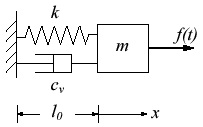
\includegraphics[width=0.90\textwidth]{img/SDOF_plot.png}
    \caption{SDOF system with a linear spring and dashpot}
    \label{fig:SDOF-plot-png}
\end{figure}


\subsection{Equation of Motion for SDOF Systems}

SDOF vibration can be analyzed by \textbf{Newton's second law of motion},
$ F = m a $. The analysis can be easily visualised with the aid of a
\textbf{free body diagram},

\begin{figure}[ht]
    \centering
    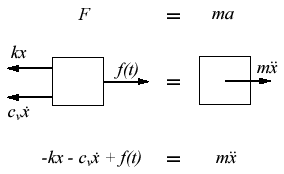
\includegraphics[width=0.90\textwidth]{img/SDOF_FreeBodyDiagram.png}
    \caption{SDOF Free Body Diagram}
    \label{fig:SDOF-freebodydiagram-png}
\end{figure}

The resulting equation of motion is a
\textbf{second order, non-homegeneous, ordinary differential equation}:

\begin{equation}
    m \ddot{u} + c \dot{u} + k u = f(t)
        \left\{ \begin{matrix}
                u(t=0) = u_0\\
                \dot{u}(t=0) = \dot{u}_0
          \end{matrix} \right.
\end{equation}

with the initial conditions $ u_0 $ and $ \dot{u}_0 $.


\subsection{Time Solution for Unforced Undamped SDOF Systems}

\textit{https://www.efunda.com/formulae/vibrations/sdof\_free\_undamped.cfm}

The equation of motion derived in the definition can be simplified to:

\begin{equation}
    m \ddot{u} + k u = 0
        \left\{ \begin{matrix}
                u(t=0) = u_0\\
                \dot{u}(t=0) = \dot{u}_0
          \end{matrix} \right.
\end{equation}

This equation of motion is a
\textbf{second order, homegeneous, ordinary differential equation} (ODE). If the mass
and spring stiffness are constants, the ODE becomes a
\textbf{linear, homogeneous ODE with constant coefficients} and can be solved
by the Characteristic Equation method. The characteristic equation for this
problem is:

\begin{equation}
    m s^2 + k = 0
\end{equation}

which determines the 2 independent roots for the undamped vibration problem.
The final solution (that contains the 2 independent roots from the characteristic
equation and satisfies the initial conditions) is:

\begin{eqarray}
    u(t) &= c_1 e^{i \omega_n t} + c_2 e^{- \omega_n t}\\
         &= d_1 \cos{\omega_n t} + d_2 \sin{\omega_n t} \\
    \implies u(t) &= u_0 \cos{\omega_n t} + \frac{\dot{u}_0}{\omega_n} \sin{\omega_n t}
\end{eqarray}

The natural frequency $ \omega_n $ is defined by:

\begin{equation}
    \omega_n = \sqrt{\frac{k}{m}}
\end{equation}

and depends only on the system mass and the spring stiffness (i.e. any damping will
not change the natural frequency of a system).

Alternatively, the solution may be expressed by the equivalent form,

\begin{equation}
    u(t) = A_0 \cos{(\omega_n t - \phi_0)}
\end{equation}

where the amplitude $ A_0 $ and the intial phase $ \phi_0 $ are given by:

\begin{eqarray}
    A_0 &= \sqrt{u_0^2 + \left(\frac{\dot{u}_0}{\omega_n}\right)^2}\\
    \phi_0 &= \tan^{-1}\frac{\dot{u}_0}{u_0 \omega_n}
\end{eqarray}

\begin{figure}[ht]
    \centering
    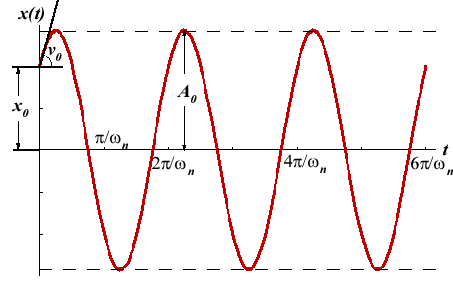
\includegraphics[width=0.90\textwidth]{img/SDOF_Undamped_Response.png}
    \caption{SDOF Undamped sample time behavior}
    \label{fig:SDOF-undamped-response-png}
\end{figure}

Note that an assumption of zero damping is typically not accurate. In reality,
there almost always exists some resistance in vibratory systems. This reistance
will damp the vibration and dissipate energy, the oscillatory motion caused by the
initial disturbance will eventually be reduced to zero.


\subsection{Time Solution for Unforced Damped SDOF Systems}

\textit{https://www.efunda.com/formulae/vibrations/sdof\_free\_damped.cfm}

\begin{figure}[ht]
    \centering
    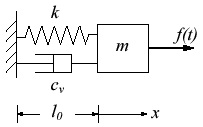
\includegraphics[width=0.90\textwidth]{img/SDOF_plot.png}
    \caption{SDOF system with a linear spring and dashpot}
    \label{fig:SDOF-plot-damped-png}
\end{figure}

Damping that produces a damping force proportional to the mass's velocity is
commonly referred to as \textit{viscous damping}, and is denoted graphically
by a dashpot.

For an unforced damped \textbf{SDOF} system, the general equation of motion
becomes:

\begin{equation}
    m \ddot{u} + c \dot{u} + k u = 0
        \left\{ \begin{matrix}
                u(t=0) = u_0\\
                \dot{u}(t=0) = \dot{u}_0
          \end{matrix} \right.
\end{equation}

Tis equation of motion is a \textbf{second order, homogeneous, ODE}. If all
parameters (mass, stiffness and viscous damping) are constants, the \textbf{ODE}
becomes a \textbf{linear ODE with constant coefficients} and can be solved by
the \textit{Characteristic Equation method}. The characteristic equation for this
problem is:

\begin{equation}
    m s^2 + s_v s + k = 0
\end{equation}

which determines the 2 independent roots for the damped vibration problem.
The roots to the characteristic equation fall into one of the following
3 cases:

\begin{itemize}
    \item If $ c_v^2 - 4 m k < 0 $, the system is termed \textbf{underdamped}.
        The roots of the characteristic equation are complex conjugates,
        corresponding to \textit{oscillatory motion} with an
        \textit{exponential decay} in amplitude.

    \item If $ c_v^2 - 4 m k = 0 $, the system is termed \textbf{critically-derdamped}.
        The roots of the characteristic equation are repeated,
        corresponding to \textit{simple decay motion} with at most
        \textit{one overshoot} of the systems resting position.

    \item If $ c_v^2 - 4 m k > 0 $, the system is termed \textbf{overderdamped}.
        The roots of the characteristic equation are prurely real and distinct,
        corresponding to \textit{simple exponentially decaying motion}.

\end{itemize}

To simplify the solutions coming up, we define the critical damping $ c_c $,
the damping ratio $ \zeta $, and the damped vibration frequency $ \omega_d $ as:

\begin{eqarray}
    c_c &= 2 m \sqrt{\frac{k}{m}} = 2 m \omega_n\\
    \zeta &= \frac{c_v}{c_c}\\
    \omega_d &= \sqrt{1 - \zeta^2} \omega_n
\end{eqarray}

where the natural frequency of the system $ \omega_n $ is given by:

\begin{equation}
    \omega_n = \sqrt{\frac{k}{m}}
\end{equation}

Note that $ \omega_d $ will equal $ \omega_n $ when the damping of the system
is zero (i.e. undamped). The time solutions for the free \textbf{SDOF}
system is presented below for each of the three case scenarios.

\subsubsection{Time Solution of Unforced Underdamped SDOF Systems}

When $ c_v^2 - 4 m k < 0 $ (equivalent to $ \zeta < 1 $ or $ c_v < c_c $),
the characteristic equation has a pair of complex conjugate roots. The displacement
solution for this kind of system is:

\begin{eqarray}
    u(t) &= c_1 e^{-\zeta + i \sqrt{1 - \zeta^2} \omega_n t}
          + c_2 e^{-\zeta - i \sqrt{1 - \zeta^2} \omega_n t}\\
         &= e^{-\zeta \omega_n t} \left[ d_1 \cos{(\omega_d t)}
                                       + d_2 \sin{(\omega_d t)} \right]\\
    \implies u(t) &= \underbrace{e^{-\zeta \omega_n t}}_{exponential\ decay}
    \underbrace{\left[ u_0 \cos{(\omega_d t)}
    + \frac{\dot{u}_0 + \zeta \omega_n u_0}{\omega_d} \sin{(\omega_d t)}
    \right]}_{periodic\ motion}
\end{eqarray}

An alternate but equivalent solution is given by:

\begin{equation}
    u(t) = A_0 \underbrace{e^{-\zeta \omega_n t}}_{exponential\ decay}
    \underbrace{\cos{(\omega_d t - \phi_0)}}_{periodic\ motion}
\end{equation}

\begin{figure}[ht]
    \centering
    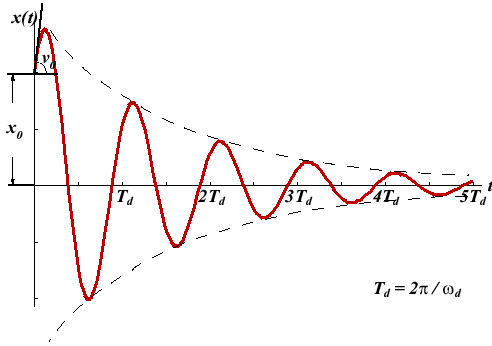
\includegraphics[width=0.70\textwidth]{img/SDOF_UnderDamped_Response.png}
    \caption{The displacement plot of an underdamped system}
    \label{fig:SDOF-underdamped-response-png}
\end{figure}

Note that the displacement amplitude decays exponentially (i.e. the natural
logarithm of the amplitude ratio for any two displacements separated in time
by a constant ratio is a constant):

\begin{eqarray}
    \frac{A_k}{A_{k+1}} &=
    \frac{A_0 e^{-\zeta \omega_n \left( k T_d \right)} \cos{ \left( \phi_0 \right) }}
         {A_0 e^{-\zeta \omega_n \left[ (k+1) T_d \right]} \cos{ \left( \phi_0 \right) }}\\
                        &=
    \frac{e^{-\zeta \omega_n \left( k T_d \right)}}
         {e^{-\zeta \omega_n \left[ (k+1) T_d \right]}}\\
                        &= e^{\zeta \omega_n T_d}\\
    \implies \ln{\left( \frac{A_k}{A_{k+1}} \right)} &=
    \zeta \omega_n T_d = \zeta \omega_n \frac{2 \pi}{\omega_d}
    = \frac{2 \pi \zeta}{\sqrt{1 - \zeta^2}}
\end{eqarray}

where $ T_d = \frac{1}{f_d} = \frac{2 \pi}{\omega_d} $ is the period of the
damped vibration.


\subsubsection{Time Solution of Unforced Critically-Damped Systems}

When $ c_v^2 - 4 m k = 0 $ (equivalent to $ \zeta = 1 $ or $ c_v = c_c $), the
characteristic equation has repeated real roots. The displacement solution for
this kind of system is:

\begin{eqarray}
    u(t) &= \left( c_1 + c_2 t \right) e^{-\omega_n t}\\
    \implies u(t) &= e^{-\omega_n t} \left[ u_0 + \left( v_0 + \omega_n u_0 \right) t \right]
\end{eqarray}

The critical damping factor $ c_c $ can be interpreted as the \textbf{minimum damping}
that results in non-periodic motion (i.e. simple decay).

\begin{figure}[ht]
    \centering
    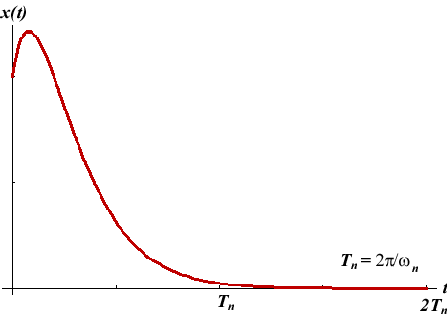
\includegraphics[width=0.70\textwidth]{img/SDOF_CriticalDamped_Response.png}
    \caption{The displacement plot of a critically-damped system with positive initial
displacement and velocity.}
    \label{fig:SDOF-critically-damped-response-png}
\end{figure}

The displacement decays to a negligible level after one natural period $ T_n $.
Note that if the initial velocity $ v_0 $ is negative while the initial displacement
$ u_0 $ is positive, there will exist one overshoot of the resting position in
the displacement plot.


\subsubsection{Time Solution of Unforced Overdamped SDOF Systems}

When $ c_v^2 - 4 m k > 0 $ (equivalent to $ \zeta > 1 $ or $ c_v > c_c $),
the characteristic equation has two distinct real roots. The displacement
solution for this kind of system is:

\begin{eqarray}
    u(t) &= c_1 e^{\left( -\zeta + \sqrt{\zeta^2 - 1} \right) \omega_n t}
          +  c_2 e^{\left( -\zeta - \sqrt{\zeta^2 - 1} \right) \omega_n t}\\
    \implies u(t) &=
    \frac{u_0 \omega_n \left( \zeta + \sqrt{\zeta^2 - 1} \right) + v_0}
    {2 \omega_n \sqrt{\zeta^2 - 1}} e^{\left( -\zeta + \sqrt{\zeta^2 - 1} \right) \omega_n t} +\\
                  &+
    \frac{-u_0 \omega_n \left( \zeta - \sqrt{\zeta^2 - 1} \right) - v_0}
    {2 \omega_n \sqrt{\zeta^2 - 1}} e^{\left( -\zeta - \sqrt{\zeta^2 - 1} \right) \omega_n t}
\end{eqarray}

\begin{figure}[ht]
    \centering
    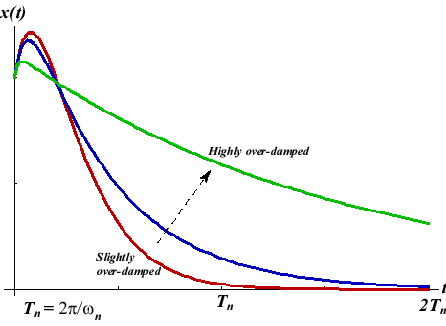
\includegraphics[width=0.70\textwidth]{img/SDOF_OverDamped_Response.png}
    \caption{The displaceent plot of an overdamped system response}
    \label{fig:SDOF-overdamped-response-png}
\end{figure}

The motion of an overdamped system is non-periodic, regardless of the inital conditions.
The larger the damping, the longer time to decay from an initial disturbance.

If the system is heavily damped, $ \zeta \gg 1 $, the displacement solution takes
the approximate form:

\begin{equation}
    u(t) \approx u_0 + \frac{v_0}{2 \zeta \omega_n}
    \left(1 - e^{-2 \zeta \omega_n t} \right)
\end{equation}


\subsection{SDOF Systems under Harmonic Excitaion}
\textit{https://www.efunda.com/formulae/vibrations/sdof\_harmo.cfm}

When a \textbf{SDOF} System is forced by $ f(t) $, the solution for the displacement
$ x(t) $ consists of two parts: the \textit{complimentary solution}, and the
\textit{particular solution}. The complimentary solution for the problem
is given by the \textbf{free vibration of an unforced SDOF System}.
The \textbf{particular solution} depends on the nature fo the forcing function.

When the forcing function is \textbf{harmonic} (i.e. it consits of at most
a \textbf{sine} and \textbf{cosine} at the same \textbf{frequency},
a quantity that can be expressed by the complex exponentional $ e^{i \omega t} $),
the method if \textbf{Undetermined Coefficients} can be used to find the particular
solution. Non-harmonic forcing functions are handled by other techniques.

Consider the SDOF system forced by the harmonic function $ f(t) $.

\begin{figure}[ht]
    \centering
    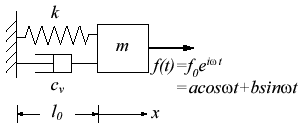
\includegraphics[width=0.70\textwidth]{img/SDOF_harmonic.png}
    \caption{SDOF System forced by the harmonic function $ f(t) $}
    \label{fig:SDOF-harmonic-response-png}
\end{figure}

The particular solution for this problem is found to be:

\begin{equation}
    u_p(t) = \frac{f_0}{ \left( k - m \omega^2 \right) + i c \omega} e^{i \omega t}
\end{equation}

The general solution is given by the sum of the complimentary and particular
solutions multiplied by two weighting constants $ c_1 $ and $ c_2 $,

\begin{equation}
    u(t) = c_1 u_c(t) + c_2 u_p(t)
\end{equation}

The values of $ c_1 $ and $ c_2 $ are found by matching $ u(t=0) $ to the
initial conditions.

\subsubsection{Undamped SDOF Systems under Harmonic Excitation}

For an undamped system ( $ c_v = 0 $ ) the total displacement solution is:

\begin{eqarray}
    u(t) &= d_1 \cos{\omega_n t} + d_2 \sin{\omega_n t} +
    \frac{f_0}{k - m \omega^2} e^{i \omega t}\\
    \implies u(t) &= \left( u_0 - \frac{f_0}{k - m \omega^2} \right) \cos{\omega_n t}\\
                  &+
    \left(\frac{v_0 - \frac{i \omega f_0}{k - m \omega^2}}{\omega_n} \right)
    \sin{\omega_n t}\\
                  &+ \frac{f_0}{k - m \omega^2} e^{i \omega t}
\end{eqarray}

If the forcing frequency is close to the natural frequency, $ \omega \approx \omega_n $,
the system will exhibit \textbf{resonance} (very large displacements) due to
near-zeros in the denominators of $ u(t) $.

When the forcing frequency is equal to the natural frequency, we cannot use the
$ u(t) $ given above as it would give divide-by-zero. Instead we must use
\textbf{L'H\^ospital's Rule} to derive a solution free of zeros in the denominators.

\begin{eqarray}
    u(t) &= u_0 \cos{\omega_n t} + \frac{v_0}{\omega_n} \sin{\omega_n t}\\
         &+ \lim_{\omega \rightarrow \omega_n} \left\{
             \frac{f_0}{k - m \omega^2} \left(
                 e^{i \omega t} - \cos{\omega_n t} - i \omega \sin{\omega_n t}
                 \right)
         \right\}\\
         &= u_0 \cos{\omega_n t} + \frac{v_0}{\omega_n} \sin{\omega_n t}
         - \frac{f_0 \omega_n}{2 k} \left(
             i t e^{i \omega)n t} - i \sin{\omega_n t}
             \right)
\end{eqarray}

To simplify $ u(t) $, let's assume that the driving force consists only of the
cosine function $ f(t) = f_0 \cos{\omega t} $.

\begin{figure}[ht]
    \centering
    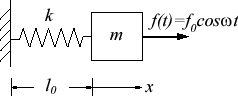
\includegraphics[width=0.35\textwidth]{img/SDOF_harmonic_undamped.png}
    \caption{SDOF System forced by the harmonic function $ f(t) = f_0 \cos{\omega t} $}
    \label{fig:SDOF-harmonic-undamped-response-png}
\end{figure}

The displacement solution reduces to:

\begin{eqarray}
    u(t) &= u_0 \cos{\omega_n t} + \frac{v_0}{\omega_n} \sin{\omega_n t}\\
         &+ \lim_{\omega \rightarrow \omega_n} \left\{
             \frac{f_0}{k - m \omega^2} \left(
                 \cos{\omega t} - \cos{\omega_n t}
                 \right)
         \right\}\\
         &= \underbrace{u_0 \cos{\omega_n t} + \frac{v_0}{\omega_n} \sin{\omega_n t}}_{
         free\ vibration\ (complementary)}
         + \underbrace{\frac{f_0 \omega_n t}{2 k}}_{\Scale[0.75]{
             \begin{matrix}
                 amplitude\\
                 linearly\\
                 increased
             \end{matrix}}}
         \sin{\omega_n t}
\end{eqarray}

This solution contains one term multiplied by $ t $. This term will cause the displacement
amplitude to increase linearly wit time as the forcing function pumps energy into
the system.

\begin{figure}[ht]
    \centering
    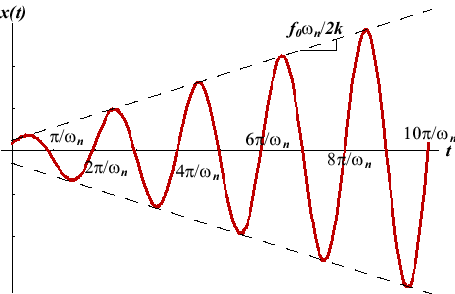
\includegraphics[width=0.70\textwidth]{img/SDOF_Undamped_Harmonic_Response.png}
    \caption{Resonance response of undamped SDOF with harmonic excitation}
    \label{fig:SDOF-undamped-harmonic-response-png}
\end{figure}

The maximum displacement of an undamped system forced at its resonant frequency will
increase unbounded according to the solution for $ u(t) $ above. However, real systems
will inject additional physics once displacements become large enough. These
additional physics (nonlinear plastic deformation, heat transfer, buckling etc.) will
serve to limit the maximum displacement exhibited by the system, and allow one to escape
the "sudden death" impression that such systems will immediately fail.


\subsubsection{Damped SDOF Systems under Harmonic Excitation}

\begin{equation}
    m \ddot{u} + c \dot{u} + k u = F_0 \cos{\left(\omega t \right)}
\end{equation}

then \textbf{steady state} solution is in the form:

\begin{equation}
    u_{s.s.} = u_0 \cos{\left(\omega t - \phi \right)}
\end{equation}

If we plug the \textbf{steady state} solution to the \textbf{equation of motion},
we get:

\begin{eqarray}
    u_o \left[ \left(k - m \omega^2\right) \cos{\omega t - \phi} -
    c \omega \sin{\left( \omega t - \phi \right)} \right]
    &= F_0 \cos{\left( \omega t \right)} \quad \vert \times \frac{1}{k}\\
        u_o \left[ \left(1 - \frac{\omega^2}{\omega_n^2} \right) \cos{\omega t - \phi} -
        2 \zeta \frac{\omega}{\omega_n} \sin{\left( \omega t - \phi \right)} \right]
    &= \frac{F_0}{k} \cos{\left( \omega t \right)}
\end{eqarray}

because:
\begin{equation}
    \frac{k}{m} = \omega_n
\end{equation}

\begin{equation}
    \zeta = \frac{c}{c_c}
\end{equation}

\begin{equation}
    c = 2 m \sqrt{\frac{k}{m}} = 2 m \omega_n
\end{equation}

\begin{equation}
    \frac{c}{k} = \frac{\zeta c_c}{k} = \frac{\zeta 2 m \omega_n}{k}
    = \frac{2 \zeta \omega_n^2}{omega_n^2} = \frac{2 \zeta}{\omega_n}
\end{equation}

after utilising the sine and cosine relations:

\begin{eqarray}
    \cos{\left( \omega t - \phi \right)} &=
    \cos{\omega t} \cos{\phi} + \sin{\omega t} \sin{\phi}\\
    \sin{\left( \omega t - \phi \right)} &=
    \sin{\omega t} \cos{\phi} + \cos{\omega t} \sin{\phi}
\end{eqarray}

we get a set of two equatons:
\begin{eqarray}
    u_o \left[ \left(1 - \frac{\omega^2}{\omega_n^2} \right) \cos{\phi} +
    2 \zeta \frac{\omega}{\omega_n} \sin{\phi} \right] \cos{\omega t}
    &= \frac{F_0}{k} \cos{\left( \omega t \right)}\\
    u_o \left[ \left(1 - \frac{\omega^2}{\omega_n^2} \right) \sin{\phi} -
    2 \zeta \frac{\omega}{\omega_n} \cos{\phi} \right] \sin{\omega t}
    &= 0\\
\end{eqarray}

and when solving just for amplitudes this reduces to a set of two algebraic equations
which is then solved for $ u_0 $ and $ \phi $:
\begin{eqarray}
    u_o \left[ \left(1 - \frac{\omega^2}{\omega_n^2} \right) \cos{\phi} +
    2 \zeta \frac{\omega}{\omega_n} \sin{\phi} \right]
    &= \frac{F_0}{k}\\
    u_o \left[ \left(1 - \frac{\omega^2}{\omega_n^2} \right) \sin{\phi} -
    2 \zeta \frac{\omega}{\omega_n} \cos{\phi} \right]
    &= 0\\
\end{eqarray}

The solution (\textbf{transfer function}) is finally:
\begin{eqarray}
    u_0 &= \frac{\frac{F_0}{k}}{
        \left[
            \left( 1 - \frac{\omega^2}{\omega_n^2} \right)^2 +
            \left( 2 \zeta \frac{\omega}{\omega_n} \right)^2
    \right]^{\frac{1}{2}}}\\
    \phi &= \tan^{-1} \left(
        \frac{2 \zeta \frac{\omega}{\omega_n}}{
    1 - \frac{\omega^2}{\omega_n^2}} \right)
\end{eqarray}

where:\\
$ u_0 $ is displacement amplitude\\
$ \frac{F_0}{k} $ is displacement from static simulation.

\begin{equation}
    H_0 = \frac{\frac{F_0}{k}}{
        \left[
            \left( 1 - \frac{\omega^2}{\omega_n^2} \right)^2 +
            \left( 2 \zeta \frac{\omega}{\omega_n} \right)^2
    \right]^{\frac{1}{2}}}
\end{equation}





\newpage
\section{Damping}

\subsection{Rayleigh Damping}
\textit{https://www.simscale.com/knowledge-base/rayleigh-damping-coefficients/}

Let \textbf{Rayleigh Damping} be defined as:

\begin{equation}
    c = \alpha k + \beta m
\end{equation}

where:\\
$ c $ is damping value [-],\\
$ \alpha $ is stiffness dependent damping coefficient,\\
$ \beta $ is inertia (mass) dependent damping coefficient,\\
$ m $ is mass and\\
$ k $ is stiffness.

Thus, substituting this relation to the equation of motion:

\begin{eqarray}
    m \ddot(u) + \left(\alpha k + \beta m \right) \dot{u} + k u &= f(t) & \space \vert \times \frac{1}{m}\\
    \ddot{u} + \left(\alpha \frac{k}{m} + \beta \frac{m}{m} \right) \dot{u} + \frac{k}{m} u
    &= \frac{f(t)}{m} & \space \vert \frac{k}{m} = \omega_n^2 \\
    \ddot{u} + \left(\alpha \omega_n^2 + \beta \right) \dot{u} + \omega_n^2 u &= \frac{f(t)}{m} & \space
\end{eqarray}

Damping Ratio:

\begin{eqarray}
    \zeta &= \frac{c}{2 m \omega_n}\\
    \zeta &= \frac{1}{2 m \omega_n} \left( \alpha k + \beta m \right)\\
    \zeta &= \frac{1}{2} \left( \alpha \omega_n + \frac{\beta}{\omega_n} \right)
\end{eqarray}

where:\\
$ \zeta $ is damping ratio,\\
$ c $ is damping value [-],\\
$ m $ is mass and\\
$ \omega_n $ is natural frequency [rad/s]

Substituting back:

\begin{equation}
    \ddot{u} + 2 \zeta \omega_n \dot{u} + \omega_n^2 k u = \frac{f(t)}{m}
\end{equation}


When \textbf{Damping is proportional to inertia}:

In this case, the stiffness coefficient $ \alpha = 0 $ and thus:

\begin{equation}
    \zeta = \frac{\beta}{2 \omega_n}
\end{equation}

For a given constant value of $ \beta $, it is seen that the damping is inversely
proportional to the natural frequency, as shown in the illustration:

\begin{figure}[ht]
    \centering
    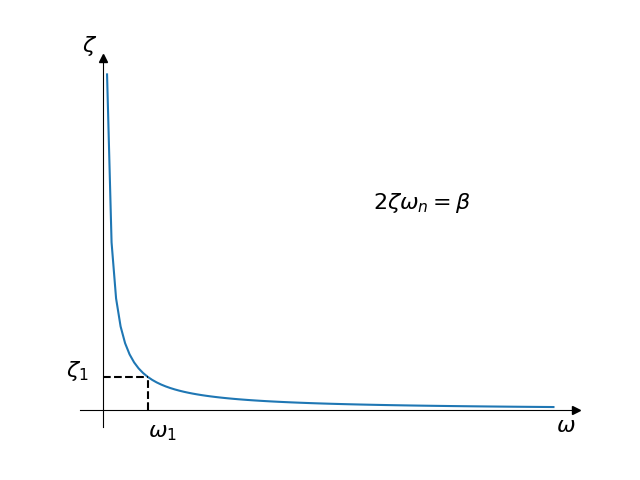
\includegraphics[width=0.90\textwidth]{img/inertia_dependent_damping.png}
    \caption{Schematic of damping proportional to inertia}
    \label{fig:inertia-dependent-damping-png}
\end{figure}

Moreover, if one computes $ \beta $ from the damping ration $ \zeta_1 $ at a given
natural frequency $ \omega_1 $, all the natural frequencies below it will be amplified
and the frequencies above it will be attenuated. The effect is more dramatic the farther
the frequencies are from the reference value.

When \textbf{Damping is proportional to stiffness}:

In this case, the mass coefficient $ \beta = 0 $ and thus:

\begin{equation}
    \zeta = \frac{1}{2} \alpha \omega_n
\end{equation}

It is seen that, contrary to the first case, here the damping id directly proportional
to the natural frequency:

\begin{figure}[ht]
    \centering
    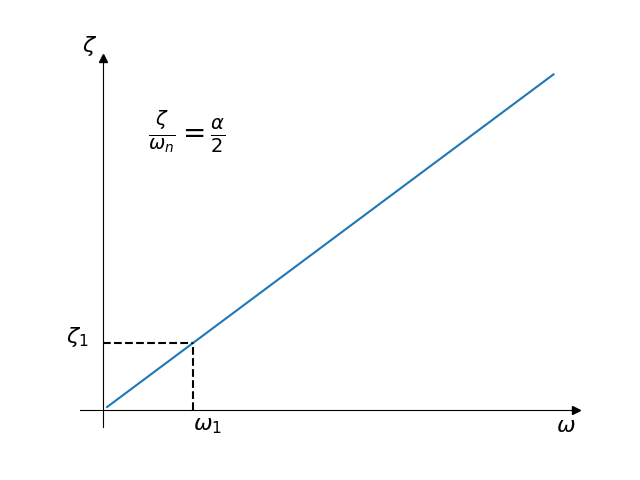
\includegraphics[width=0.90\textwidth]{img/stiffness_dependent_damping.png}
    \caption{Schematic of damping proportional to stiffness}
    \label{fig:stiffness-dependent-damping-png}
\end{figure}

If one computes $ \alpha $ from the damping ratio $ \zeta_1 $ at a natural
frequency $ \omega_1 $, then the natural frequencies below will be attenuated and
the frequencies above will be amplified.

\textbf{General Case}:

In the case of using the model with two parameters, the proportionality of damping
against frequency is convex:

\begin{figure}[ht]
    \centering
    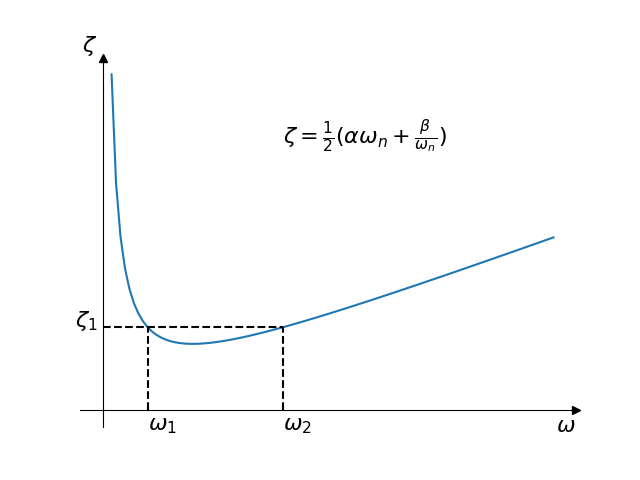
\includegraphics[width=0.90\textwidth]{img/general_rayleigh_damping.png}
    \caption{Schematic of full damping model}
    \label{fig:general-rayleigh-damping-png}
\end{figure}

In this case one needs two damping ratios and two natural frequencies to create
a pair of equations and solve for $ \alpha $ and $ \beta $. The model gives some
flexibility on where to place the natural frequencies, but in general, frequencies
too far away from the ones used in the computation will be amplified.

In the particular case of using equal damping ratios for the two frequencies,
it is important to note that the damping ratio \textbf{will not be constant inside the range}
defined by the sample points, but the inner frequencies will be attenuated. That is,
the inner frequencies will have a lower damping ratio.

\textbf{Computing the Rayleigh Damping Coefficients}

In the most common case, a transient response curve frim the system is obtained and
the damping ratio $ \zeta_1 $ is determined for the lowest natural frequency
$ \omega_1 $ by measuring the (logarithmic) attenuation of successive peaks.

\begin{figure}[ht]
    \centering
    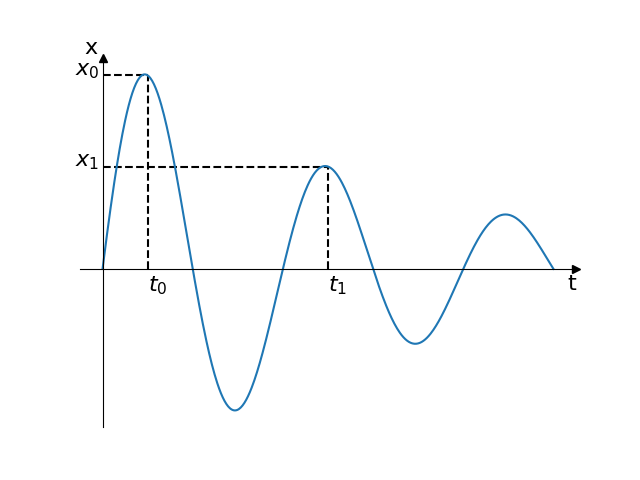
\includegraphics[width=0.90\textwidth]{img/Logarithmic_Decay_Damping_Ratio.png}
    \caption{Determination of the damping ration from the logarithmic decay}
    \label{fig:logarithmic-decay-damping-ratio-png}
\end{figure}

\begin{eqarray}
    \zeta &= \frac{\delta}{\sqrt{\delta^2 + (2 \pi)^2}}\\
    \delta &= \ln{\frac{x_0}{x_1}}\\
    f &= \frac{1}{T} = \frac{1}{t_1 - t_0}\\
    \omega &= 2 \pi f
\end{eqarray}

It is then most common to assume the case of damping proportional to the stiffness,
that is, $ \beta = 0 $, and the $ \alpha $ stiffness coefficient is computed from:

\begin{equation}
    \alpha = \frac{2 \zeta_1}{\omega_1} = \frac{\zeta+1}{\pi f_1}
\end{equation}

If the knowledge on the system indicates the case of damping decreasing with the
frequency, then one can assume the case of damping proportional to the inertia,
where $ \alpha = 0 $ and determine the mass coefficient $ \beta $:

\begin{equation}
    \beta = 2 \zeta_1 \omega_1 = 4 \pi \zeta_1 f_1
\end{equation}

If there is not such test data or knowledge of the system, or if one wishes to apply
an approximate damping ration over a range of frequencies, then we can use the
general case and build a system of two equations:

\begin{eqarray}
    \zeta_1 &= \frac{1}{2} \left( \alpha \omega_1 + \frac{\beta}{\omega_1} \right)\\
    \zeta_2 &= \frac{1}{2} \left( \alpha \omega_2 + \frac{\beta}{\omega_2} \right)
\end{eqarray}

Then solve for the unknown coefficients, keeping in mint the considerations given
above for the general case and the influence of the model on natural frequencies
inside and outside the range of interest. That is, perhaps one wants to achieve
a mean damping ratio over the range, then compensate the attenuation by modifying
the input damping rations, or by performing some least-squares approximation from
more than two frequency points.







\newpage
\section{Modal decomposition}

\subsection{Definition}

Let:

\begin{equation}
    \m{M}\ddot{\m{u}} + \m{C}\dot{\m{u}} +  \m{K}\m{u} = \m{F}\left( t \right)
\end{equation}

be the \textbf{equation of motion}, then:\\
$ \M{\Lambda} $ is a \textbf{spectral} matrix\\
$ \M{\Psi} $ is a \textbf{mode shape} matrix,

such that:
\begin{equation}
    \M{\Lambda} =
    \begin{bmatrix}
        \lambda_1^2 & \dots & 0\\
        \vdots & \ddots & \vdots \\
        0 & \dots & \lambda_n^2
    \end{bmatrix}
\end{equation}

where $ \lambda_n^2 $ is the n-th eigenvalue of the problem
$ (\m{K}-\lambda^2\m{M})\m{X} = 0 $

and:
\begin{equation}
    \M{\Psi} =
    \begin{bmatrix}
        \M{\psi}_1 & \dots & \M{\psi}_n
    \end{bmatrix}
\end{equation}

where $ \M{\psi}_n = \{\psi_{n,1}, \dots, \psi_{n,m}\}^T $ is the eigenvector
of the n-th eigenvalue $ \lambda_n^2 $.

The \textbf{displacement} $ \m{u} $ can be expressed as a linear combination
of eigenvectors such that:

\begin{eqarray}
    \m{u}(t)
    &= \M{\Psi} \m{q}(t) \\
    &= \begin{bmatrix}
        \M{\psi}_1 & \dots & \M{\psi}_n
    \end{bmatrix} \m{q}(t) \\
    &= \begin{bmatrix}
        \M{\psi}_{1,1} & \dots & \M{\psi}_{n,1} \\
        \vdots & \vdots & \vdots \\
        \M{\psi}_{1,m} & \dots & \M{\psi}_{n,m}
    \end{bmatrix}
    \begin{bmatrix}
        q_1(t) \\
        \vdots \\
        q_n(t)
    \end{bmatrix}
\end{eqarray}

where $ \m{q}(t) $ is a vector of modal coefficients.

Then:

\begin{eqarray}
    \dot{\m{u}}(t) &= \M{\Psi} \dot{\m{q}}(t) \\
    \ddot{\m{u}}(t) &= \M{\Psi} \ddot{\m{q}}(t)
\end{eqarray}

First we substitute $ \m{u} = \M{\Psi}\m{q} $ to the
\textbf{equation of motion}:

\begin{equation}
    \m{M} \M{\Psi} \ddot{q} +
    \m{C} \M{\Psi} \dot{q} +
    \m{K}\M{\Psi}\m{q}
    = \m{F}(t)
\end{equation}

By \textbf{premultiplying} with $ \M{\Psi}^T $ we get:

\begin{equation}
    \M{\Psi}^T \m{M} \M{\Psi} \ddot{\m{q}} +
    \M{\Psi}^T \m{C} \M{\Psi} \dot{\m{q}} +
    \M{\Psi}^T \m{K} \M{\Psi} \m{q} =
    \M{\Psi}\m{F}(t) = \m{Q}(t)
\end{equation}

where $ \m{Q}(t) = \M{\Psi} \m{F}(t) $ is called a \textbf{modal load}.

\subsection{Orthonormalised Modal Base}

Then one can exploit the properties of \textbf{orthonormalised eigenvectors}, where:

\begin{equation}
    \M{\psi}_r^T \M{\psi}_s = 0 \Leftrightarrow r \neq s
\end{equation}

The \textbf{mass}, \textbf{damping} and \textbf{stiffness} matrices are therefore
reduced to:

\begin{eqarray}
    \M{\Psi}^T \m{M} \M{\Psi}
    &= \begin{bmatrix}
        m_1 & \dots & 0 \\
        \vdots & \ddots & \vdots \\
        0 & \dots & m_n
    \end{bmatrix} \\
    \M{\Psi}^T \m{C} \M{\Psi}
    &= \begin{bmatrix}
        c_1 & \dots & 0 \\
        \vdots & \ddots & \vdots \\
        0 & \dots & c_n
    \end{bmatrix} \\
    \M{\Psi}^T \m{K} \M{\Psi}
    &= \begin{bmatrix}
        k_1 & \dots & 0 \\
        \vdots & \ddots & \vdots \\
        0 & \dots & k_n
    \end{bmatrix}
\end{eqarray}

where: \\
$ m_i $ is the \textbf{modal mass} of the i-th shape\\
$ c_i $ is the \textbf{modal damping} of the i-th shape\\
$ k_i $ is the \textbf{modal stiffness} of the i-th shape

\begin{bbox}[0.96]
    \textbf{Note}:

    When are the eigenvectors \textbf{orthonormalised} to \textbf{mass}, the above
    equations reduce to:

    \begin{eqarray}
        \M{\Psi}^T \m{M} \M{\Psi}
        &= \begin{bmatrix}
            1.0 & \dots & 0 \\
            \vdots & \ddots & \vdots \\
            0 & \dots & 1.0
        \end{bmatrix} = \m{I} \\
        \M{\Psi}^T \m{C} \M{\Psi}
        &= \begin{bmatrix}
            c_1 & \dots & 0 \\
            \vdots & \ddots & \vdots \\
            0 & \dots & c_n
        \end{bmatrix} \\
        \M{\Psi}^T \m{K} \M{\Psi}
        &= \begin{bmatrix}
            \lambda_1^2 & \dots & 0 \\
            \vdots & \ddots & \vdots \\
            0 & \dots & \lambda_n^2
        \end{bmatrix} = \M{\Lambda}^2
    \end{eqarray}

    \textbf{Mass normalisation}:

    \begin{equation}
        \M{\psi}_{i,mass} = \frac{\M{\psi}_i}{\M{\psi}_i^T \m{m}_i \M{\psi}_i}
    \end{equation}

    where:

    $ \m{m}_i $ is the i-th row of the \textbf{mass} matrix $ \m{M} $.

\end{bbox}


\subsection{MDOF to SDOF}

The MDOF \textbf{equation of motion} can be then rewritten as a set of \textbf{SDOF}
equations:

\begin{eqarray}
    \M{\Psi}^T \m{M} \M{\Psi} \ddot{\m{q}}(t) +
    \M{\Psi}^T \m{C} \M{\Psi} \dot{\m{q}}(t) +
    \M{\Psi}^T \m{K} \M{\Psi} \m{q}(t) &=
    \M{\Psi}^T \m{F}(t) \\
    \m{M}_{\Psi} \ddot{\m{q}}(t) +
    \m{C}_{\Psi} \dot{\m{q}}(t) +
    \m{K}_{\Psi} \m{q}(t) &= \m{Q}(t)
\end{eqarray}

Written explicitely:

\begin{eqarray}
    \begin{bmatrix}
        m_1 & \dots & 0 \\
        \vdots & \ddots & \vdots \\
        0 & \dots & m_n
    \end{bmatrix}
    \begin{bmatrix}
        \ddot{q}_1(t) \\
        \vdots \\
        \ddot{q}_n(t)
    \end{bmatrix} &+ \\
    \begin{bmatrix}
        c_1 & \dots & 0 \\
        \vdots & \ddots & \vdots \\
        0 & \dots & c_n
    \end{bmatrix}
    \begin{bmatrix}
        \dot{q}_1(t) \\
        \vdots \\
        \dot{q}_n(t)
    \end{bmatrix} &+ \\
    \begin{bmatrix}
        k_1 & \dots & 0 \\
        \vdots & \ddots & \vdots \\
        0 & \dots & k_n
    \end{bmatrix}
    \begin{bmatrix}
        q_1(t) \\
        \vdots \\
        q_n(t)
    \end{bmatrix} &=
    \begin{bmatrix}
        Q_1(t) \\
        \vdots \\
        Q_n(t)
    \end{bmatrix}
\end{eqarray}

It is important to note that all modal matrices (mass, damping and stiffness) are
purely diagonal (with simple enough damping), so the \textbf{MDOF} problem reduces to a series
of \textbf{SDOF} problems:

\begin{eqarray}
    m_1 \ddot{q}_1(t) + c_1 \dot{q}_1(t) + k_1 q_1(t) &= Q_1(t) \\
    m_2 \ddot{q}_2(t) + c_2 \dot{q}_2(t) + k_2 q_2(t) &= Q_2(t) \\
    \vdots \\
    m_n \ddot{q}_n(t) + c_n \dot{q}_n(t) + k_n q_n(t) &= Q_n(t)
\end{eqarray}

which are solved separately and the results are \textbf{linearly} combined:

\begin{eqarray}
    \m{u} = \sum_{i=1}^n \M{\psi}_i q_i \\
    \m{\dot{u}} = \sum_{i=1}^n \M{\psi}_i \dot{q}_i \\
    \m{\ddot{u}} = \sum_{i=1}^n \M{\psi}_i \ddot{q}_i
\end{eqarray}

\begin{bbox}[0.96]
    \textbf{Note:} Above equation can be also written as:

    \begin{eqarray}
        \m{u} = \sum_{i=1}^n \M{\psi}_i q_{u,i} \\
        \m{v} = \sum_{i=1}^n \M{\psi}_i q_{v,i} \\
        \m{a} = \sum_{i=1}^n \M{\psi}_i q_{a,i}
    \end{eqarray}

    where:\\
    $ \m{u} $ is displacement \\
    $ \m{v} $ is velocity \\
    $ \m{a} $ is acceleration

    and\\
    $ \m{q}_{u} $ is modal displacement \\
    $ \m{q}_v $ is modal velocity \\
    $ \m{q}_a $ is modal acceleration

\end{bbox}


\subsection{Initial Conditions}

To get the initial modal conditions, one simply:

\begin{eqarray}
    \m{q}_0 &= \M{\Psi}^{-1} \m{u}_0 \\
    \m{\dot{q}}_0 &= \M{\Psi}^{-1} \m{\dot{u}}_0 \\
    \m{\ddot{q}}_0 &= \M{\Psi}^{-1} \m{\ddot{u}}_0
\end{eqarray}

where:\\
$ \M{\Psi}^{-1} $ is an inverse of eigenshape matrix $ \Leftrightarrow $ all eigenvalues
and eigenshapes are used.

\begin{bbox}[0.96]
    \textbf{Note}: This is not usually so. Normally one would use
    \textbf{reduced modal base}, where only the first \textbf{n} eigenmodes are used. Then
    $ \M{\Psi}^{-1} $ is written as $ \M{\Psi}^{+} $ and called the
    \textbf{pseudoinverse of mode shape matrix} defined (at least in \textbf{numpy}
    - \textit{numpy.linal.pinv()}) as:\\

    \smallskip
    The pseudo-inverse of a matrix $ \m{A} $, denoted $ \m{A}^{+} $,
    is defined as: “the matrix that ‘solves’ [the least-squares problem]
    $ \m{A} \m{x} = \m{b} $ ,” i.e., if $ \overline{\m{x}} $
    is said solution, then $ \m{A}^{+} $ is that matrix such that
    $ \overline{\m{x}} = \m{A}^{+} \m{b} $.\\

    \smallskip
    It can be shown that if $ \m{Q}_1 \M{\Sigma} \m{Q}_2^T = \m{A} $
    is the singular value decomposition of $ \m{A} $, then
    $ \m{A}^{+} = \m{Q}_2 \M{\Sigma}^{+} \m{Q}_1^T $, where $ \m{Q}_{1,2} $
    are orthogonal matrices, $ \M{\Sigma} $  is a diagonal matrix consisting of
    $ \m{A} $’s so-called singular values, (followed, typically, by zeros),
    and then $ \M{\Sigma}^{+} $ is simply the diagonal matrix consisting
    of the reciprocals of $ \m{A} $’s singular values (again, followed
    by zeros).
\end{bbox}



\chapter{Kinematics}
\section{Rigid Body Motion}

A rigid freebody relation between \textbf{slave} (dependent) and \textbf{master}
(independent) DOFs is calculated following the equation:

\begin{eqarray}\label{freebody-master-slave}
    \m{T}_s &= \m{T}_m + \m{R}_s \times \m{x}\\
    \m{R}_s &= \m{R}_m
\end{eqarray}

where
$ \m{T} $ is a translations vector
$ = \left\{ \m{T}_1, \m{T}_2,  \m{T}_3 \right\} $,
$ \m{R} $ is a rotations vector
$ = \left\{ \m{R}_1, \m{R}_2,  \m{R}_3 \right\} $,
$ \m{x} $ is a vector from slave (base) to the master node (tip)
$ = \left\{ \m{x}_s - \m{x}_m,  \m{y}_s - \m{y}_m,
\m{z}_s - \m{z}_m \right\} $ and
$ \times $ is a vector (cross) product.



\chapter{Iterative Methods}

\section{second order ODE's}

Most of FEM problems are \textbf{second order Ordinary Differential Equations}, e.g:

\begin{eqarray}
    m \frac{u''(t)}{d^2 t} + c \frac{u'(t)}{dt} + k u(t) &= 0\\
    m \ddot{u} + c \dot{u} + k u &= 0\\
    m a + c v + ku &= 0
\end{eqarray}

while the iterative methods are for \textbf{first order ODE's} only.
A \textbf{substitution} technique is therefore used to transform the
\textbf{second order ODE's} to a set of \textbf{first order ODE's} and these are
then solved sequentialy.

First we begin with a \textbf{second order ODE} in the form of:

\begin{equation}
    a \frac{y''(x)}{d^2 x} + b \frac{y'(x)}{dx} + c y = d, \quad with \quad y(0) = y_0 \quad and \quad
    \frac{y'(0)}{dx} = y_1
\end{equation}

By stating:

\begin{equation}
    \frac{dy}{dx} = z
\end{equation}

and substituting back:

\begin{equation}
    a \frac{dz}{dx} + b z + c y = d
\end{equation}

now we can write the following set of equations:

\begin{eqarray}
    \begin{aligned}
        z &= \frac{dy}{dx}\\
        \frac{dz}{dx} &= \frac{d - c y - b z}{a}
    \end{aligned} &
    \quad \left\{
    \begin{aligned}
        y(0) &= y_0\\
        z(0) &= y_1
    \end{aligned} \right.
\end{eqarray}



\section{Explicit}

\subsection{Euler's method}
The \textbf{Euler's Method} is an iterative method to solve ODEs. This method's
huge plus is it is fast. The minus is it gradually diverges from the ideal solution.

The \textbf{Euler's Method} uses the following formula:

\begin{equation}
    y(t + h) = y(t) + h f(x,y)
\end{equation}

to construct the tangent at point $ x $ and obtain the value of $ y(x + h) $,
whose slope is:

\begin{equation}
    f(x,y) \quad or \quad \frac{dy}{dx}
\end{equation}

\begin{figure}[ht]
    \centering
    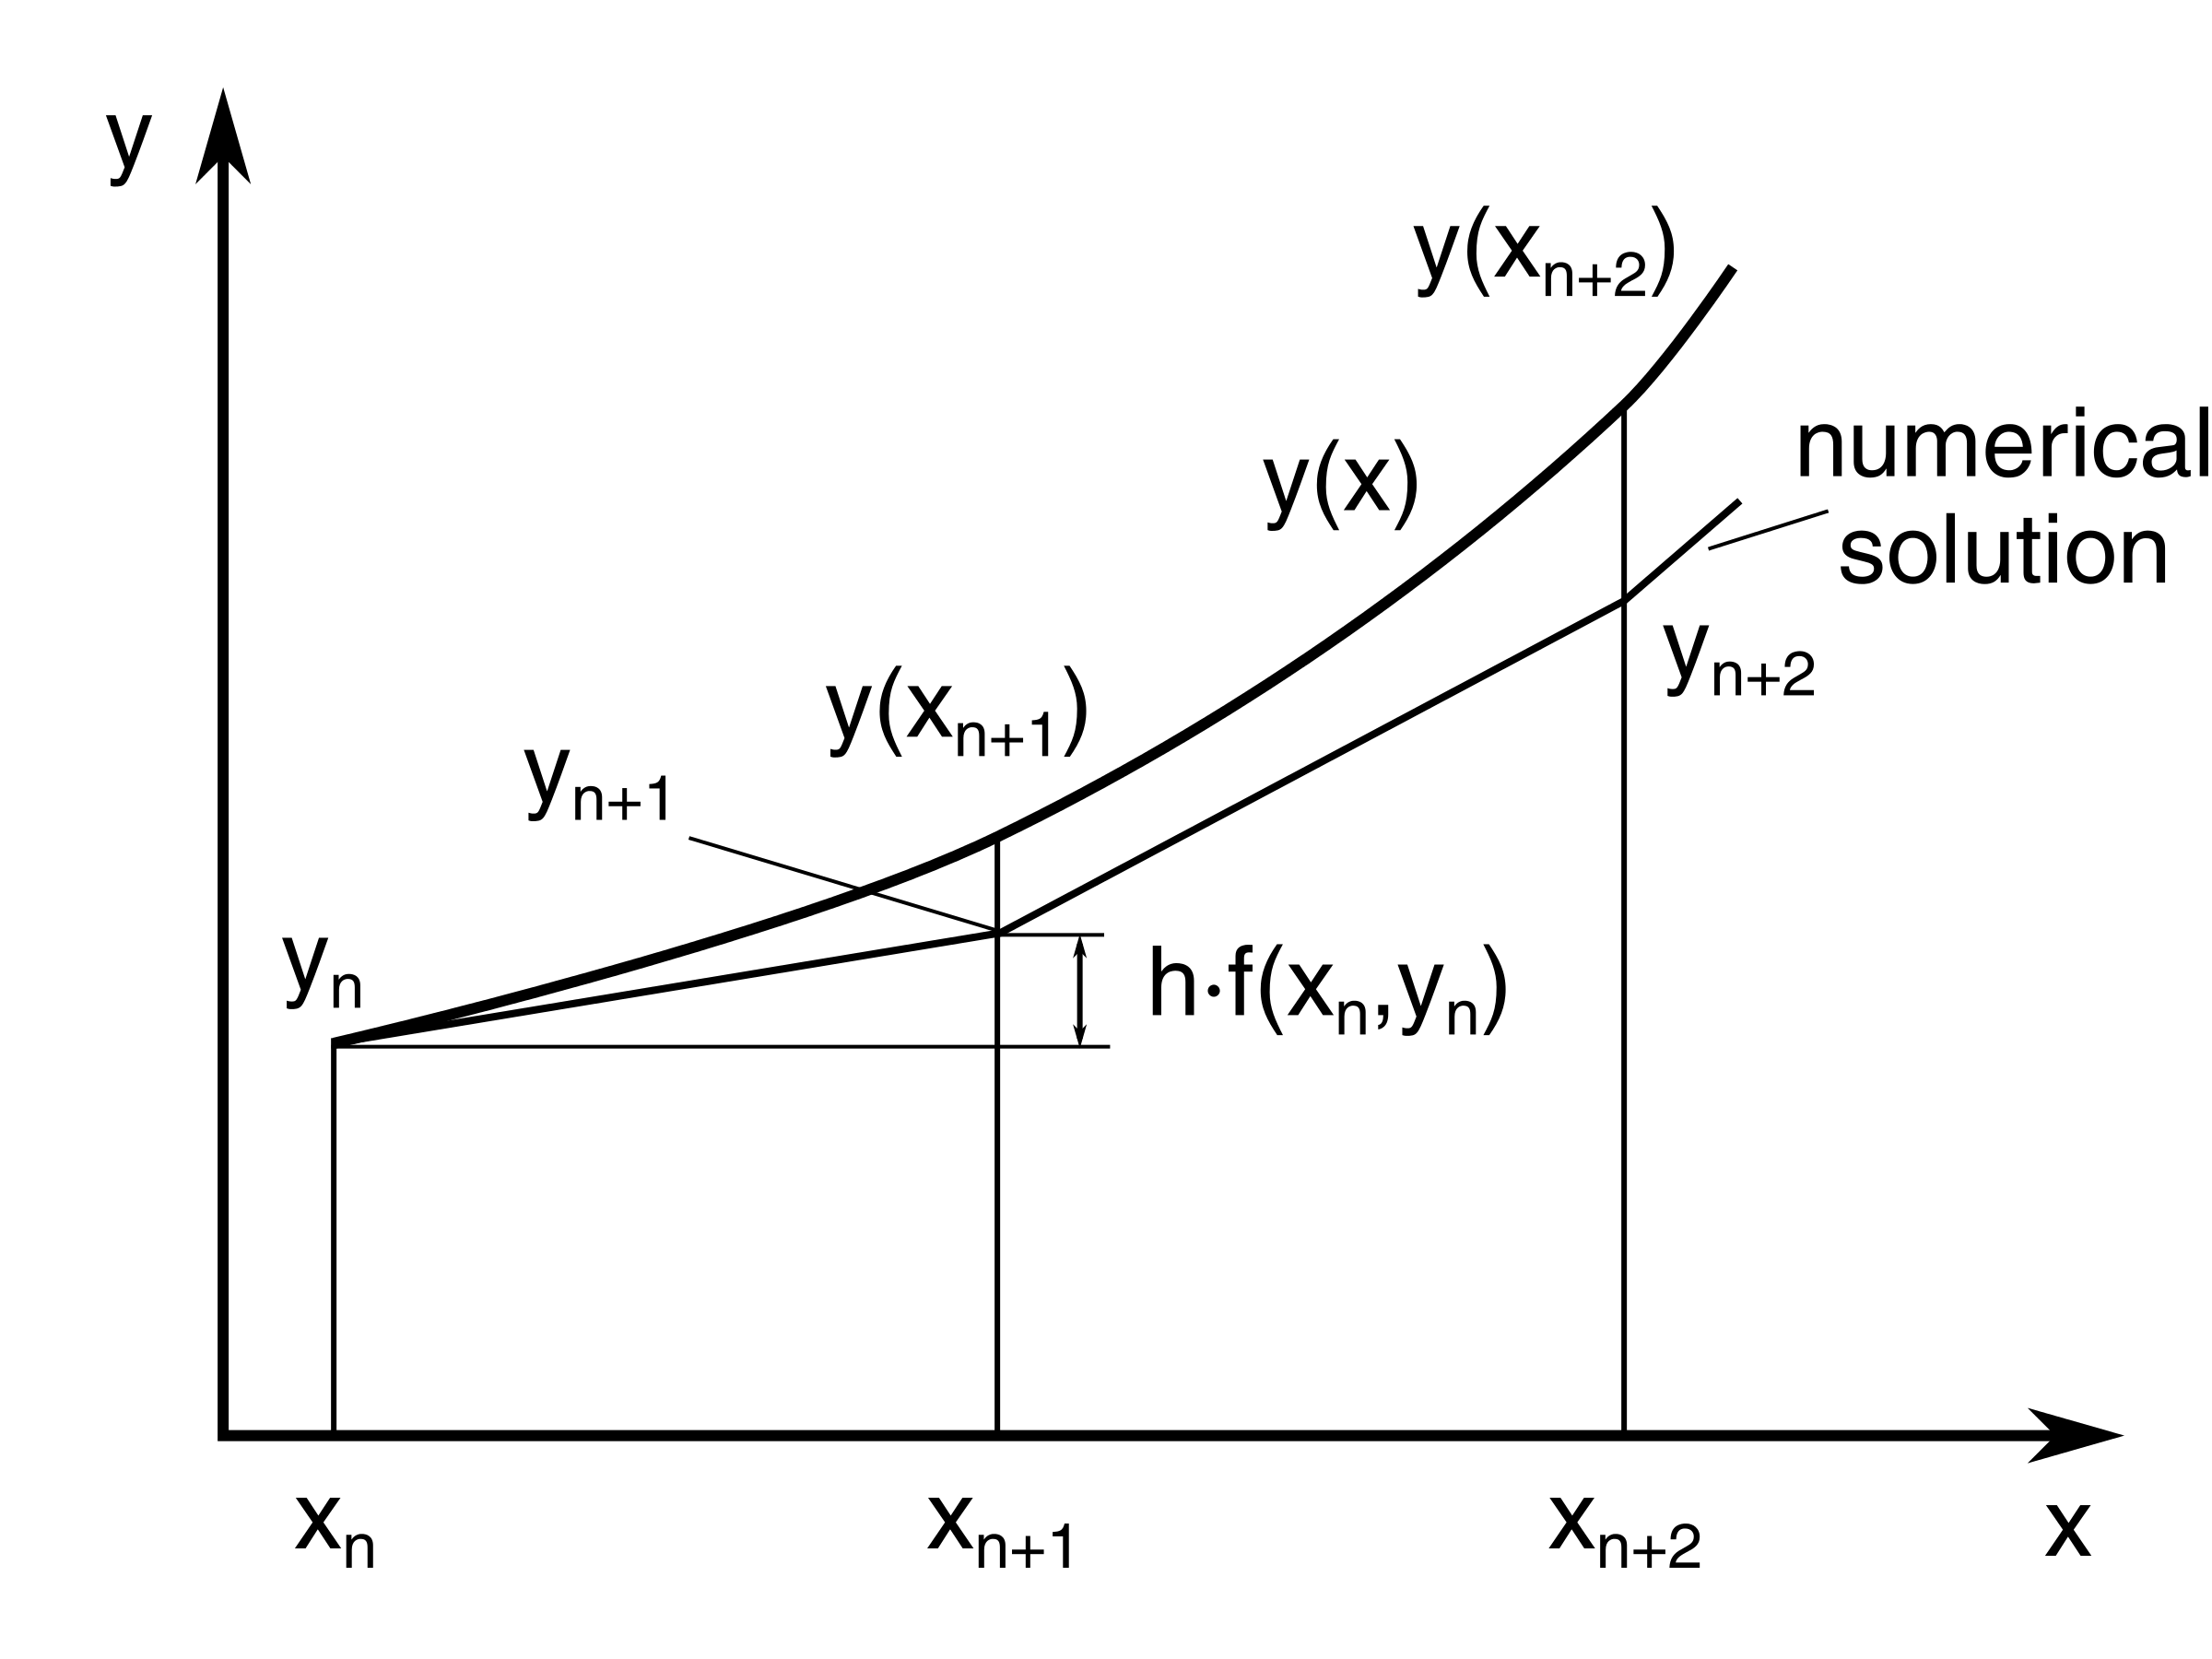
\includegraphics[width=0.90\textwidth]{img/Euler.png}
    \caption{Euler's method schematic}
    \label{fig:euler-png}
\end{figure}

In Euler's method, you can approximate the curve of the solution byt the tangent
in each interval (that is, by a sequence of shor line segments), at steps of $ h $.

\textit{In general}, if you use small step size, the accuracy of the approximation
increases.

\textbf{General Formula}

\begin{equation}
    y_{i+1} = y_i + h f(x_i,y_i)
\end{equation}

where:\\
$ y_{i+1} $ is the next estimated solution value,\\
$ y_i $ is the current value,\\
$ h $ is the interval between steps and\\
$ f(x_i,y_i) $ is the value of the derivative at the current $ (x_i,y_i) $ point.

\textbf{Pseudocode:}

\begin{itemize}
    \item define: $ f(x,y) $

    \item input: $ x_0 $, $ y_0 $

    \item input: $ h $, $ n $

    \item for $ j $ from $ 0 $ to $ (n-1) $ do
        \begin{itemize}
            \item $ y_{j+1} = y_j + hf(x_j, y_j) $
            \item $ x_{j+1} = x_j + h $
            \item Print $ x_{j+1} $ and $= y_{j+1} $
        \end{itemize}
    \item End.
\end{itemize}


\begin{bbox}[0.96]
\textbf{Note:}

If thinking about a problem in time domain:

\begin{itemize}
    \item define: $ f(t,x) $

    \item input: $ t_0 $, $ x_0 $

    \item input: $ dt $, $ n $

    \item for $ j $ from $ 0 $ to $ (n-1) $ do
        \begin{itemize}
            \item $ x_{j+1} = x_j + dt f(t_j, x_j) $
            \item $ t_{j+1} = t_j + dt $
            \item Print $ t_{j+1} $ and $= x_{j+1} $
        \end{itemize}
    \item end.
\end{itemize}

\end{bbox}


\newpage
\textbf{Python Code for vibration problem:}

\begin{python}
#!/usr/bin/python3
import numpy as np
import matplotlib.pyplot as plt


def iterate(h, y0, func, rhs):
    num_of_odes = y0.shape[0]
    y1 = np.zeros(num_of_odes, dtype = float)
    for i in range(num_of_odes-1):
        y1[i] = y0[i] + y0[i+1] * h
    y1[-1] = func(y1, rhs)
    return y1


def euler(t, y, func, rhs):
    N = t.shape[0]
    for j in range(N-1):
        dt = t[j+1] - t[j]
        y[j+1,:] = iterate(dt, y[j,:], func, rhs[j])
        # print(y[j+1,:])
    return y


def euler_vibration():
    m = 0.55  # tonnes
    c = 3.    # Ns/mm
    k = 1000. # N/mm

    freq = np.sqrt(k / m) / (2 * np.pi)

    # equation to solve
    # m * a + c * v + k * u = f
    # a = (f - c * v - k * u) / m
    acceleration = lambda u, f: (f - c * u[1] - k * u[0]) / m

    T = 2.0     # seconds
    dt = 0.0001 # timestep s
    u_0 = 0.    # mm of initial displacement
    v_0 = 0.    # mm/s of initial velocity

    # times at which to solve
    t = np.linspace(0, T, int(T/dt) + 1)

    # force vector
    F = 5000. # N of max impulse
    t0 = 0.1  # impulse start time
    t1 = 0.2  # impuls end time
    f = np.zeros(t.shape[0], dtype=float)
    # create a half sine impulse of force
    for i in range(t.shape[0]):
        if t[i] >= t0 and t[i] <= t1:
            f[i] = F * np.sin((t[i] - t0) / (t1 - t0) * np.pi)
        else:
            f[i] = 0.

    uva = np.zeros((t.shape[0],3), dtype=float)
    uva[0,0] = u_0
    uva[0,1] = v_0

    uva = euler(t, uva, acceleration, f)

    fig, axf = plt.subplots()
    fig.subplots_adjust(right=0.60)

    p1, = axf.plot(t, f, label='force', color='violet')
    axu = axf.twinx()
    p2, = axu.plot(t, uva[:,0], label='displacement', color='red')
    axv = axf.twinx()
    axv.spines.right.set_position(('axes', 1.20))
    p3, = axv.plot(t, uva[:,1], label='velocity', color='blue')
    axa = axf.twinx()
    axa.spines.right.set_position(('axes', 1.40))
    p4, = axa.plot(t, uva[:,2], label='acceleration', color='green')

    axf.set_xlabel('Time [s]')
    axf.set_ylabel('Force [N]')
    axu.set_ylabel('Displacement [mm]')
    axv.set_ylabel('Velocity [mm/s]')
    axa.set_ylabel('Acceleration [mm/s2]')

    axf.legend(handles=[p1, p2, p3, p4])

    plt.show()

if __name__ == '__main__':
    euler_vibration()

\end{python}

Which results to:
\begin{figure}[ht]
    \centering
    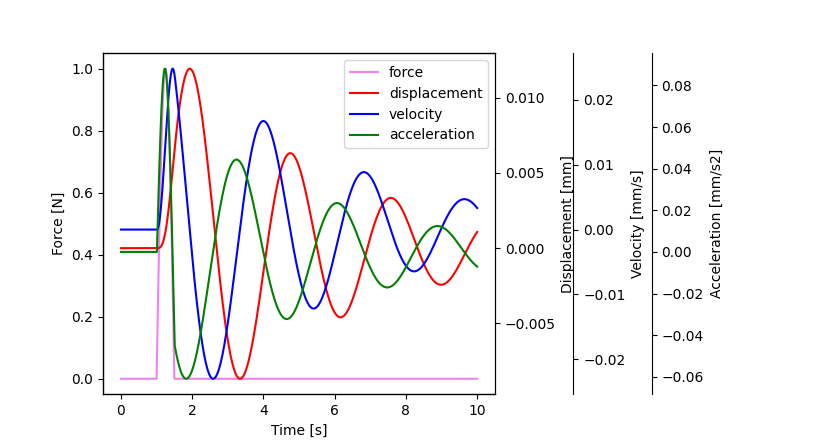
\includegraphics[width=0.90\textwidth]{img/euler_example.png}
    \caption{Euler's implementation for vibration problem example}
    \label{fig:euler-example-png}
\end{figure}


The \textbf{iterate()} function:
\begin{python}
def iterate(h, y0, func, rhs):
    num_of_odes = y0.shape[0]
    y1 = np.zeros(num_of_odes, dtype = float)
    for i in range(num_of_odes-1):
        y1[i] = y0[i] + y0[i+1] * h
    y1[-1] = func(y1, rhs)
    return y1

\end{python}

is written for general case of a set of ODEs. When considering the problem
of vibration (set of 2 ODEs):
\begin{python}
def iterate(h, u0, v0, a0, f, m , c, k):
    u1 = u0 + h * v0
    v1 = v0 + h * a0
    # m * a + c * v + k * u = f
    a1 = (f - c * v1 - k * u1) / m
    return np.array([u1, v1, a1], dtype=float)
\end{python}

which is the iteration of a set of \textbf{first order ODEs}:
\begin{eqarray}
    v &= \dot{u}\\
    \dot{v} &= \frac{f - c * v - k * u}{m}
\end{eqarray}


\newpage
\subsection{Runge-Kutta 4th order method}

\textbf{Runge-Kutta 4th order method} is another explicit method for solving
\textbf{first order ODEs}. The basic equation is:

\begin{equation}
    \frac{dy}{dx} = f(x,y) \quad , y(0) = y_0
\end{equation}

The formula for the next value $ y_{i+1} $ after a step size equal to $h $ is given by:

\begin{eqarray}
    k_1 &= h f(x_i, y_i)\\
    k_2 &= h f(x_i + \frac{h}{2}, y_i + \frac{k_1}{2})\\
    k_3 &= h f(x_i + \frac{h}{2}, y_i + \frac{k_2}{2})\\
    k_4 &= h f(x_i + h, y_i + k_3)\\
    y_{i+1} &= y_i + \frac{k_1}{6} + \frac{k_2}{3} + \frac{k_3}{3} + \frac{k_4}{6} + O(h^5)
\end{eqarray}

The formula basically computes next value $ y_{i+1} $ using current $ y_i $ plus
\textbf{weighted average of four increments}:

\begin{itemize}
    \item $ k_1 $ is the increment based on the slope at the beginning of the
    interval, using $ y $

    \item $ k_2 $ is the increment based on the slope at the midpoint of the interval,
        using $ y + h k_1 / 2 $

    \item $ k_3 $ is the increment based on the slope at the midpoint,
        using $ y + h k_2 / 2 $

    \item $ k_4 $ is the increment based on the slope at the end of the interval,
        using $ y + h k_3 / 2 $

\end{itemize}

The method is a fourth order method, meaning that the local truncation error is
on the order of $ O(h^5) $, while the total accumulated error is of order $ O(h^4) $.

\begin{figure}[ht]
    \centering
    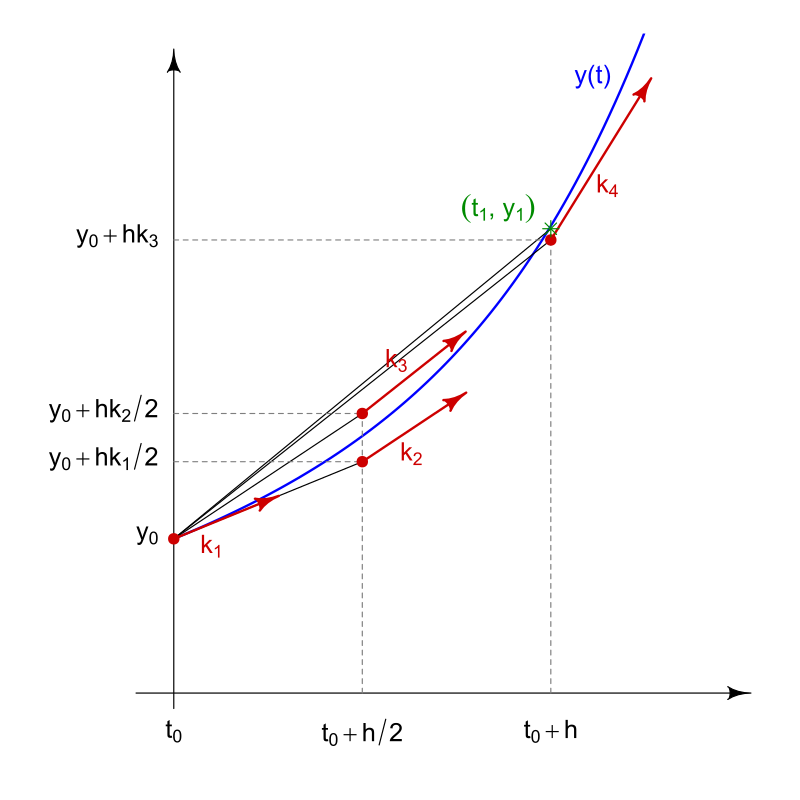
\includegraphics[width=0.80\textwidth]{img/Runge-Kutta_slopes.png}
    \caption{4th Order Runge-Kutta's method schematic}
    \label{fig:rk4-schema-png}
\end{figure}

\newpage
\begin{bbox}[0.96]
\textbf{Note:}

The formula for the next value $ y_{i+1} $ can be also written as:

\begin{eqarray}
    k_1 &= y_i\\
    k_2 &= y_i + \frac{h}{2} \frac{d k_1}{dx}\\
    k_3 &= y_i + \frac{h}{2} \frac{d k_2}{dx}\\
    k_4 &= y_i + h \frac{k_3}{dx}\\
    y_{i+1} &= y_i + \frac{h}{6} (\frac{d k_1}{dx} + 2 \frac{d k_2}{dx}
                              + 2 \frac{d k_3}{dx} + \frac{d k_4}{dx}) + O(h^5)
\end{eqarray}
\end{bbox}

\begin{bbox}[0.96]
This notation is more convenient to use when solving sets of ODEs for vibration
problem, because it translates to:

\begin{eqarray}
    u_1 &= u_0\\
    v_1 &= v_0\\
    a_1 &= (f - c v_0 - k u_0) / m\\
    u_2 &= u_0 + \frac{h}{2} v_1\\
    v_2 &= v_0 + \frac{h}{2} a_1\\
    a_2 &= (f - c v_1 - k u_1) / m\\
    u_3 &= u_0 + \frac{h}{2} v_2\\
    v_3 &= v_0 + \frac{h}{2} a_2\\
    a_3 &= (f - c v_2 - k u_2) / m\\
    u_4 &= u_0 + h v_3\\
    v_4 &= v_0 + h a_3\\
    a_4 &= (f - c v_3 - k u_3) / m\\
    u_{i+1} &= u_0 + \frac{h}{6} \left( v_1 + 2 v_2 + 2 v_3 + v_4 \right) \\
    v_{i+1} &= v_0 + \frac{h}{6} \left( a_1 + 2 a_2 + 2 a_3 + a_4 \right) \\
    a_{i+1} &= (f - c v_{i+1} - k u_{i+1}) / m\\
\end{eqarray}

where each of the \textbf{ODEs} are solved sequentially from the values
already known.

\end{bbox}

\newpage
\textbf{Python implementation for vibration problem:}

\begin{python}
#!/usr/bin/python3
import numpy as np
import matplotlib.pyplot as plt


def iterate(h, y0, y, func, rhs):
    num_of_odes = y0.shape[0]
    y1 = np.zeros(num_of_odes, dtype = float)
    for i in range(num_of_odes-1):
        y1[i] = y0[i] + y[i+1] * h
    y1[-1] = func(y1, rhs)
    return y1


def runge_kutta_4(t, y, func, rhs):
    N = t.shape[0]
    for j in range(N-1):
        dt = t[j+1] - t[j]
        y1 = iterate(0., y[j,:], y[j,:], func, rhs[j])
        y2 = iterate(dt/2, y[j,:], y1, func, 0.5 * (rhs[j+1] + rhs[j]))
        y3 = iterate(dt/2, y[j,:], y2, func, 0.5 * (rhs[j+1] + rhs[j]))
        y4 = iterate(dt, y[j,:], y3, func, rhs[j+1])

        # next step solution
        for i in range(y.shape[1]-1):
            y[j+1,i] = y[j,i] + dt/6 * (y1[i+1] + 2 * y2[i+1] + 2 * y3[i+1] + y4[i+1])
        y[j+1,-1] = func(y[j+1,:], rhs[j+1])
    return y


def rk4_vibration():
    m = 10.   # tonnes
    c = 5.    # Ns/mm
    k = 50.   # N/mm

    freq = np.sqrt(k / m) / (2 * np.pi)
    print(f'f = {freq}')

    # equation to solve
    # m * a + c * v + k * u = f
    # a = (f - c * v - k * u) / m
    acceleration = lambda u, f: (f - c * u[1] - k * u[0]) / m

    T = 10.     # seconds
    dt = 0.01   # timestep s
    u_0 = 0.    # mm of initial displacement
    v_0 = 0.    # mm/s of initial velocity

    # times at which to solve
    t = np.linspace(0, T, int(T/dt) + 1)

    # force vector
    F = 1.    # N of max impulse
    t0 = 1.   # impulse start time
    t1 = 1.5  # impuls end time
    f = np.zeros(t.shape[0], dtype=float)
    # create a half sine impulse of force
    for i in range(t.shape[0]):
        if t[i] >= t0 and t[i] <= t1:
            f[i] = F * np.sin((t[i] - t0) / (t1 - t0) * np.pi)
        else:
            f[i] = 0.

    uva = np.zeros((t.shape[0],3), dtype=float)
    uva[0,0] = u_0
    uva[0,1] = v_0

    uva = runge_kutta_4(t, uva, acceleration, f)

    fig, axf = plt.subplots()
    fig.subplots_adjust(right=0.60)

    p1, = axf.plot(t, f, label='force', color='violet')
    axu = axf.twinx()
    p2, = axu.plot(t, uva[:,0], label='displacement', color='red')
    axv = axf.twinx()
    axv.spines.right.set_position(('axes', 1.20))
    p3, = axv.plot(t, uva[:,1], label='velocity', color='blue')
    axa = axf.twinx()
    axa.spines.right.set_position(('axes', 1.40))
    p4, = axa.plot(t, uva[:,2], label='acceleration', color='green')

    axf.set_xlabel('Time [s]')
    axf.set_ylabel('Force [N]')
    axu.set_ylabel('Displacement [mm]')
    axv.set_ylabel('Velocity [mm/s]')
    axa.set_ylabel('Acceleration [mm/s2]')

    axf.legend(handles=[p1, p2, p3, p4])

    plt.show()

if __name__ == '__main__':
    rk4_vibration()

\end{python}

Which results to:
\begin{figure}[ht]
    \centering
    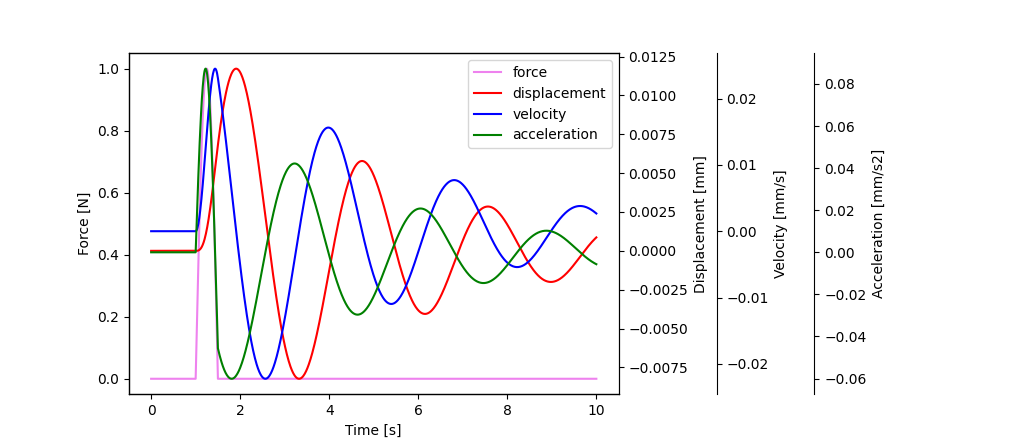
\includegraphics[width=0.90\textwidth]{img/rk4_example.png}
    \caption{4th order Runge-Kutta's implementation for vibration problem example}
    \label{fig:rk4-example-png}
\end{figure}



\newpage
\section{Implicit}

The basic approach is an incremental step-by-step solution with an assumtion
that the solution for a discrete time $ t $ is known and that the solution for
the discrete time $ t + \Delta t $ is required, where $ \Delta t $ is
a suitably chosen time increment. Hence, considering time $ t + \Delta t $:

\begin{equation}\label{implicit-equation}
    \m{F}^{t + \Delta t} - \m{N}^{t + \Delta t} = \m{0}
\end{equation}

Where $ \m{F} $ is the vector of external forces (loads) and $ \m{N} $
is the vector of inner forces.

Assume that $ \m{F}^{t + \Delta t} $ is independent of the deformations.
Since the solution is known at time $ t $, we can write:

\begin{equation}
    \m{N}^{t+\Delta t} = \m{N}^t + \Delta \m{N}
\end{equation}

where $ \Delta \m{N} $ is the increment in nodal point forces corresponding
to the increment in element displacements and stresses from time $ t $ to time
$ t + \Delta t $. This vector can be approximated using a \textbf{tangent stiffness matrix}
$ \m{K}^t $ which corresponds to the geometric and material conditions
at time $ t $,

\begin{equation}\label{internal-forces-approximation}
    \Delta \m{N} \doteq \m{K}^{t} \Delta \m{u}
\end{equation}

where $ \Delta \m{u} $ is a vector of incremental nodal point displacements and

\begin{equation}\label{tangent-stiffness-matrix}
    \m{K}^{t} = \frac{\partial \m{N}^{t}}{\partial \m{u}^{t}}
\end{equation}

Hence, the \textbf{tangent stiffness matrix} corresponds to the derivative of the
internal element nodal point forces $ \m{N}^{t} $ with respect to the
nodal point displacements $ \m{u}^{t} $.

Substituting \eqref{internal-forces-approximation} and
\eqref{tangent-stiffness-matrix} into \eqref{implicit-equation}, we obtain

\begin{equation}\label{iteration-equation}
    \m{K}^{t} \Delta \m{u} = \m{F}^{t + \Delta t} - \m{N}^{t}
\end{equation}

and solving for $ \m{u}^{\Delta t} $, we can calculate and approximation
to the displacements at time $ t + \Delta t $,

\begin{equation}\label{iteration-displacements}
    \m{u}^{t + \Delta t} \doteq \m{u}^{t} + \Delta \m{u}
\end{equation}

The exact displacements at time $ t + \Delta t $ are those that correspond to the
applied loads $ \m{F}^{t + \Delta t} $. We calculate in \eqref{iteration-displacements}
only an approximation to these displacements because \eqref{internal-forces-approximation}
was used.

Having evaluated an approximation to the displacements corresponding to
time $ t + \Delta t $, we could now solve for an approximation to the stresses and
corresponding nodal point forces at time $ t + \Delta t $, and then proceed to the
next time increment calculations. However, because of the assumption
\eqref{internal-forces-approximation}, such a solution may be subject to
very significant errors and, depending on the time or load step sizes used, may
indeed be unstable. In practice, it is therefore necessary to iterate until the
solution of \eqref{implicit-equation} is obtained to sufficient accuracy.


\subsection{Newton-Raphson}
Having calculated an \textit{increment} in nodal point displacements, which defones
a \textit{new total} displacement vector, we can repeat ht incremental solution
using the currently known total displacements at time $ t $.

The equations used in \textbf{Newton-Raphson} iteration are, $ for\ i = 1, 2, 3, \dots, $

\begin{bbox}
    \begin{eqarray}\label{newton-raphson}
        \m{K}_{i-1}^{t + \Delta t} \Delta \m{u}_i &=
        \m{F}^{t + \Delta t} - \m{N}_{i - 1}^{t + \Delta t} \\
        \m{u}_{i}^{t+\Delta t} &=  \m{u}_{i}^{t + \Delta t} +
        \m{u}_{i-1}^{t+\Delta t} + \Delta \m{u}_i
    \end{eqarray}
\end{bbox}

with the initial conditions:

\begin{eqarray}
    \m{u}_{0}^{t + \Delta t} &= \m{u}^t \\
    \m{K}_{0}^{t + \Delta t} &= \m{K}^t \\
    \m{N}_{0}^{t + \Delta t} &= \m{N}^t \\
\end{eqarray}

Note that in the first iteration, the relations in \eqref{newton-raphson}
reduce to the equations \eqref{iteration-equation} and \eqref{iteration-displacements}.
Then, in subsequent iterations, the latest estimates for the nodal point
displacements are used to evaluate the corresponding element stresses and
nodal point forces $ \m{N}_{i-1}^{t + \Delta t} $ and
\textbf{tangent stiffness matrix} $ \m{K}_{i-1}^{t + \Delta t} $.

The out-of-balance load vector $ \m{F}^{t + \Delta t} - \m{N}_{i-1}^{t + \Delta t} $
corresponds to a load vector that is not yet balanced by element stress, and
hence an increment in the nodal point displacement is required. This updating of the
nodal point displacement in the iteration is continued until out-of-balance loads
and incremental displacements are small enough.

An important point is that the calculation of $ \m{N}_{i-1}^{t + \Delta t} $
from $ \m{u}_{i-1}^{t + \Delta t} $ is \textbf{crucial}. Any errors in this
calculation will, in general, result in an incorrect response prediction.

The correct evaluation of the \textbf{tangent stiffness matrix}
$ \m{K}_{i-1}^{t + \Delta t} $ is also important. The use of proper
\textbf{tangent stiffness matrix} may be necessary for convergence and, in general,
will result in fewer iterations until convergence is reached.

However, because the expense involved in evaluating and factoring a new
\textbf{tangent stiffness matrix}, in practice, it can be more efficient,
depending on the nonlinearities present in the analysis, to evaluate a new
\textbf{tangent stiffness matrix} only at certain times. Specifically,
in the \textbf{modified Newton-Raphson method} a new \textbf{tangent stiffness matrix}
is established only at the beginning of each load step, and in
\textbf{quasi-Newton} methods \textbf{secant stiffness matrices} are used
instead of the tangent stiffness matrix.

The use of the iterative solution requires appropriate convergence criteria.
If inappropriate criteria are used, the iteration may be terminated before
the necessary solution accuracy is reached or be continued after the required
accuracy has been reached.

\subsubsection{Full Newton-Raphson Procedure derivation}

The finite element equilibrium requirements amount to finding the solution
of the equations:

\begin{equation}\label{nr-error}
    f( \m{u}^* ) = 0
\end{equation}

Where:

\begin{equation}\label{nr-error-expanded}
    f( \m{u}^* ) = \m{F}^{t + \Delta t} ( \m{u}^* )
    - \m{N}^{t + \Delta t} ( \m{u}^* )
\end{equation}

We denote here and in the following the complete array of the solution as
$ \m{u}^* $ but realize that this vector may also contain variables other
than displacements, for example, pressure variables and rotations.

Assume that in the iterative solution we have evaluated $ \m{u}_{i-1}^{t + \Delta t} $;
then a Taylor series expansion gives:

\begin{eqarray}\label{newton-raphson-taylor-expansion}
    f(\m{u}^*) &= f(\m{u}_{i-1}^{t + \Delta t})
    + \left. \left[\frac{\partial N}{\partial \m{u}} \right]
        \right|_{\m{u}_{i-1}^{t + \Delta t}}
        \left( \m{u}^* - \m{u}_{i-1}^{t + \Delta t} \right) \\
                    &+ higher\ order\ terms
\end{eqarray}

Substituting from \eqref{nr-error-expanded} into \eqref{newton-raphson-taylor-expansion}
and using \eqref{nr-error}, we obtain:

\begin{eqarray}\label{nr-taylor}
    & \left. \left[ \frac{\partial \m{N}}{\partial \m{u}} \right]
        \right|_{\m{u}_{i-1}^{t + \Delta t}}
    \left(\m{u}^* - \m{u}_{i-1}^{t + \Delta t} \right)
    + higher\ order\ terms\\
    & = \m{F}^{t + \Delta t} - \m{N}_{i-1}^{t + \Delta t}
\end{eqarray}

where we assumed that the externally applied loads are deformation independent.

Neglecting the higher-order terms in \eqref{nr-taylor}, we can calculate an increment
in the displacements,

\begin{equation}\label{nr-displacement-increment}
    \m{K}_{i-1}^{t + \Delta t} \Delta \m{u}_i =
    \m{F}^{t + \Delta t} - \m{N}_{i-1}^{t + \Delta t}
\end{equation}

where $ \m{K}_{i-1}^{t + \Delta t} $ is the current \textbf{tangent stiffness matrix}

\begin{equation}
     \m{K}_{i-1}^{t + \Delta t} =
     \left. \left[ \frac{\partial \m{N}}{\partial \m{u}} \right]
        \right|_{\m{u}_{i-1}^{t + \Delta t}}
\end{equation}

and the improved displacement solution is:

\begin{equation}\label{nr-displacement}
    \m{u}_i^{t + \Delta t} =
    \m{u}_{i-1}^{t + \Delta t} +
    \Delta \m{u}_{i}
\end{equation}

\textit{The relations in} \eqref{nr-displacement-increment} \textit{and} \eqref{nr-displacement}
\textit{costitute the Newton-Raphson solution of} \eqref{implicit-equation}.
Since an incremental analysis is performed with time (or load) steps of size
$ \Delta t $, the initial conditions in this iteration are
$ \m{K}_0^{t + \Delta t} = \m{K}^t $,
$ \m{N}_0^{t + \Delta t} = \m{N}^t $, and
$ \m{u}_0^{t + \Delta t} = \m{u}^t $.
The iteration is continued \textbf{until appropriate convergence criteria are satisfied.}

A characteristic of this iteration is that a new tangent stiffness matrix is
calculated in \textbf{each} iteration, which is why this method is also referred
to as the \textbf{full Newton-Raphson method}.

\begin{figure}[ht]
    \centering
    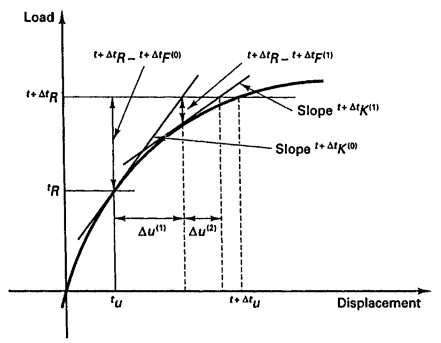
\includegraphics[width=0.60\textwidth]{img/full_newton_raphson.png}
    \caption{Newton-Raphson iteration in solution of SDOF system.
    $ \m{R} $ is load increment, $ \m{F} $ are internal forces,
    $ \m{u} $ are displacements.}
    \label{fig:full-newton-raphson-png}
\end{figure}



% TODO: Bathe FEP_2nd_Edidtion_4th_prinitng.pdf
%       Page 756 (773)
%       Modified Newton-Raphson




\newpage
\chapter{Model reduction}

\section{Guyan reduction}
\textbf{Guyan reduction}, also known as \textbf{static condensation},
is a \textit{dimensionality reduction} method which reduces the number
of \textbf{DOFs} by ignoring the interial terms of the equilibrium equations
and expressing the unloaded \textbf{DOFs} in terms of the loaded \textbf{DOFs}.

The static equilibrium equation:

\begin{eqarray}
    \begin{bmatrix}
        \m{K}_{mm} & \m{K}_{ms} \\
        \m{K}_{sm} & \m{K}_{ss}
    \end{bmatrix}
    \begin{bmatrix}
        \m{u}_m \\
        \m{u}_s
    \end{bmatrix} &=
    \begin{bmatrix}
        \m{f}_m \\
        \m{f}_s
    \end{bmatrix} \\
    \m{K}_{mm} \m{u}_m + \m{K}_{ms} \m{u}_s &= \m{f}_m \\
    \m{K}_{sm} \m{u}_m + \m{K}_{ss} \m{u}_s &= \m{f}_s
\end{eqarray}

Where $ m $ denotes the \textbf{master} DOFs and $ s $ the \textbf{slave} DOFs.
Stating that $ s $ section of the problem DOFs is unloaded, we can
write that $ \m{f}_s = \m{0} $. Then the slave DOFs are expressed
by the following equation:

\begin{equation}
    \m{K}_{sm} \m{u}_m + \m{K}_{ss} \m{u}_s = \m{0}
\end{equation}

Solving the above equation in terms of the independent (master) DOFs leads to
the following dependency relations:

\begin{equation}
    \m{u}_s = -\m{K}_{ss}^{-1} \m{K}_{sm} \m{u}_m
\end{equation}

Substituting the dependency relations to the upper (master) partition of the static
equilibrium problem condenses away the slave DOFs, leading to the following reduced
system of linear equations:

\begin{equation}
    \left(\m{K}_{mm} - \m{K}_{ms} \m{K}_{ss}^{-1} \m{K}_{sm} \right)
    \m{u}_m = \m{f}_m
\end{equation}

The above system of linear equations is equivalent to the original problem, but expressed
in terms of \textbf{master} DOFs alone. Thus, the \textbf{Guyan} reduction method
results in a reduced system by condensing away the \textbf{slave} DOFs.

The \textbf{Guyan reduction} can be also expressed as a \textit{change of basis} which
produces a low-dimensional representation of the original space, represented by the
\textbf{master} DOFs. The linear transformation that maps the reduced space onto
the full space is expressed as:

\begin{equation}
    \begin{bmatrix}
        \m{u}_m \\
        \m{u}_s
    \end{bmatrix} =
    \begin{bmatrix}
        \m{I} \\
        -\m{K}_{ss}^{-1} \m{K}_{sm}
    \end{bmatrix}
    \m{u}_m = \m{T}_G \m{u}_m
\end{equation}

where $ \m{T}_G $ represents the \textbf{Guyan} reduction \textit{transformation matrix}.
Thus, the reduced problem is represented as:

\begin{equation}
    \m{K}_G \m{u}_m = \m{f}_m
\end{equation}

In the above equation, $ \m{K}_G $ represents the reduced system of linear equations
that's obtained by applying the \textbf{Guyan reduction} transformation on the
full system, which is expressed as:

\begin{equation}
    \m{K}_G = \m{T}_G^T \m{K} \m{T}_G
\end{equation}

where $ \m{T}_G $ has the dimension of $ n_{DOF} \times n_m $.




\newpage
\chapter{Element Atlas}

\section{Matrices}

\textbf{The inversion formula for 3x3 matrix:}

\begin{eqarray}
    \m{A} &=
    \begin{bmatrix}
        a_{11} & a_{12} & a_{13}\\
        a_{21} & a_{22} & a_{23}\\
        a_{31} & a_{32} & a_{33}
    \end{bmatrix}\\
    \m{A}^{-1} &= \frac{1}{\vert \m{A} \vert}
    \begin{bmatrix}
        A_{11} & A_{12} & A_{13}\\
        A_{21} & A_{22} & A_{23}\\
        A_{31} & A_{32} & A_{33}
    \end{bmatrix}\\
\end{eqarray}

where:
\begin{eqarray}
    A_{11} &= a_{22} a_{33} - a_{23} a_{32}\\
    A_{22} &= a_{33} a_{11} - a_{31} a_{13}\\
    A_{33} &= a_{11} a_{22} - a_{12} a_{21}\\
    A_{12} &= a_{23} a_{31} - a_{21} a_{33}\\
    A_{23} &= a_{31} a_{12} - a_{32} a_{11}\\
    A_{31} &= a_{12} a_{23} - a_{13} a_{22}\\
    A_{21} &= a_{32} a_{13} - a_{12} a_{33}\\
    A_{32} &= a_{13} a_{21} - a_{23} a_{11}\\
    A_{13} &= a_{21} a_{22} - a_{31} a_{22}\\
    \vert A_{13} \vert &= a_{11} A_{11} + a_{12} A_{21} + a_{13} A_{31}
\end{eqarray}


\section{Numerical Integration}

\begin{bbox}
    \textbf{Note:}

    \textbf{Quadrature} is another term for \textbf{Numerical Integration}.
\end{bbox}


\subsection{Newton-Cotes quadrature}
In the most obvious procedure, points at which the function is to be formed are
determined \textit{a priori} - usually at equal intervals - and a polynomial
passed through the values of the function at these points and exactly integrated.

As $ n $ values define a polynomial of degree $ n - 1 $, the errors will be
of the order $ O(h^n) $ where $ h $ is the element size. This leads to the
well-known \textbf{Newton-Cotes} \'quadrature formulae\'. The integrals can be
written as:

\begin{equation}
    I = \int_{-1}^{1} f(\xi) d\xi = \sum_1^n H_i f(\xi_i)
\end{equation}

for the range of integration between $ -1 $ and $ +1 $. For example, if $ n = 2 $,
we have the well-known trapezoidal rule:

\begin{equation}
    I = f(-1) + f(1)
\end{equation}

for $ n = 3 $, the well-known \textbf{Simpson} one-third rule:

\begin{equation}
    I = \frac{1}{3} \left[ f(-1) + 4f(0) + f(1) \right]
\end{equation}

and for $ n = 4 $:

\begin{equation}
    I = \frac{1}{4} \left[f(-1) + 3f(-\frac{1}{3}) + 3f(\frac{1}{3}) + f(1) \right]
\end{equation}


\subsection{Gauss quadrature}

If in place of specifying the position of sampling points \textit{a priori} we
allow these to be located at points to be determined so as to aim for best
accuracy, then for a given number of sampling points increased accuracy can be
obtained. Indeed, if we again consider:

\begin{equation}
    I = \int_{-1}^{1} f(\xi) d\xi = \sum_1^n H_i f(\xi_i)
\end{equation}

and again assume a polynomial expression, it is easy to see that for $ n $ sampling
points we have $ 2n $ unknowns ($H_i$ and $\xi_i$) and hence a polynomial of degree
$ 2n-1 $ could be constructed and exactly integrated. The error is thus of order
$ O(h^{2n}) $.

The simultaneous equations involved are difficult to solve, but some mathematical
manipulation will show that the solution can be obtained explicitely in terms
of \textbf{Legendre polynomials}. Thus this particular process is frequently known
as \textbf{Gauss-Legendre} quadrature.

For purposes of finite elements analysis complex calculations are involved in
determining the values of $ f $, the function to be integratet. Thus the
Gauss-type processes, requiring the least number of such evaluations, are ideally
suited and are mostly used exvlusively.

Other expresssions for integration of functions of the type

\begin{equation}\label{leggaus}
    I = \int_{-1}^{1} w(\xi) f(\xi) d\xi = \sum_{1}^{n} H_i f(\xi_i)
\end{equation}

can be derived for prescribed forms of $ w(\xi) $, again integrating up to a certain
order of accuracy a polynomial expansion of $ f(\xi) $.


\subsection{Linear and Quadrilateral Elements}

\subsubsection{For 1D:}

\begin{equation}
    I = \int_{-1}^{1} f(\xi) d\xi = \sum_1^n H_i f(\xi_i)
\end{equation}


\subsubsection{For 2D:}

The most obvious way of obtaining the integral:

\begin{equation}
    I = \int_{-1}^{1} \int_{-1}^{1} f(\xi, \eta) d\xi d\eta
\end{equation}

Is to first evaluate the inner integral keeping $ \eta $ constant, i.e.:

\begin{equation}
    \int_{-1}^{1}f(\xi, \eta) d\xi = \sum_{j=1}^n H_j f(\xi_i, \eta) = \psi(\eta)
\end{equation}

Evaluating the outer integral in a similar manner, we have:

\begin{eqarray}
    I = \int_{-1}^{1} \psi(\eta) d\eta
    &= \sum_{i=1}^n H_i \psi(\eta_i)\\
    &= \sum_{i=1}^n H_i \sum_{j=1}^n H_j f(\xi_i,\eta_i)\\
    &= \sum_{i=1}^n \sum_{j=1}^n H_i H_j f(\xi_j,\eta_i)
\end{eqarray}

\subsubsection{For 3D:}
For a 3D element we have similarly:

\begin{eqarray}
    I &= \int_{-1}^{1} \int_{-1}^{1} \int_{-1}^{1} f(\xi, \eta, \mu) d\xi d\eta d\mu\\
    &= \sum_{i=1}^n \sum_{j=1}^n \sum_{k=1}^n H_i H_j f(\xi_i,\eta_j,\mu_k)
\end{eqarray}

In the above, the number of integrating points in each direction was assumed to be
the same. Clearly this is not necessary and on occasion it may be an advantage to
use different numbers in each direction of integration.

\begin{figure}[ht]
    \centering
    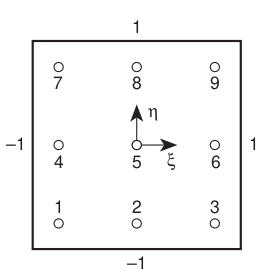
\includegraphics[width=0.25\textwidth]{img/quad_interpolation_3.png}
    \caption{Integration points for $ n = 3 $ in a square region. Exact for a
    polynomial of fifth order in each direction}
    \label{fig:quad-interpolation-3-png}
\end{figure}

\begin{table}
    \centering
    \renewcommand{\arraystretch}{1.25}
    \begin{tabular}{||c c c||}
        \hline
        \hline
        integration point & polynomial order & weight\\
        \hline
        \hline
        0 & n = 1 & 2.0\\
        \hline
        \begin{tabular}{c}
            $ -1/\sqrt{3} $ \\
            $ 1/\sqrt{3} $
        \end{tabular} & n = 2 &
        \begin{tabular}{c}
            1.0 \\
            1.0
        \end{tabular} \\
        \hline
        \begin{tabular}{c}
            $ -\sqrt{0.6} $ \\
            $ 0.0 $ \\
            $ \sqrt{0.6} $
        \end{tabular} & n = 3 &
        \begin{tabular}{c}
            $ 5/9 $ \\
            $ 8/9 $ \\
            $ 5/9 $
        \end{tabular} \\
        \hline
        \begin{tabular}{c}
            -0.861 136 311 594 953 \\
            -0.339 981 043 584 856 \\
             0.339 981 043 584 856 \\
             0.861 136 311 594 953 \\
        \end{tabular} & n = 4 &
        \begin{tabular}{c}
            0.347 854 845 137 454 \\
            0.652 145 154 862 546 \\
            0.652 145 154 862 546 \\
            0.347 854 845 137 454 \\
        \end{tabular} \\
        \hline
        \begin{tabular}{c}
            -0.906 179 845 938 664 \\
            -0.538 469 310 105 683 \\
             0.000 000 000 000 000 \\
             0.538 469 310 105 683 \\
             0.906 179 845 938 664 \\
        \end{tabular} & n = 5 &
        \begin{tabular}{c}
            0.236 926 885 056 189 \\
            0.478 628 670 499 366 \\
            0.568 888 888 888 889 \\
            0.478 628 670 499 366 \\
            0.236 926 885 056 189 \\
        \end{tabular} \\
        \hline
        \begin{tabular}{c}
            -0.932 469 514 203 152 \\
            -0.661 209 386 466 265 \\
            -0.238 619 186 083 197 \\
             0.238 619 186 083 197 \\
             0.661 209 386 466 265 \\
             0.932 469 514 203 152 \\
        \end{tabular} & n = 6 &
        \begin{tabular}{c}
            0.171 324 492 379 170 \\
            0.360 761 573 048 139 \\
            0.467 913 934 572 691 \\
            0.467 913 934 572 691 \\
            0.360 761 573 048 139 \\
            0.171 324 492 379 170 \\
        \end{tabular} \\
        \hline
        \begin{tabular}{c}
            -0.949 107 912 342 759 \\
            -0.741 531 185 599 394 \\
            -0.405 845 151 377 397 \\
             0.000 000 000 000 000 \\
             0.405 845 151 377 397 \\
             0.741 531 185 599 394 \\
             0.949 107 912 342 759 \\
        \end{tabular} & n = 7 &
        \begin{tabular}{c}
            0.129 484 966 168 870 \\
            0.279 705 391 489 277 \\
            0.381 830 050 505 119 \\
            0.471 959 183 673 469 \\
            0.381 830 050 505 119 \\
            0.279 705 391 489 277 \\
            0.129 484 966 168 870 \\
        \end{tabular} \\
        \hline
        \hline
    \end{tabular}
    \caption{Gauss-Legendre Integration Points and Weights}
\end{table}

\begin{bbox}
    To get the \textbf{Gauss-Legendre} points and weights in python use:

    \begin{python}
import numpy as np

# number of integration points
N = 3

points, weights = np.polynomial.legendre.leggauss(N)
    \end{python}
\end{bbox}


\newpage
\subsection{Triangular and Tetrahedral elements:}

\subsubsection{2D}
For a triangle, in terms of the \textbf{area coordinates} the integrals are of the
form:

\begin{equation}
    I = \int_{0}^{1} \int_{0}^{1-\xi} f(\xi, \eta, \mu) d\eta d\xi, \quad
    \mu = 1 - \xi - \eta
\end{equation}

Once again we could use $ n $ Gauss points and arrive at a summation expression of
the type used in the previous section. However, the limits of integration now
involve the variable itself and it is convenient to use alternative sampling points
for the second integration by use of a special Gauss expression for integrals of
the type given by equation \eqref{leggaus} in which $ w $ is a linear function.
These have been devised by \textit{Radau} and used successfully in finite element context.
It is, however, much more desirable (and aesthetically pleasing) to use special
formulae in which no bias is given to any of the natural coordinates ($\xi, \eta, \mu$).
Such formulae were first derived by \textit{Hammer et al.} and \textit{Felippa}
and a series of necessary sampling points and weights.

\newpage
\begin{table}[h!]
    \centering
    \renewcommand{\arraystretch}{1.25}
    % \small
    % \scriptsize
    \scalebox{0.80}{
    \begin{tabular}{||c c c c c c||}
        \hline
        \hline
        Order & Figure & Error & Points &
        \begin{tabular}{c} Triangular\\Coordinates\end{tabular} & Weights\\
        \hline
            Linear &
            \begin{tabular}{c}
                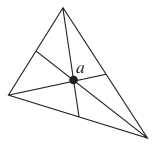
\includegraphics[width=0.20\textwidth]{img/tria_linear.png}\\
            \end{tabular}
            & $ R = O(h^2) $ & a & $ \frac{1}{3}, \frac{1}{3}, \frac{1}{3} $ & 1\\
        \hline
            Quadratic &
            \begin{tabular}{c}
                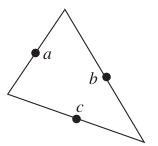
\includegraphics[width=0.20\textwidth]{img/tria_quadratic.png}
            \end{tabular}
            & $ R = O(h^3) $ & \begin{tabular}{c}
                a \\
                b \\
                c \\
            \end{tabular} & \begin{tabular}{c}
                $ \frac{1}{2}, \frac{1}{2} , 0 $ \\
                $ 0, \frac{1}{2}, \frac{1}{2} $ \\
                $ \frac{1}{2}, 0, \frac{1}{2} $ \\
            \end{tabular} & \begin{tabular}{c}
                $ \frac{1}{3} $ \\
                $ \frac{1}{3} $ \\
                $ \frac{1}{3} $ \\
            \end{tabular}\\
        \hline
            Cubic &
            \begin{tabular}{c}
                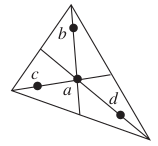
\includegraphics[width=0.20\textwidth]{img/tria_cubic.png}
            \end{tabular}
            & $ R = O(h^4) $ & \begin{tabular}{c}
                a \\
                b \\
                c \\
                d \\
            \end{tabular} & \begin{tabular}{c}
                $ \frac{1}{3}, \frac{1}{3} , \frac{1}{3} $ \\
                $ 0.6, 0.2, 0.2 $ \\
                $ 0.2, 0.6, 0.2 $ \\
                $ 0.2, 0.2, 0.6 $ \\
            \end{tabular} & \begin{tabular}{c}
                $ -\frac{27}{48} $ \\
                $ \frac{25}{48} $ \\
                $ \frac{25}{48} $ \\
                $ \frac{25}{48} $ \\
            \end{tabular}\\
        \hline
            Quintic &
            \begin{tabular}{c}
                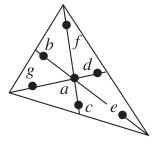
\includegraphics[width=0.20\textwidth]{img/tria_quintic.png}
            \end{tabular}
            & $ R = O(h^6) $ & \begin{tabular}{c}
                a \\
                b \\
                c \\
                d \\
                e \\
                f \\
                g \\
            \end{tabular} & \begin{tabular}{c}
                $ \frac{1}{3}, \frac{1}{3} , \frac{1}{3} $ \\
                $ \alpha_1, \beta_1, \beta_1 $ \\
                $ \beta_1, \alpha_1, \beta_1 $ \\
                $ \beta_1, \beta_1, \alpha_1 $ \\
                $ \alpha_2, \beta_2, \beta_2 $ \\
                $ \beta_2, \alpha_2, \beta_2 $ \\
                $ \beta_2, \beta_2, \alpha_2 $ \\
            \end{tabular} & \begin{tabular}{c}
                $ 0.225 000 000 0 $ \\
                $ 0.132 394 152 7 $ \\
                $ 0.132 394 152 7 $ \\
                $ 0.132 394 152 7 $ \\
                $ 0.125 939 180 5 $ \\
                $ 0.125 939 180 5 $ \\
                $ 0.125 939 180 5 $ \\
            \end{tabular}\\
            & & & \multicolumn{2}{l}{\begin{tabular}{l}
                with: \\
                $ \alpha_1 = $ 0.059 715 871 7 \\
                $ \beta_1 = $ 0.470 142 064 1 \\
                $ \alpha_2 = $ 0.797 426 985 3 \\
                $ \beta_2 = $ 0.101 286 507 3 \\
            \end{tabular}} & \\
        \hline
        \hline
    \end{tabular}}
    \caption{Triangular Element integration points and weights}
\end{table}


\newpage
\begin{table}[h!]
    \centering
    \renewcommand{\arraystretch}{1.25}
    % \small
    % \scriptsize
    \scalebox{0.80}{
    \begin{tabular}{||c c c c c c||}
        \hline
        \hline
        Order & Figure & Error & Points &
        \begin{tabular}{c} Tetrahedral\\Coordinates\end{tabular} & Weights\\
        \hline
            Linear &
            \begin{tabular}{c}
                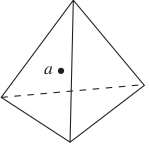
\includegraphics[width=0.20\textwidth]{img/tetra_linear.png}\\
            \end{tabular}
            & $ R = O(h^2) $ & a & $ \frac{1}{4}, \frac{1}{4}, \frac{1}{4}, \frac{1}{4} $ & 1\\
        \hline
            Quadratic &
            \begin{tabular}{c}
                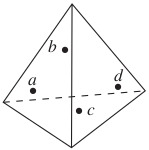
\includegraphics[width=0.20\textwidth]{img/tetra_quadratic.png}
            \end{tabular}
            & $ R = O(h^6) $ & \begin{tabular}{c}
                a \\
                b \\
                c \\
                d \\
            \end{tabular} & \begin{tabular}{c}
                $ \alpha, \beta, \beta, \beta $ \\
                $ \beta, \alpha, \beta, \beta $ \\
                $ \beta, \beta, \alpha, \beta $ \\
                $ \beta, \beta, \beta, \beta $ \\
            \end{tabular} & \begin{tabular}{c}
                $ \frac{1}{4} $ \\
                $ \frac{1}{4} $ \\
                $ \frac{1}{4} $ \\
                $ \frac{1}{4} $ \\
            \end{tabular}\\
            & & & \multicolumn{2}{l}{\begin{tabular}{l}
                with: \\
                $ \alpha = $ 0.585 410 20 \\
                $ \beta = $ 0.138 196 60 \\
            \end{tabular}} & \\
        \hline
            Cubic &
            \begin{tabular}{c}
                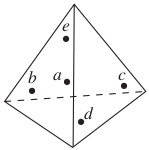
\includegraphics[width=0.20\textwidth]{img/tetra_cubic.png}
            \end{tabular}
            & $ R = O(h^4) $ & \begin{tabular}{c}
                a \\
                b \\
                c \\
                d \\
                e \\
            \end{tabular} & \begin{tabular}{c}
                $ \frac{1}{4}, \frac{1}{4}, \frac{1}{4}, \frac{1}{4} $ \\
                $ \frac{1}{2}, \frac{1}{6}, \frac{1}{6}, \frac{1}{6} $ \\
                $ \frac{1}{6}, \frac{1}{2}, \frac{1}{6}, \frac{1}{6} $ \\
                $ \frac{1}{6}, \frac{1}{6}, \frac{1}{2}, \frac{1}{6} $ \\
                $ \frac{1}{6}, \frac{1}{6}, \frac{1}{6}, \frac{1}{2} $ \\
            \end{tabular} & \begin{tabular}{c}
                $ -\frac{4}{5} $ \\
                $ \frac{9}{20} $ \\
                $ \frac{9}{20} $ \\
                $ \frac{9}{20} $ \\
                $ \frac{9}{20} $ \\
            \end{tabular}\\
        \hline
        \hline
    \end{tabular}}
    \caption{Tetrahedral Element integration points and weights}
\end{table}



\newpage
\section{General Element Matrices Procedure}
The procedure to generate any element stiffness, mass and load matrices can
be generalised to the following steps:

\begin{enumerate}
    \item Create Element domain in natural coordinates:
        \begin{itemize}
            \item $ -1 $ to $ 1 $ for quadrilateral elements
            \item $ 0 $ to $ 1 $ for triangular and linear elements
        \end{itemize}

    \item select the number of Gauss points based on the order of the element
        \begin{itemize}
            \item $ 2 $ for linear elements
            \item $ 3 $ for quadratic elements
        \end{itemize}

        Example:
        \begin{python}
import numpy as np
gp, gw = np.polynomial.legendre.leggauss(3)
        \end{python}

    \item Generate the shape functions $ \m{N}_n^e $ in natural coordinates
        based on the number of Gauss points, dimension of the element and its domain.

        The $ \m{N}_n^e $ matrix has the dimensions of:
        \begin{itemize}
            \item number of integration points = number of rows
            \item number of shape functions = number of columns
        \end{itemize}

        Therefore:

        \begin{equation}
            \m{N}_n^e = \begin{bmatrix}
                N_{1,1}^e & \dots & N_{n,1}^e\\
                \vdots & \vdots & \vdots\\
                N_{1,m}^e & \dots & N_{n,m}^e
            \end{bmatrix}
        \end{equation}
         where $ 1 \dots m $ are the integration points and $ 1 \dots n $ are the shape
         functions.

    \item Transform the shape functions from natural coordinates to global coordinates
        \begin{eqarray}
            \m{N}_g^e &= \m{N}_n^e \m{x}^e\\
            \m{N}_g^e &= \begin{bmatrix}
                N_{1,1}^e(\xi) & \dots & N_{n,1}^e(\xi)\\
                \vdots & \vdots & \vdots\\
                N_{1,m}^e(\xi) & \dots & N_{n,m}^e(\xi)
            \end{bmatrix}
            \begin{bmatrix}
                x_1 & y_1 & z_1\\
                \vdots & \vdots & \vdots\\
                x_n & y_n & z_n
            \end{bmatrix}
        \end{eqarray}

        The $ \m{x}^e $ matrix is a matrix of global coordinates of the element nodes.

        The resulting matrix has the dimension of:
        \begin{itemize}
            \item number of integration points = number of rows
            \item number of coordinates = number of columns (3D = 3, 2D = 2)
        \end{itemize}

    \item Generate the shape functions derivatives $ \m{B}_n^e $
        in natural coordinates

        The shape functions derivatives matrix has 3 dimensions being
        \textit{number of integration points} $\times$ \textit{number of natural coordinates}
        $\times$ \textit{number of shape functions}

    \item Create the Matrix of Jacobians from the shape functions derivatives:
        \begin{equation}
            \m{J} = \m{B}_n^e \m{x}^e
        \end{equation}

        The Matrix of Jacobians has the dimension of \textit{number of integration points}
        $\times$ \textit{number of global coordinates}
        $\times$ \textit{number of global coordinates}, where number of global coordinates
        means 2 for 2D and 3 for 3D problem.

    \item Get the Matrix of Jacobian determinants and an inverse Jacobian:
        \begin{equation}
            \m{J}^{-1}\\
            \m{J}_d = det \m{J}
        \end{equation}

        Example:
        \begin{python}
d_jacobi = np.linalg.det(jacobi)
i_jacobi = np.linalg.inv(jacobi)
        \end{python}

        The Jacobian determinant is computed for each integration point and has a dimension
        of \textit{number of integration points} $\times$ \textit{1}

        The inverse Jacobian has the same dimension as the Jacobian (\textbf{must have})

    \item Transform the shape function derviatives from natural coordinates to
        global coordinates
        \begin{equation}
            \m{B}_g^e = \m{J}^{-1} \m{B}_n^e
        \end{equation}

    \item Create the Material Stiffness matrix $ \m{C} $

    \item Finally for each integration point:

        3D:
        \begin{eqarray}
            \m{B}_{i,x}^e &= \m{B}_g(i, 0) \\
            \m{B}_{i,y}^e &= \m{B}_g(i, 1) \\
            \m{B}_{i,z}^e &= \m{B}_g(i, 2)\\
        \end{eqarray}

        where $ \m{B}_{i,x}^e $,  $ \m{B}_{i,y}^e $ and  $ \m{B}_{i,z}^e $
        are vectors of legth = \textit{number of shape functions}

        Then matrix $ \m{B} $ is:

        \begin{equation}
            \m{B}_i = \begin{bmatrix}
                \m{B}_{i,x}^e & \m{0} & \m{0}\\
                \m{0} & \m{B}_{i,y}^e & \m{0}\\
                \m{0} & \m{0} & \m{B}_{i,z}^e \\
                \m{B}_{i,y}^e & \m{B}_{i,x}^e & \m{0}\\
                \m{0} & \m{B}_{i,z}^e & \m{B}_{i,y}^e \\
                \m{B}_{i,z}^e & \m{0} & \m{B}_{i,x}^e
            \end{bmatrix}
        \end{equation}

        and matrix $ \m{N} $ is:

        \begin{equation}
            \m{N}_i = \begin{bmatrix}
                \m{N}_{n,i}^e & \m{0} & \m{0}\\
                \m{0} & \m{N}_{n,i}^e & \m{0}\\
                \m{0} & \m{0} & \m{N}_{n,i}^e
            \end{bmatrix}
        \end{equation}

        where $ \m{0} $ is a zero vector of length = \textit{number of shape functions}
        and $ \m{N}_{n,i}^e $ is a vector of shape functions in natural coordinates
        pertaining to the $i$-th integration point.

        Then:

        \begin{enumerate}
            \item \begin{equation}
                    \m{K}_i^e = \m{B}_i^T \m{C} \m{B}_i \ det \m{J}_i
                    w_i
                  \end{equation}

            \item \begin{equation}
                    \m{M}_i^e = \rho \m{N}_i^T \m{N}_i \ det \m{J}_i
                    w_i
                  \end{equation}
            \item \begin{equation}
                    \m{F}_i^e = \m{N}_i^T \m{F} \ det \m{J}_i
                    w_i
                  \end{equation}

                  where $ \m{F} = \begin{bmatrix}f_x \\ f_y \\ f_z\end{bmatrix} $
        \end{enumerate}

        where $ w_i $ is the multiple of gaussian weights for the respective
        integration point (for 3D case brick where the natural coordinates
        are $ \xi $, $ \eta $, $ \mu $ the $ w_i = w_{\xi_i} w_{\eta_i} w_{\mu_i} $

    \item Finally:
        \begin{enumerate}
            \item \begin{equation}
                    \m{K}^e = \sum_{i=1}^n \m{K}_i^e
                \end{equation}

            \item \begin{equation}
                    \m{M}^e = \sum_{i=1}^n \m{M}_i^e
                \end{equation}

            \item \begin{equation}
                    \m{F}^e = \sum_{i=1}^n \m{F}_i^e
                \end{equation}
        \end{enumerate}
\end{enumerate}


\newpage
\section{ROD}

\subsection{Element Formulation}
The \textbf{rod} element is a 1-D linear element. It has 2 nodes, and 3 dofs for
each node $ u_x, u_y, u_y $ (or $ u, v, w $). Rotation \textbf{DOF}s are not
constrained.

\subsubsection{Natural coordinates}
The natural coordinate $ \xi $ of the \textbf{ROD} element goes from $ 0 $ to $ 1 $.
The 2-noded rod element is defined by:

\begin{equation}
    \begin{bmatrix}
        1 \\
        x \\
        y \\
        z \\
        u_x \\
        u_y \\
        u_z \\
    \end{bmatrix}
    = \begin{bmatrix}
        1 & 1 \\
        x_1 & x_2 \\
        y_1 & y_2 \\
        z_1 & z_2 \\
        u_{x1} & u_{x2} \\
        u_{y1} & u_{y2} \\
        u_{z1} & u_{z2} \\
    \end{bmatrix}
    \begin{bmatrix}
        N_1^e \\
        N_2^e \\
    \end{bmatrix}
\end{equation}

\subsubsection{Shape Functions}
The \textbf{ROD} natural coordinates are:

\begin{table}[ht]
    \centering
    \begin{tabular}{|c c |}
        \hline
        node & $\xi$ \\
        \hline
        1 & 0 \\
        2 & 1 \\
        \hline
    \end{tabular}\\
    \caption{ROD corners natural coordinates}
\end{table}

The shape functions are:

\begin{eqarray}
    N_1^e &= 1 - \xi \\
    N_2^e &= \xi \\
\end{eqarray}


\subsubsection{Partial Derivatives}
The shape function derivatives with respect to the natural coordinate:

\begin{eqarray}
    \frac{\partial N_1^e}{\partial \xi} &= -1 \\
    \frac{\partial N_2^e}{\partial \xi} &= \phantom{-}1 \\
\end{eqarray}

\subsubsection{The Jacobian}

The derivatives of the shape functions are given by the usual chain rule formula:
\begin{eqarray}
    \frac{\partial N_i^e}{\partial x} &= \frac{\partial N_i^e}{\partial \xi}
                                         \frac{\partial \xi}{\partial x} \\
    \frac{\partial N_i^e}{\partial y} &= \frac{\partial N_i^e}{\partial \xi}
                                         \frac{\partial \xi}{\partial y} \\
    \frac{\partial N_i^e}{\partial z} &= \frac{\partial N_i^e}{\partial \xi}
                                         \frac{\partial \xi}{\partial z} \\
\end{eqarray}

In matrix form:
\begin{equation}
    \begin{bmatrix}
        \frac{\partial N_i^e}{\partial x} \\
        \frac{\partial N_i^e}{\partial y} \\
        \frac{\partial N_i^e}{\partial z} \\
    \end{bmatrix}
    = \begin{bmatrix}
        \frac{\partial \xi}{\partial x} \\
        \frac{\partial \xi}{\partial y} \\
        \frac{\partial \xi}{\partial z} \\
    \end{bmatrix}
    \begin{bmatrix}
        \frac{\partial N_i^e}{\partial \xi} \\
    \end{bmatrix}
\end{equation}

The $ 3 \times 1 $ matrix above is $ \m{J}^{-1} $, the inverse of:
\begin{equation}
    \m{J} = \frac{\partial (x, y, z)}{\partial(\xi)} =
    \begin{bmatrix}
        \frac{\partial x}{\partial \xi} &
        \frac{\partial y}{\partial \xi} &
        \frac{\partial z}{\partial \xi} \\
    \end{bmatrix}
\end{equation}

Given the element coordinates the Jacobian can be computed:
\begin{equation}
    \m{J}_i = \begin{bmatrix}
        \frac{\partial N_i^e}{\partial \xi} &
        \frac{\partial N_i^e}{\partial \xi} &
        \frac{\partial N_i^e}{\partial \xi} \\
    \end{bmatrix}
    \begin{bmatrix}
        x_i \\
        y_i \\
        z_i \\
    \end{bmatrix}
\end{equation}

end then numerically inverted for $ \m{J}^{-1} $.

\begin{bbox}
    If the $ \m{J} $ is not a square matrix, then \textbf{Moore-Penrose pseudoinverse}
    applies:

    \begin{equation}
        \m{J}^{-1} = \m{J}^{+} = \left( \m{J}^T \m{J} \right)^{-1} \m{J}^T
    \end{equation}

    in python:

    \begin{minted}[linenos=true, xleftmargin=1cm]{python}
        import numpy as np

        J_i = np.linalg.pinv(J)
    \end{minted}

\end{bbox}

\begin{bbox}
    Assembling the \textbf{Jacobian} thegether gives essentially that for a 1D case

    \begin{equation}
        \m{J} = l
    \end{equation}

    and therefore:
    \begin{equation}
        \m{J}^{-1} = \frac{1}{l}
    \end{equation}

    \begin{equation}
        \det{J} = l
    \end{equation}
\end{bbox}

afterwards for each integration point:
\begin{equation}
    \m{N}^i_g = \m{N}^i \m{u}
\end{equation}

\begin{equation}
    \m{B}^i_g = {\m{J}^i}^{-1} \frac{\partial N}{\partial \xi}^i
\end{equation}

then:
\begin{eqarray}
    \m{K}^e &\eqp {\m{B}^i_g}^T \m{D} {\m{B}^i_g} \det \m{J}^i w^i \\
    \m{M}^e &\eqp \rho {\m{N}^i}^T {\m{N}^i} \det \m{J}^i w^i \\
    \m{F}^e &\eqp {\m{N}^i}^T \m{F} \det \m{J}^i w^i \\
\end{eqarray}





\subsection{Example 1D}
If assembling the element in local CSYS, then $ u_y = 0 $ and $ u_z = 0 $.
Simplifiying the equations gives that:
\begin{equation}
    \m{N} = \begin{bmatrix}
        N_1^e & N_2^e \\
    \end{bmatrix}
    = \begin{bmatrix}
        1 - \xi & \xi \\
    \end{bmatrix}
\end{equation}

and
\begin{equation}
    u^e(\xi) = \m{N} \begin{bmatrix}
        u_1^e \\
        u_2^e \\
    \end{bmatrix}
\end{equation}

shape function derivatives:
\begin{equation}
    \m{B} = \frac{\partial \m{N}}{\partial \xi} =
    \begin{bmatrix}
        -1 & 1 \\
    \end{bmatrix}
\end{equation}

the strain-displacement realtion is given by:
\begin{equation}
    \M{\epsilon} = \m{B} \m{u}
\end{equation}

Integrating the element at midpoint $ \xi = 0.5 $ with a weight of $ w = 1.0 $
(for interval $ \left< 0, 1 \right> $, for an interval
$ \left< -1,  1 \right> $ the weight is $ w = 2.0 $)

\begin{equation}
    \m{N} = \begin{bmatrix}
        0.5 & 0.5 \\
    \end{bmatrix}
\end{equation}

Shape Functions in global coordinates:

\begin{equation}
    \m{N} = 0.5 u_1 + 0.5 u_2 = 0.5 (u_1 + u_2)
\end{equation}

Shape Function Derivatives in Natural Coordinates:

\begin{equation}
    \m{B} = \begin{bmatrix}
        -1 & 1 \\
    \end{bmatrix}
\end{equation}

Jacobian:

\begin{equation}
    \m{J} = \m{B} \m{u} = \begin{bmatrix}
        -1 & 1 \\
    \end{bmatrix}
    \begin{bmatrix}
        u_1 \\
        u_2 \\
    \end{bmatrix}
    = u_2 - u_1 = l
\end{equation}

Jacobian Determinant:

\begin{equation}
    \det \m{J} = l
\end{equation}

Jacobian Inverse:

\begin{equation}
    \m{J}^{-1} = \frac{1}{l}
\end{equation}

Shape function derivatives in global coordinates:

\begin{equation}
    \m{B}_g = \m{J}^{-1} \m{B} = \frac{1}{l}
    \begin{bmatrix}
        -1 & 1 \\
    \end{bmatrix}
\end{equation}

Material Stiffness Matrix

\begin{equation}
    \m{D} = EA
\end{equation}

Then for each integration point (here $1$):

\begin{eqarray}
    \m{K}^e &\eqp \m{B}_g^T \m{D} \m{B_g} \det \m{J} w \\
    \m{K}^e &\eqp \frac{1}{l} \begin{bmatrix} -1 \\ 1 \\ \end{bmatrix}
                  EA
                  \frac{1}{l} \begin{bmatrix} -1 & 1 \\ \end{bmatrix}
                  l 1 \\
    \m{K}^e &\eqp \frac{EA}{l}
                  \begin{bmatrix} -1 \\ 1 \\ \end{bmatrix}
                  \begin{bmatrix} -1 & 1 \\ \end{bmatrix} \\
    \m{K}^e &\eqp \frac{EA}{l}
                  \begin{bmatrix}
                      \phantom{-}1 & -1 \\
                      -1 & \phantom{-}1 \\
                  \end{bmatrix}
\end{eqarray}


\subsection{Example 2D}
If assembling the element in 2D, then and $ u_z = 0 $.
Simplifiying the equations gives that:
\begin{equation}
    \m{N} = \begin{bmatrix}
        N_1^e & 0 & N_2^e & 0 \\
        0 & N_1^e & 0 & N_2^e \\
    \end{bmatrix}
    = \begin{bmatrix}
        1 - \xi & 0 & \xi & 0 \\
        0 & 1 - \xi & 0 & \xi \\
    \end{bmatrix}
\end{equation}

and
\begin{equation}
    \begin{bmatrix}
        u_x^e(\xi) \\
        u_y^e(\xi) \\
    \end{bmatrix}
    = \m{N} \begin{bmatrix}
        u_{x1}^e \\
        u_{y1}^e \\
        u_{x2}^e \\
        u_{y2}^e \\
    \end{bmatrix}
\end{equation}

or if:
\begin{equation}
    \m{N} = \begin{bmatrix}
        N_1^e & N_2^e \\
    \end{bmatrix}
    = \begin{bmatrix}
        1 - \xi & \xi \\
    \end{bmatrix}
\end{equation}

then:
\begin{equation}
    \begin{bmatrix}
        u_x^e(\xi) \\
        u_y^e(\xi) \\
    \end{bmatrix}
    = \m{N} \begin{bmatrix}
        u_{x1}^e & u_{y1}^e \\
        u_{x2}^e & u_{y2}^e \\
    \end{bmatrix}
\end{equation}

shape function derivatives:
\begin{equation}
    \m{B} = \frac{\partial \m{N}}{\partial \xi} =
    \begin{bmatrix}
        -1 & \phantom{-}0 & 1 & 0 \\
        \phantom{-}0 & -1 & 0 & 1  \\
    \end{bmatrix}
\end{equation}

the strain-displacement realtion is given by:
\begin{equation}
    \M{\epsilon} = \m{B} \m{u}
\end{equation}

Integrating the element at midpoint $ \xi = 0.5 $ with a weight of $ w = 1.0 $
(for interval $ \left< 0, 1 \right> $, for an interval
$ \left< -1,  1 \right> $ the weight $ w = 2.0 $)
then numerically:

\begin{equation}
    \m{N} = \begin{bmatrix}
        0.5 & 0.5 \\
    \end{bmatrix}
\end{equation}

Shape Functions in global coordinates:

\begin{equation}
    \m{N} = \begin{bmatrix}
        1 - \xi & 0 & \xi & 0 \\
        0 & 1 - \xi & 0 & \xi \\
    \end{bmatrix}_{\xi = 0.5}
    \begin{bmatrix}
        u_{x1}^e \\
        u_{y1}^e \\
        u_{x2}^e \\
        u_{y2}^e \\
    \end{bmatrix}
    = \begin{bmatrix}
        0.5 u_{x1} + 0.5 u_{x2} \\
        0.5 u_{y1} + 0.5 u_{y2} \\
    \end{bmatrix}
\end{equation}

Shape Function Derivatives in Natural Coordinates (there is a row for each
integration point if the coordinates are specified as matrix, not a column
vector. otherwise for each integration point there is a separate $ \m{B} $
matrix):

\begin{equation}
    \frac{\partial \m{N}}{\partial \xi} =
    \m{B} = \begin{bmatrix}
        -1 & 0 & 1 & 0 \\
        0 & -1 & 0 & 1 \\
    \end{bmatrix}
\end{equation}

Jacobian:

\begin{equation}
    \m{J} = \m{B} \m{u} =
    \begin{bmatrix}
        -1 & \phantom{-}0 & 1 & 0 \\
        \phantom{-}0 & -1 & 0 & 1  \\
    \end{bmatrix}
    \begin{bmatrix}
        u_{x1}^e \\
        u_{y1}^e \\
        u_{x2}^e \\
        u_{y2}^e \\
    \end{bmatrix}
    = \begin{bmatrix}
        u_{x2}^e - u_{x1}^e \\
        u_{y2}^e - u_{y1}^e \\
    \end{bmatrix}
    = \begin{bmatrix}
        l_x \\
        l_y \\
    \end{bmatrix}
\end{equation}

\begin{qbox}

    Jacobian Determinant (when the \textbf{Jacobian matrix} is a vector, its
    determinant is simply its \textbf{length}):

\end{qbox}

\begin{equation}
    \det \m{J} = || \m{J} || = \sqrt{J_1^2 + J_2^2} = \sqrt{l_x^2 + l_y^2} = l
\end{equation}


\begin{qbox}

    Jacobian Inverse (when the \textbf{Jacobian matrix} is a row vector, its inverse
    is just its \textbf{transpose} divided by its determinant squared):

    \textbf{Moore-Penrose pseudoinverse}:
    \begin{eqarray}
        \boxed{\m{J}^{-1}} =
        \m{J}^{+} &= \left( \m{J}^T \m{J} \right)^{-1} \m{J}^T \\
                  &= \left(
                      \begin{bmatrix}
                          l_x & l_y \\
                      \end{bmatrix}
                      \begin{bmatrix}
                          l_x \\
                          l_y \\
                      \end{bmatrix}
                  \right)^{-1}
                      \begin{bmatrix}
                          l_x & l_y \\
                      \end{bmatrix} \\
                  &= \left( l_x^2 + l_y^2 \right)^{-1}
                      \begin{bmatrix}
                          l_x & l_y \\
                      \end{bmatrix} \\
                  &= \frac{1}{l_x^2 + l_y^2}
                      \begin{bmatrix}
                          l_x & l_y \\
                      \end{bmatrix} \\
                  &= \frac{1}{\sqrt{l_x^2 + l_y^2}^2}
                      \begin{bmatrix}
                          l_x & l_y \\
                      \end{bmatrix} \\
                  &= \boxed{\frac{1}{l^2} \m{J}^T}
    \end{eqarray}

\end{qbox}

\begin{equation}
    \m{J}^{-1} = \frac{1}{l^2}
    \begin{bmatrix}
        l_x & l_y \\
    \end{bmatrix}
    = \frac{1}{l}
    \begin{bmatrix}
        c & s \\
    \end{bmatrix}
\end{equation}

where $ c = \cos \varphi = l_x / l $ and $ s = \sin \varphi = l_y / l $.

Shape function derivatives in global coordinates:

\begin{equation}
    \m{B}_g
    = \m{J}^{-1} \m{B}
    = \frac{1}{l}
    \begin{bmatrix}
        c & s \\
    \end{bmatrix}
    \begin{bmatrix}
        -1 & \phantom{-}0 & 1 & 0 \\
        \phantom{-}0 & -1 & 0 & 1  \\
    \end{bmatrix}
    = \frac{1}{l}
    \begin{bmatrix}
        -c & -s & c & s
    \end{bmatrix}
\end{equation}

Material Stiffness Matrix

\begin{equation}
    \m{D} = EA
\end{equation}

Then for each integration point (here $1$):

\begin{equation}
    \m{K}^e \eqp \m{B}_g^T \m{D} \m{B_g} \det \m{J} w
\end{equation}

\begin{eqarray}
    \m{K}^e &\eqp
    \frac{1}{l}
    \begin{bmatrix}
        -c \\
        -s \\
        \phantom{-}c \\
        \phantom{-}s \\
    \end{bmatrix}
    EA
    \frac{1}{l}
    \begin{bmatrix}
        -c & -s & c & s
    \end{bmatrix}
    l w \\
    &\eqp
    \frac{EA}{l}
    \begin{bmatrix}
        c^2 & c s & -c^2 & -cs \\
        cs & s^2 & -cs & -s^2 \\
        -c^2 & -c s & c^2 & cs \\
        -cs & -s^2 & cs & s^2 \\
    \end{bmatrix} w
\end{eqarray}

which is the same result as when the element stiffness matrix is derived
in local coordinate system for a situation where $ \xi $ axis coincides with
the element $ x $ axis and the $ u_y $ component is $ 0 $. Afterwards,
the element \textbf{stiffness} and \textbf{mass} matrices as well as
\textbf{forces} vector are tranformed to the global CSYS using a transformation
matrix $ \m{T} $:

\begin{equation}
    \m{K}_l^e = \frac{EA}{l}
    \begin{bmatrix}
        \phantom{-}1 & 0 & -1 & 0 \\
        \phantom{-}0 & 0 & \phantom{-}0 & 0 \\
        -1 & 0 & \phantom{-}1 & 0 \\
        \phantom{-}0 & 0 & \phantom{-}0 & 0 \\
    \end{bmatrix}
\end{equation}

\begin{equation}
    \m{T} = \begin{bmatrix}
        \phantom{-}c & s & \phantom{-}0 & 0 \\
        -s & c & \phantom{-}0 & 0 \\
        \phantom{-}0 & 0 & \phantom{-}c & s \\
        \phantom{-}0 & 0 & -s & c \\
    \end{bmatrix}
\end{equation}

then the global element stiffness matrix is defined:

\begin{eqarray}
    \m{K}_g^e &= \m{T}^T \m{K}_l^e \m{T} \\
    &= \frac{EA}{l}
    \begin{bmatrix}
        c & -s & 0 & \phantom{-}0 \\
        s & \phantom{-}c & 0 & \phantom{-}0 \\
        0 & \phantom{-}0 & c & -s \\
        0 & \phantom{-}0 & s & \phantom{-}c \\
    \end{bmatrix}
    \begin{bmatrix}
        \phantom{-}1 & 0 & -1 & 0 \\
        \phantom{-}0 & 0 & \phantom{-}0 & 0 \\
        -1 & 0 & \phantom{-}1 & 0 \\
        \phantom{-}0 & 0 & \phantom{-}0 & 0 \\
    \end{bmatrix}
    \begin{bmatrix}
        \phantom{-}c & s & \phantom{-}0 & 0 \\
        -s & c & \phantom{-}0 & 0 \\
        \phantom{-}0 & 0 & \phantom{-}c & s \\
        \phantom{-}0 & 0 & -s & c \\
    \end{bmatrix} \\
    &= \frac{EA}{l}
    \begin{bmatrix}
        c & -s & 0 & \phantom{-}0 \\
        s & \phantom{-}c & 0 & \phantom{-}0 \\
        0 & \phantom{-}0 & c & -s \\
        0 & \phantom{-}0 & s & \phantom{-}c \\
    \end{bmatrix}
    \begin{bmatrix}
        c & s & -c & -s \\
        0 & 0 & 0 & 0 \\
        -c & -s & c & s \\
        0 & 0 & 0 & 0 \\
    \end{bmatrix} \\
    &= \frac{EA}{l}
    \begin{bmatrix}
        c^2 & cs & -c^2 & -cs \\
        cs & s^2 & -cs & -s^2 \\
        -c^2 & -cs & c^2 & cs \\
        -cs & -s^2 & cs & s^2 \\
    \end{bmatrix}
\end{eqarray}





\subsection{Example 3D}
If assembling the element in 3D, then and $ u_z \neq 0 $.
Simplifiying the equations gives that:
\begin{equation}
    \m{N} = \begin{bmatrix}
        N_1^e & 0 & 0 & N_2^e & 0 & 0 \\
        0 & N_1^e & 0 & 0 & N_2^e & 0 \\
        0 & 0 & N_1^e & 0 & 0 & N_2^e \\
    \end{bmatrix}
    = \begin{bmatrix}
        1 - \xi & 0 & 0 & \xi & 0 & 0 \\
        0 & 1 - \xi & 0 & 0 & \xi & 0  \\
        0 & 0 & 1 - \xi & 0 & 0 & \xi \\
    \end{bmatrix}
\end{equation}

and
\begin{equation}
    \begin{bmatrix}
        u_x^e(\xi) \\
        u_y^e(\xi) \\
        u_z^e(\xi) \\
    \end{bmatrix}
    = \m{N}(\xi) \begin{bmatrix}
        u_{x1}^e \\
        u_{y1}^e \\
        u_{z1}^e \\
        u_{x2}^e \\
        u_{y2}^e \\
        u_{z2}^e \\
    \end{bmatrix}
\end{equation}

or if:
\begin{equation}
    \m{N} = \begin{bmatrix}
        N_1^e & N_2^e \\
    \end{bmatrix}
    = \begin{bmatrix}
        1 - \xi & \xi \\
    \end{bmatrix}
\end{equation}

then:
\begin{equation}
    \begin{bmatrix}
        u_x^e(\xi) \\
        u_y^e(\xi) \\
        u_z^e(\xi) \\
    \end{bmatrix}
    = \m{N}(\xi) \begin{bmatrix}
        u_{x1}^e & u_{y1}^e& u_{z1}^e \\
        u_{x2}^e & u_{y2}^e& u_{z2}^e \\
    \end{bmatrix}
\end{equation}

shape function derivatives:
\begin{equation}
    \m{B} = \frac{\partial \m{N}}{\partial \xi} =
    \begin{bmatrix}
        -1 & \phantom{-}0 & \phantom{-}0 & 1 & 0 & 0 \\
        \phantom{-}0 & -1 & \phantom{-}0 & 0 & 1 & 0  \\
        \phantom{-}0 & \phantom{-}0 & -1 & 0 & 0 & 1  \\
    \end{bmatrix}
\end{equation}

the strain-displacement realtion is given by:
\begin{equation}
    \M{\epsilon} = \m{B} \m{u}
\end{equation}

Integrating the element at midpoint $ \xi = 0.5 $ with a weight of $ w = 1.0 $
(for interval $ \left< 0, 1 \right> $, for an interval
$ \left< -1,  1 \right> $ the weight $ w = 2.0 $)
then numerically:

\begin{equation}
    \m{N} = \begin{bmatrix}
        0.5 & 0.5 \\
    \end{bmatrix}
\end{equation}

Shape Functions in global coordinates:

\begin{equation}
    \m{N} = \begin{bmatrix}
        1 - \xi & 0 & 0 & \xi & 0 & 0 \\
        0 & 1 - \xi & 0 & 0 & \xi & 0  \\
        0 & 0 & 1 - \xi & 0 & 0 & \xi \\
    \end{bmatrix}_{\xi = 0.5}
    \begin{bmatrix}
        u_{x1}^e \\
        u_{y1}^e \\
        u_{z1}^e \\
        u_{x2}^e \\
        u_{y2}^e \\
        u_{z2}^e \\
    \end{bmatrix}
    = \begin{bmatrix}
        0.5 u_{x1} + 0.5 u_{x2} \\
        0.5 u_{y1} + 0.5 u_{y2} \\
        0.5 u_{z1} + 0.5 u_{z2} \\
    \end{bmatrix}
\end{equation}

Shape Function Derivatives in Natural Coordinates (there is a row for each
integration point if the coordinates are specified as matrix, not a column
vector. otherwise for each integration point there is a separate $ \m{B} $
matrix):

\begin{equation}
    \frac{\partial \m{N}}{\partial \xi} =
    \m{B} = \begin{bmatrix}
        -1 & \phantom{-}0 & \phantom{-}0 & 1 & 0 & 0 \\
        \phantom{-}0 & -1 & \phantom{-}0 & 0 & 1 & 0  \\
        \phantom{-}0 & \phantom{-}0 & -1 & 0 & 0 & 1  \\
    \end{bmatrix}
\end{equation}

Jacobian:

\begin{equation}
    \m{J} = \m{B} \m{u} =
    \begin{bmatrix}
        -1 & \phantom{-}0 & \phantom{-}0 & 1 & 0 & 0 \\
        \phantom{-}0 & -1 & \phantom{-}0 & 0 & 1 & 0  \\
        \phantom{-}0 & \phantom{-}0 & -1 & 0 & 0 & 1  \\
    \end{bmatrix}_{\xi=0.5}
    \begin{bmatrix}
        u_{x1}^e \\
        u_{y1}^e \\
        u_{z1}^e \\
        u_{x2}^e \\
        u_{y2}^e \\
        u_{z2}^e \\
    \end{bmatrix}
    = \begin{bmatrix}
        u_{x2}^e - u_{x1}^e \\
        u_{y2}^e - u_{y1}^e \\
        u_{z2}^e - u_{z1}^e \\
    \end{bmatrix}
    = \begin{bmatrix}
        l_x \\
        l_y \\
        l_z \\
    \end{bmatrix}
\end{equation}

\begin{qbox}

    Jacobian Determinant (when the \textbf{Jacobian matrix} is a vector, its
    determinant is simply its \textbf{length}):

\end{qbox}

\begin{equation}
    \det \m{J} = || \m{J} || = \sqrt{J_1^2 + J_2^2 + J_3^2}
               = \sqrt{l_x^2 + l_y^2 + l_y^2} = l
\end{equation}


\begin{qbox}

    Jacobian Inverse (when the \textbf{Jacobian matrix} is a row vector, its inverse
    is just its \textbf{transpose} divided by its determinant squared):

    \textbf{Moore-Penrose pseudoinverse}:
    \begin{eqarray}
        \boxed{\m{J}^{-1}} =
        \m{J}^{+} &= \left( \m{J}^T \m{J} \right)^{-1} \m{J}^T \\
                  &= \left(
                      \begin{bmatrix}
                          l_x & l_y & l_z \\
                      \end{bmatrix}
                      \begin{bmatrix}
                          l_x \\
                          l_y \\
                          l_z \\
                      \end{bmatrix}
                  \right)^{-1}
                      \begin{bmatrix}
                          l_x & l_y & l_z \\
                      \end{bmatrix} \\
                  &= \left( l_x^2 + l_y^2 + l_z^2 \right)^{-1}
                      \begin{bmatrix}
                          l_x & l_y & l_z \\
                      \end{bmatrix} \\
                  &= \frac{1}{l_x^2 + l_y^2 + l_z^2}
                      \begin{bmatrix}
                          l_x & l_y & l_z \\
                      \end{bmatrix} \\
                  &= \frac{1}{\sqrt{l_x^2 + l_y^2 + l_z^2}^2}
                      \begin{bmatrix}
                          l_x & l_y & l_z \\
                      \end{bmatrix} \\
                  &= \boxed{\frac{1}{l^2} \m{J}^T}
    \end{eqarray}

\end{qbox}

\begin{equation}
    \m{J}^{-1} = \frac{1}{l^2}
    \begin{bmatrix}
        l_x & l_y & l_z \\
    \end{bmatrix}
\end{equation}

Shape function derivatives in global coordinates:

\begin{eqarray}
    \m{B}_g
    &= \m{J}^{-1} \m{B}
    = \frac{1}{l^2}
    \begin{bmatrix}
        l_x & l_y & l_z \\
    \end{bmatrix}_{\xi = 0.5}
    \begin{bmatrix}
        -1 & \phantom{-}0 & \phantom{-}0 & 1 & 0 & 0 \\
        \phantom{-}0 & -1 & \phantom{-}0 & 0 & 1 & 0  \\
        \phantom{-}0 & \phantom{-}0 & -1 & 0 & 0 & 1  \\
    \end{bmatrix}_{\xi = 0.5} \\
    &= \frac{1}{l^2}
    \begin{bmatrix}
        -l_x & -l_y & -l_z & l_x & l_y & l_z
    \end{bmatrix}
\end{eqarray}

Material Stiffness Matrix

\begin{equation}
    \m{D} = EA
\end{equation}

Then for each integration point (here $1$):

\begin{equation}
    \m{K}^e \eqp \m{B}_g^T \m{D} \m{B_g} \det \m{J} w
\end{equation}

\begin{eqarray}
    \m{K}^e &\eqp
    \frac{1}{l^2}
    \begin{bmatrix}
        -l_x \\
        -l_y \\
        -l_z \\
        \phantom{-}l_x \\
        \phantom{-}l_y \\
        \phantom{-}l_z
    \end{bmatrix}
    EA
    \frac{1}{l^2}
    \begin{bmatrix}
        -l_x & -l_y & -l_z & l_x & l_y & l_z
    \end{bmatrix}
    l w \\
    &\eqp
    \frac{EA}{l^3}
    \begin{bmatrix}
        l_x^2 & l_x l_y & l_x l_z & -l_x^2 & -l_x l_y & -l_x l_z \\
        l_x l_y & l_y^2 & l_y l_z & -l_x l_y & -l_y^2 & -l_y l_z \\
        l_x l_z & l_y l_z & l_z^2 & -l_x l_z & -l_y l_z & -l_z^2 \\
        -l_x^2 & -l_x l_y & -l_x l_z & l_x^2 & l_x l_y & l_x l_z \\
        -l_x l_y & -l_y^2 & -l_y l_z & l_x l_y & l_y^2 & l_y l_z \\
        -l_x l_z & -l_y l_z & -l_z^2 & l_x l_z & l_y l_z & l_z^2 \\
    \end{bmatrix} w
\end{eqarray}




\subsection{Example 2D quadratic}
If assembling the element in 2D, then and $ u_z = 0 $.

The node numbering scheme is $ 1 - 3 - 2 $ and the natural coordinate is defined
$ \xi \in \left< -1, 1 \right> $.

The \textbf{quadratic} shape functions are:
\begin{eqarray}
    N_1^e &= -\frac{1}{2} \xi \left( 1 - \xi \right) \\
    N_2^e &= \phantom{-}\frac{1}{2} \xi \left( 1 + \xi \right) \\
    N_3^e &= \left( 1 + \xi \right) \left( 1 - \xi \right) \\
\end{eqarray}


\begin{equation}
    \m{N} = \begin{bmatrix}
        N_1^e & 0 & N_2^e & 0 & N_3^e & 0 \\
        0 & N_1^e & 0 & N_2^e & 0 & N_3^e \\
    \end{bmatrix}
\end{equation}

\begin{equation}
    \scalebox{0.80}{
        $ \m{N} = \begin{bmatrix}
            -\frac{1}{2} \xi \left( 1 - \xi \right) &
            0 &
            \phantom{-}\frac{1}{2} \xi \left( 1 + \xi \right) &
            0 &
            \left( 1 + \xi \right) \left( 1 - \xi \right) &
            0 \\
            0 &
            -\frac{1}{2} \xi \left( 1 - \xi \right) &
            0 &
            \phantom{-}\frac{1}{2} \xi \left( 1 + \xi \right) &
            0 &
            \left( 1 + \xi \right) \left( 1 - \xi \right)
        \end{bmatrix} $
    }
\end{equation}

\begin{equation}
    \m{N} = \begin{bmatrix}
        \frac{\xi^2}{2} - \frac{\xi}{2} &
        0 &
        \frac{\xi^2}{2} + \frac{\xi}{2} &
        0 &
        1 - \xi^2 &
        0 \\
        0 &
        \frac{\xi^2}{2} - \frac{\xi}{2} &
        0 &
        \frac{\xi^2}{2} + \frac{\xi}{2} &
        0 &
        1 - \xi^2 \\
    \end{bmatrix}
\end{equation}

and
\begin{equation}
    \begin{bmatrix}
        u_x^e(\xi) \\
        u_y^e(\xi) \\
    \end{bmatrix}
    = \m{N}(\xi) \begin{bmatrix}
        u_{x1}^e \\
        u_{y1}^e \\
        u_{x2}^e \\
        u_{y2}^e \\
        u_{x3}^e \\
        u_{y3}^e \\
    \end{bmatrix}
\end{equation}

or if:
\begin{equation}
    \m{N} = \begin{bmatrix}
        N_1^e & N_2^e & N_3^e \\
    \end{bmatrix}
    = \begin{bmatrix}
        \frac{\xi^2}{2} - \frac{\xi}{2} &
        \frac{\xi^2}{2} + \frac{\xi}{2} &
        1 - \xi^2
    \end{bmatrix}
\end{equation}

then:
\begin{equation}
    \begin{bmatrix}
        u_x^e(\xi) \\
        u_y^e(\xi) \\
    \end{bmatrix}
    = \m{N}(\xi) \begin{bmatrix}
        u_{x1}^e & u_{y1}^e \\
        u_{x2}^e & u_{y2}^e \\
        u_{x3}^e & u_{y3}^e \\
    \end{bmatrix}
\end{equation}

shape function derivatives:
\begin{equation}
    \m{B} = \frac{\partial \m{N}}{\partial \xi} =
    \begin{bmatrix}
        \xi -\frac{1}{2} & 0 & \xi + \frac{1}{2} & 0 & -2 \xi & 0 \\
        0 & \xi -\frac{1}{2} & 0 & \xi + \frac{1}{2} & 0 & -2 \xi \\
    \end{bmatrix}
\end{equation}

the strain-displacement realtion is given by:
\begin{equation}
    \M{\varepsilon} = \m{B} \m{u}
\end{equation}

Integrating the element at two \textbf{Gauss-Legendre} points of the natural
coordinate $ \xi = [-0.5773502692, 0.5773502692] $ with weights of $ w = 1.0 $
then numerically:

\begin{bbox}

    To get the correct interpolation points and weights, python can be used:

    \begin{minted}[linenos=true, xleftmargin=1cm]{python}
        import numpy as np

        xi, w = np.polynomial.legendre.leggaus(2)
    \end{minted}

\end{bbox}

for $ \xi^1 = -0.5773502692 $
\begin{equation}
    \m{N}^1 = \begin{bmatrix}
        \phantom{-}0.45534 & -0.12201 & 0.66667
    \end{bmatrix}
\end{equation}

for $ \xi^2 = 0.5773502692 $
\begin{equation}
    \m{N}^2 = \begin{bmatrix}
        -0.12201 & \phantom{-}0.45534 & 0.66667
    \end{bmatrix}
\end{equation}

Shape Functions in global coordinates:
\begin{equation}
    \begin{bmatrix}
        u_{x1}^i \\
        u_{y1}^i \\
    \end{bmatrix}
    = \begin{bmatrix}
        \frac{\xi^2}{2} - \frac{\xi}{2} &
        0 &
        \frac{\xi^2}{2} + \frac{\xi}{2} &
        0 &
        1 - \xi^2 &
        0 \\
        0 &
        \frac{\xi^2}{2} - \frac{\xi}{2} &
        0 &
        \frac{\xi^2}{2} + \frac{\xi}{2} &
        0 &
        1 - \xi^2 \\
    \end{bmatrix}_{\xi^i}
    \begin{bmatrix}
        u_{x1}^e \\
        u_{y1}^e \\
        u_{x2}^e \\
        u_{y2}^e \\
        u_{x3}^e \\
        u_{y3}^e \\
    \end{bmatrix}
\end{equation}

\begin{equation}
    \begin{bmatrix}
        u_{x}^1 \\
        u_{y}^1 \\
    \end{bmatrix}
    = \begin{bmatrix}
        \phantom{-}0.45534 u_{x1} - 0.12201 u_{x2} + 0.66667 u_{x3} \\
        -0.12201 u_{y1} + 0.45534 u_{y2} + 0.66667 u_{y3} \\
    \end{bmatrix}
\end{equation}

\begin{equation}
    \begin{bmatrix}
        u_{x}^2 \\
        u_{y}^2 \\
    \end{bmatrix}
    = \begin{bmatrix}
        -0.12201 u_{x1} + 0.45534 u_{x2} + 0.66667 u_{x3} \\
        \phantom{-}0.45534 u_{y1} - 0.12201 u_{y2} + 0.66667 u_{y3} \\
    \end{bmatrix}
\end{equation}

Shape Function Derivatives in Natural Coordinates (there is a row for each
integration point if the coordinates are specified as matrix, not a column
vector. otherwise for each integration point there is a separate $ \m{B} $
matrix):

\begin{equation}
    \frac{\partial \m{N}}{\partial \xi} =
    \m{B} = \begin{bmatrix}
        \xi -\frac{1}{2} & 0 & \xi + \frac{1}{2} & 0 & -2 \xi & 0 \\
        0 & \xi -\frac{1}{2} & 0 & \xi + \frac{1}{2} & 0 & -2 \xi \\
    \end{bmatrix}
\end{equation}

Jacobian:

\begin{equation}
    \m{J} = \m{B} \m{u} =
    \begin{bmatrix}
        \xi -\frac{1}{2} & 0 & \xi + \frac{1}{2} & 0 & -2 \xi & 0 \\
        0 & \xi -\frac{1}{2} & 0 & \xi + \frac{1}{2} & 0 & -2 \xi \\
    \end{bmatrix}
    \begin{bmatrix}
        u_{x1}^e \\
        u_{y1}^e \\
        u_{x2}^e \\
        u_{y2}^e \\
        u_{x3}^e \\
        u_{y3}^e \\
    \end{bmatrix}
\end{equation}

for $ \xi^1 = -0.5773502692 $
\begin{equation}
    \m{J}^1 = \begin{bmatrix}
        -1.07735 u_{x1} -0.07735 u_{x2} + 1.15470 u_{3} \\
        -1.07735 u_{y1} -0.07735 u_{y2} + 1.15470 u_{y3} \\
    \end{bmatrix}
\end{equation}

for $ \xi^2 = 0.5773502692 $
\begin{equation}
    \m{J}^2 = \begin{bmatrix}
        \phantom{-}0.07735 u_{x1} + 1.07735 u_{x2} - 1.15470 u_{3} \\
        \phantom{-}0.07735 u_{y1} + 1.07735 u_{y2} - 1.15470 u_{y3} \\
    \end{bmatrix}
\end{equation}


Jacobian Determinant (when the \textbf{Jacobian matrix} is a vector, its
determinant is simply its \textbf{length}):
\begin{equation}
    \det \m{J} = || \m{J} ||
\end{equation}

for $ \xi^1 = -0.5773502692 $
\begin{equation}
    \scalebox{0.78}{
        $ \det\m{J}^1 =
        \sqrt{ \left( -1.07735 u_{x1} -0.07735 u_{x2} + 1.15470 u_{3} \right)^2 +
            \left(-1.07735 u_{y1} -0.07735 u_{y2} + 1.15470 u_{y3} \right)^2 } $
    }
\end{equation}

for $ \xi^2 = 0.5773502692 $
\begin{equation}
    \scalebox{0.78}{
        $ \det\m{J}^2 =
        \sqrt{ \left(0.07735 u_{x1} + 1.07735 u_{x2} - 1.15470 u_{3} \right)^2 +
        \left(0.07735 u_{y1} + 1.07735 u_{y2} - 1.15470 u_{y3} \right)^2} $
    }
\end{equation}

Jacobian Inverse (when the \textbf{Jacobian matrix} is a row vector, its inverse
is just its \textbf{transpose} divided by its determinant squared):

\textbf{Moore-Penrose pseudoinverse}:
\begin{equation}
    \m{J}^{-1} =
    \m{J}^{+} = \left( \m{J}^T \m{J} \right)^{-1} \m{J}^T
\end{equation}

for $ \xi^1 = -0.5773502692 $
\begin{equation}
    {\m{J}^1}^{-1} = \frac{1}{{\det \m{J}^1}^2} {\m{J}^1}^T
\end{equation}

for $ \xi^2 = 0.5773502692 $
\begin{equation}
    {\m{J}^2}^{-1} = \frac{1}{{\det \m{J}^2}^2} {\m{J}^2}^T
\end{equation}

Shape function derivatives in global coordinates:

\begin{equation}
    \m{B}_g
    = \m{J}^{-1} \m{B}
\end{equation}

for $ \xi^1 = -0.5773502692 $
\begin{equation}
    \m{B}^1_g
    = {\m{J}^1}^{-1} \m{B}^1
\end{equation}

for $ \xi^2 = 0.5773502692 $
\begin{equation}
    \m{B}^2_g
    = {\m{J}^2}^{-1} \m{B}^2
\end{equation}

Material Stiffness Matrix

\begin{equation}
    \m{D} = EA
\end{equation}

Then the stiffness matrix is composed as:
\begin{equation}
    \m{K}^e = \sum_{i=1}^2 {\m{B}_g^i}^T \m{D} \m{B_g}^i \det \m{J}^i w^i
\end{equation}




\newpage
\section{HEX8}

\subsection{Element Formulation}

The \textbf{Hexahedral} element is a 3-D quadrilateral \textbf{trilinear}
element, otherwise known as a \textbf{brick}. Topologically is hexahedron
equivalent to a cube. It has eight corners, twelve edges and six faces.
Especially the \textbf{HEX8} element has 8 interpolation points.

\subsubsection{Natural coordinates}
The \textbf{natural coordinate system} of a hexahedral element are called
\textbf{isoparametric hexahedral coordinates}, denoted $ \xi $, $ \eta $ and $ \mu $.
The coordinates go from $ -1 $ to $ 1 $ and span from each face to the opposite one.
Each coordinate is 0 on the plane at midpoint of opposing faces called the
\textbf{median} face. This choice of limits is to facilitate the use of standard
\textit{Gauss integration formulas}.

\subsubsection{Corner Numbering Rules}
The eight corners of a hexahedron are locally numbered $ 1, 2, \dots , 8 $.
The corner numbering rule is:

\begin{itemize}
    \item select one face and numbers the corners of this face $ 1 \dots 4 $
          in a \textbf{counterclockwise} direction.
    \item number the corners directly opposite to corners $ 1, 2, 3, 4 $ as
          $ 5, 6, 7, 8 $ respectively.
\end{itemize}

The purpose of this numbering manner is so that a positive volume (or more
precisely, a positive \textbf{Jacobian determinant} at every point).

The definition of $ \xi $, $ \eta $ and $ \mu $ can be now made more precise:

\begin{itemize}
    \item $ \xi $ goes from $ -1 $ from (center of) face 1485 to $ +1 $ on face 2376
    \item $ \eta $ goes from $ -1 $ from (center of) face 1265 to $ +1 $ on face 3487
    \item $ \mu $ goes from $ -1 $ from (center of) face 1234 to $ +1 $ on face 5678
\end{itemize}

\begin{figure}[ht]
    \centering
    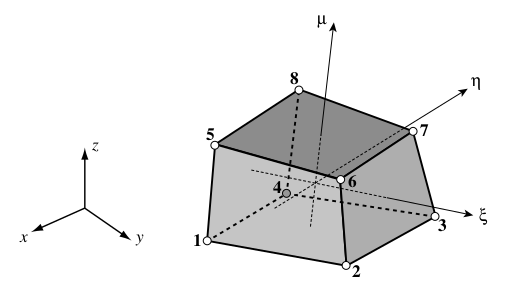
\includegraphics[width=0.90\textwidth]{img/hex8-node-numbers.png}
    \caption{The 8-node hexahedron and the natural coordinates $ \eta $, $ \xi $
    and $ \mu $.}
    \label{fig:hex8-node-numbers-png}
\end{figure}


\subsubsection{Element Definition}

The 8-noded hexahedral element is defined by:

\begin{eqarray}
    \begin{bmatrix}
        1\\
        x\\
        y\\
        z\\
        u_x\\
        u_y\\
        u_z
    \end{bmatrix} &=
    \begin{bmatrix}
        1 & 1 & 1 & 1 & 1 & 1 & 1 & 1\\
        x_1 & x_2 & x_3 & x_4 & x_5 & x_6 & x_7 & x_8\\
        y_1 & y_2 & y_3 & y_4 & y_5 & y_6 & y_7 & y_8\\
        y_1 & y_2 & y_3 & y_4 & y_5 & y_6 & y_7 & y_8\\
        u_{x1} & u_{x2} & u_{x3} & u_{x4} & u_{x5} & u_{x6} & u_{x7} & u_{x8}\\
        u_{y1} & u_{y2} & u_{y3} & u_{y4} & u_{y5} & u_{y6} & u_{y7} & u_{y8}\\
        u_{z1} & u_{z2} & u_{z3} & u_{z4} & u_{z5} & u_{z6} & u_{z7} & u_{z8}
    \end{bmatrix}
    \begin{bmatrix}
        N_1^e\\
        N_2^e\\
        N_3^e\\
        N_4^e\\
        N_5^e\\
        N_6^e\\
        N_7^e\\
        N_8^e
    \end{bmatrix}
\end{eqarray}

The hexahedron corners natural coordinates are:

\begin{table}[ht]
    \centering
    \begin{tabular}{|c c c c|}
        \hline
        node & $\xi$ & $\eta$ & $\mu$\\
        \hline
        1 & -1 & -1 & -1\\
        2 & +1 & -1 & -1\\
        3 & +1 & +1 & -1\\
        4 & -1 & +1 & -1\\
        5 & -1 & -1 & +1\\
        6 & +1 & -1 & +1\\
        7 & +1 & +1 & +1\\
        8 & -1 & +1 & +1\\
        \hline
    \end{tabular}\\
    \caption{Hexahedron corners natural coordinates}
\end{table}

The shape functions are:
\begin{eqarray}
    N_1^e &= \frac{1}{8} \left(1-\xi\right) \left(1-\eta\right) \left(1-\mu\right)\\
    N_2^e &= \frac{1}{8} \left(1+\xi\right) \left(1-\eta\right) \left(1-\mu\right)\\
    N_3^e &= \frac{1}{8} \left(1+\xi\right) \left(1+\eta\right) \left(1-\mu\right)\\
    N_4^e &= \frac{1}{8} \left(1-\xi\right) \left(1+\eta\right) \left(1-\mu\right)\\
    N_5^e &= \frac{1}{8} \left(1-\xi\right) \left(1-\eta\right) \left(1+\mu\right)\\
    N_6^e &= \frac{1}{8} \left(1+\xi\right) \left(1-\eta\right) \left(1+\mu\right)\\
    N_7^e &= \frac{1}{8} \left(1+\xi\right) \left(1+\eta\right) \left(1+\mu\right)\\
    N_8^e &= \frac{1}{8} \left(1-\xi\right) \left(1+\eta\right) \left(1+\mu\right)
\end{eqarray}

\begin{bbox}[0.96]
    The eight formulas can be summarised in a single expression:

    \begin{equation}
        N_i^e = \frac{1}{8}
              \left(1+\xi\xi_i\right)
              \left(1+\eta\eta_i\right)
              \left(1+\mu\mu_i\right)
    \end{equation}

    where $\xi_i$, $\eta_i$ and $\mu_i$ denote the coordinates of the $i$-th node.
\end{bbox}


\subsubsection{Partial Derivatives}
The calculation of the shape functions derivatives with respect to the natural
coordinates:

\begin{eqarray}
    \frac{\partial N_1^e}{\partial\xi} &= -\frac{1}{8} \left(1-\eta\right) \left(1-\mu\right)\\
    \frac{\partial N_2^e}{\partial\xi} &= \phantom{-}\frac{1}{8} \left(1-\eta\right) \left(1-\mu\right)\\
    \frac{\partial N_3^e}{\partial\xi} &= \phantom{-}\frac{1}{8} \left(1+\eta\right) \left(1-\mu\right)\\
    \frac{\partial N_4^e}{\partial\xi} &= -\frac{1}{8} \left(1+\eta\right) \left(1-\mu\right)\\
    \frac{\partial N_5^e}{\partial\xi} &= -\frac{1}{8} \left(1-\eta\right) \left(1+\mu\right)\\
    \frac{\partial N_6^e}{\partial\xi} &= \phantom{-}\frac{1}{8} \left(1-\eta\right) \left(1+\mu\right)\\
    \frac{\partial N_7^e}{\partial\xi} &= \phantom{-}\frac{1}{8} \left(1+\eta\right) \left(1+\mu\right)\\
    \frac{\partial N_8^e}{\partial\xi} &= -\frac{1}{8} \left(1+\eta\right) \left(1+\mu\right)
\end{eqarray}

\begin{eqarray}
    \frac{\partial N_1^e}{\partial\eta} &= -\frac{1}{8} \left(1-\xi\right) \left(1-\mu\right)\\
    \frac{\partial N_2^e}{\partial\eta} &= -\frac{1}{8} \left(1+\xi\right) \left(1-\mu\right)\\
    \frac{\partial N_3^e}{\partial\eta} &= \phantom{-}\frac{1}{8} \left(1+\xi\right) \left(1-\mu\right)\\
    \frac{\partial N_4^e}{\partial\eta} &= \phantom{-}\frac{1}{8} \left(1-\xi\right) \left(1-\mu\right)\\
    \frac{\partial N_5^e}{\partial\eta} &= -\frac{1}{8} \left(1-\xi\right) \left(1+\mu\right)\\
    \frac{\partial N_6^e}{\partial\eta} &= -\frac{1}{8} \left(1+\xi\right) \left(1+\mu\right)\\
    \frac{\partial N_7^e}{\partial\eta} &= \phantom{-}\frac{1}{8} \left(1+\xi\right) \left(1+\mu\right)\\
    \frac{\partial N_8^e}{\partial\eta} &= \phantom{-}\frac{1}{8} \left(1-\xi\right) \left(1+\mu\right)
\end{eqarray}

\begin{eqarray}
    \frac{\partial N_1^e}{\partial\mu} &= -\frac{1}{8} \left(1-\xi\right) \left(1-\eta\right)\\
    \frac{\partial N_2^e}{\partial\mu} &= -\frac{1}{8} \left(1+\xi\right) \left(1-\eta\right)\\
    \frac{\partial N_3^e}{\partial\mu} &= -\frac{1}{8} \left(1+\xi\right) \left(1+\eta\right)\\
    \frac{\partial N_4^e}{\partial\mu} &= -\frac{1}{8} \left(1-\xi\right) \left(1+\eta\right)\\
    \frac{\partial N_5^e}{\partial\mu} &= \phantom{-}\frac{1}{8} \left(1-\xi\right) \left(1-\eta\right)\\
    \frac{\partial N_6^e}{\partial\mu} &= \phantom{-}\frac{1}{8} \left(1+\xi\right) \left(1-\eta\right)\\
    \frac{\partial N_7^e}{\partial\mu} &= \phantom{-}\frac{1}{8} \left(1+\xi\right) \left(1+\eta\right)\\
    \frac{\partial N_8^e}{\partial\mu} &= \phantom{-}\frac{1}{8} \left(1-\xi\right) \left(1+\eta\right)
\end{eqarray}

\begin{bbox}
    \textbf{Note:}

    The partial derivatives can be also written as:

    \begin{eqarray}
        \frac{\partial N_i^e}{\partial \xi} &= \frac{1}{8} \frac{\xi_i}{|\xi_i|}
            \left(1+\eta\eta_i\right) \left(1+\mu\mu_i\right) \\
        \frac{\partial N_i^e}{\partial \eta} &= \frac{1}{8} \frac{\eta_i}{|\eta_i|}
            \left(1+\xi\xi_i\right) \left(1+\mu\mu_i\right) \\
        \frac{\partial N_i^e}{\partial \mu} &= \frac{1}{8} \frac{\mu_i}{|\mu_i|}
            \left(1+\xi\xi_i\right) \left(1+\eta\eta_i\right)
    \end{eqarray}
\end{bbox}



\textbf{The Jacobian:}

The derivatives of the shape functions are given by the usual chain rule formulas:

\begin{eqarray}
    \frac{\partial N_i^e}{\partial x} &=
        \frac{\partial N_i^e}{\partial \xi} \frac{\partial \xi}{\partial x} +
        \frac{\partial N_i^e}{\partial \eta} \frac{\partial \eta}{\partial x} +
        \frac{\partial N_i^e}{\partial \mu} \frac{\partial \mu}{\partial x}\\
    \frac{\partial N_i^e}{\partial y} &=
        \frac{\partial N_i^e}{\partial \xi} \frac{\partial \xi}{\partial y} +
        \frac{\partial N_i^e}{\partial \eta} \frac{\partial \eta}{\partial y} +
        \frac{\partial N_i^e}{\partial \mu} \frac{\partial \mu}{\partial y}\\
    \frac{\partial N_i^e}{\partial z} &=
        \frac{\partial N_i^e}{\partial \xi} \frac{\partial \xi}{\partial z} +
        \frac{\partial N_i^e}{\partial \eta} \frac{\partial \eta}{\partial z} +
        \frac{\partial N_i^e}{\partial \mu} \frac{\partial \mu}{\partial z}
\end{eqarray}

In matrix form:

\begin{eqarray}
    \begin{bmatrix}
        \frac{\partial N_i^e}{\partial x}\\
        \frac{\partial N_i^e}{\partial y}\\
        \frac{\partial N_i^e}{\partial z}
    \end{bmatrix} &=
    \begin{bmatrix}
        \frac{\partial \xi}{\partial x} &
        \frac{\partial \eta}{\partial x} &
        \frac{\partial \mu}{\partial x}\\
        \frac{\partial \xi}{\partial y} &
        \frac{\partial \eta}{\partial y} &
        \frac{\partial \mu}{\partial y}\\
        \frac{\partial \xi}{\partial z} &
        \frac{\partial \eta}{\partial z} &
        \frac{\partial \mu}{\partial z}
    \end{bmatrix}
    \begin{bmatrix}
        \frac{\partial N_i^e}{\partial \xi}\\
        \frac{\partial N_i^e}{\partial \eta}\\
        \frac{\partial N_i^e}{\partial \mu}
    \end{bmatrix}
\end{eqarray}

The $ 3 \times 3 $ matrix above is $ \m{J}^{-1} $, the inverse of:
\begin{eqarray}
    \m{J} = \frac{\partial \left( x, y, z \right)}{\partial \left( \xi, \eta, \mu \right)}
    = \begin{bmatrix}
        \frac{\partial x}{\partial \xi} &
        \frac{\partial y}{\partial \xi} &
        \frac{\partial z}{\partial \xi} \\
        \frac{\partial x}{\partial \eta} &
        \frac{\partial y}{\partial \eta} &
        \frac{\partial z}{\partial \eta} \\
        \frac{\partial x}{\partial \mu} &
        \frac{\partial y}{\partial \mu} &
        \frac{\partial z}{\partial \mu}
    \end{bmatrix}
\end{eqarray}

Matrix $ \m{J} $ is called the \textit{Jacobian matrix} of $ (x, y, z) $
with respect to $ (\xi, \eta, \mu) $. In the finite element literature, matrices
$ \m{J} $ and $ \m{J}^{-1} $ are called simply the \textit{Jacobian} and
\textit{inverse Jacobian}, respectively, although such a short name us sometimes
ambiguous. The notation

\begin{eqarray}
    \m{J} &=
    \frac{\partial \left(x, y, z \right)}{\partial \left(\xi, \eta, \mu \right)}\\
    \m{J}^{-1} &=
    \frac{\partial \left(\xi, \eta, \mu \right)}{\partial \left(x, y, z \right)}
\end{eqarray}

is standard in multivariable calculus and suggests that the Jacobian may be viewed as
a generalisation of the ordinary derivativem to which it reduces for a scalar
function $ \m{x} = x(\xi) $.



\subsubsection{Computing the Jacobian Matrix}
The isoparametric definitioin of hexahedron element geometry is:

\begin{eqarray}
    x &= x_i N_i^e\\
    y &= y_i N_i^e\\
    z &= z_i N_i^e
\end{eqarray}

where the summation convention is understood to apply over $ i = 1, 2, \dots , n $,
in which $ n $ denotes the number of element nodes.

\begin{bbox}
    \textbf{Note:} This for a given hexahedral element gives an $ n \times 3 $ matrix.
\end{bbox}


Differentiating these relations with respect to the hexahedron coordinates we construct
the matrix $ \m{J} $ as follows:

\begin{equation}
    \m{J} =
    \begin{bmatrix}
        x_i \frac{\partial N_i^e}{\partial \xi} &
        y_i \frac{\partial N_i^e}{\partial \xi} &
        z_i \frac{\partial N_i^e}{\partial \xi}\\
        x_i \frac{\partial N_i^e}{\partial \eta} &
        y_i \frac{\partial N_i^e}{\partial \eta} &
        z_i \frac{\partial N_i^e}{\partial \eta}\\
        x_i \frac{\partial N_i^e}{\partial \mu} &
        y_i \frac{\partial N_i^e}{\partial \mu} &
        z_i \frac{\partial N_i^e}{\partial \mu}
    \end{bmatrix}
\end{equation}

or:
\begin{equation}
    \m{J}_i =
    \begin{bmatrix}
        \frac{\partial N_1^e}{\partial \xi} &
        \frac{\partial N_2^e}{\partial \xi} &
        \dots &
        \frac{\partial N_n^e}{\partial \xi}\\
        \frac{\partial N_1^e}{\partial \eta} &
        \frac{\partial N_2^e}{\partial \eta} &
        \dots &
        \frac{\partial N_n^e}{\partial \eta}\\
        \frac{\partial N_1^e}{\partial \mu} &
        \frac{\partial N_2^e}{\partial \mu} &
        \dots &
        \frac{\partial N_n^e}{\partial \mu}
    \end{bmatrix}
    \begin{bmatrix}
        x_1 & y_1 & z_1 \\
        x_2 & y_2 & z_2 \\
        \vdots & \vdots & \vdots \\
        x_n & y_n & z_n
    \end{bmatrix}
\end{equation}


Given a point of hexahedron coordinates $ ( \xi, \eta, \mu ) $ the Jacobian $ \m{J} $
can be easilly formed using the above formula, and numerically inverted to form
$ \m{J}^{-1} $.


\subsubsection{The Strain-Displacement Matrix}

Having obtained the shape function derivatives, the matrix $ \m{B} $ for hexahedron
element displays the usual structure for 3D elements:

\begin{equation}
    \m{B} = \m{D}\m{\Phi} =
    \begin{bmatrix}
        \frac{\partial}{\partial x} & 0 & 0 \\
        0 & \frac{\partial}{\partial y} & 0 \\
        0 & 0 & \frac{\partial}{\partial z} \\
        \frac{\partial}{\partial y} & \frac{\partial}{\partial x} & 0 \\
        0 & \frac{\partial}{\partial z} & \frac{\partial}{\partial y} \\
        \frac{\partial}{\partial z} & 0 & \frac{\partial}{\partial x}
    \end{bmatrix}
    \begin{bmatrix}
        \m{q} & \m{0} & \m{0} \\
        \m{0} & \m{q} & \m{0} \\
        \m{0} & \m{0} & \m{q}
    \end{bmatrix} =
    \begin{bmatrix}
        \m{q}_x & \m{0} & \m{0} \\
        \m{0} & \m{q}_y & \m{0} \\
        \m{0} & \m{0} & \m{q}_z \\
        \m{q}_y & \m{q}_x & \m{0} \\
        \m{0} & \m{q}_z & \m{q}_y \\
        \m{q}_z & \m{0} & \m{q}_x
    \end{bmatrix}
\end{equation}

where:
\begin{eqarray}
    \m{q} &= \begin{bmatrix} N_1^e & \dots & N_n^e \end{bmatrix}\\
    \m{q}_x &= \begin{bmatrix} \frac{\partial N_1^e}{\partial x} & \dots & \frac{\partial N_n^e}{\partial x} \end{bmatrix}\\
    \m{q}_y &= \begin{bmatrix} \frac{\partial N_1^e}{\partial y} & \dots & \frac{\partial N_n^e}{\partial y} \end{bmatrix}\\
    \m{q}_z &= \begin{bmatrix} \frac{\partial N_1^e}{\partial z} & \dots & \frac{\partial N_n^e}{\partial z} \end{bmatrix}
\end{eqarray}

are row vectors of length $ n $, $ n $ being the number of nodes in the element.



\subsubsection{Stiffness Matrix Evaluation}

The element stiffness Matrix is given by:

\begin{equation}
    \m{K}^e = \int_{V^e} \m{B}^T \m{E} \m{B} dV^e
\end{equation}

As in two-dimensional case, this is replaced by a numerical integration formula which
now involves a triple loop over conventional Gauss quadrature rules. Assuming that
the stress-strain matrix $ \m{E} $ is constant over the element,

\begin{equation}
    \m{K}^e = \sum_{i=1}^{p_1} \sum_{j=1}^{p_2} \sum_{k=1}^{p_3}
    w_i w_j w_k \m{B}_{ijk}^T \m{E} \m{B}_{ijk} \m{J}_{ijk}
\end{equation}

Here $ p_1 $, $ p_2 $ and $ p_3 $ are the number of Gauss points in the $ \xi $,
$ \eta $ and $ \mu $ direction, respectively, while $ \m{B}_{ijk} $
and $ \m{J}_{ijk} $ are abbreviations for:

\begin{eqarray}
    \m{B}_{ijk} &= \m{B} \left(\xi_i, \eta_i, \mu_i\right) \\
    \m{J}_{ijk} &= det \m{J} \left(\xi_i, \eta_i, \mu_i\right)
\end{eqarray}

Usually the number of integration points is taken the same in all directions:
$ p = p_1 = p_2 = p_3 $. The total number of Gauss points is thus $ p^3 $.
Each point adds at most 6 to the stiffness matrix rank. The minimum rank-sufficient
rules for the 8-node and 20-node hexahedra are $ p = 2 $ and $ p = 3 $, respectively.


\subsection{Python implementation}

\begin{python}
#!/usr/bin/python3

import numpy as np
np.set_printoptions(precision=2) # , suppress=True)

def hex8_stiffness_mass_load(coors: np.ndarray,
                             E: float,
                             nu: float,
                             rho: float,
                             fx: float = 0.,
                             fy: float = 0.,
                             fz: float = 0.):
    """
    In:
        coors - 8 x 3 coordinate matrix
                [[x1,y1,z1], ... , [xn,yn,zn]
        E     - Youngs's Modulus
        nu    - Poisson's Constant
        rho   - Density
        fx    - Volumetric Load in x direction
        fy    - Volumetric Load in y direction
        fz    - Volumetric Load in z direction
    """
    domain = np.array([[-1., -1., -1.],
                       [1., -1., -1.],
                       [1., 1., -1.],
                       [-1., 1., -1.],
                       [-1., -1., 1.],
                       [1., -1., 1.],
                       [1., 1., 1.],
                       [-1., 1., 1.]], dtype=float)
    print('Domain: {0}\n{1}'.format(domain.shape, domain))

    # gaussian interpolation
    gauss_points = 3
    g_points, g_weights = np.polynomial.legendre.leggauss(gauss_points)
    integration_points = []
    interpolation_weights = []
    for i, xi in enumerate(g_points):
        for j, eta in enumerate(g_points):
            for k, mu in enumerate(g_points):
                integration_points.append([xi, eta, mu])
                interpolation_weights.append(g_weights[i] *
                                             g_weights[j] *
                                             g_weights[k])
    integration_points = np.array(integration_points, dtype=float)
    interpolation_weights = np.array(interpolation_weights, dtype=float)
    print('Gauss Integration '
          '{0}:\n{1}\nWeights:\n{2}'.format(gauss_points,
                                            integration_points,
                                            interpolation_weights))

    full_domain = np.vstack((domain, integration_points))

    # Shape Functions in Natural Coordinates
    xi = integration_points.T[0]
    eta = integration_points.T[1]
    mu = integration_points.T[2]
    psi = np.zeros((8, integration_points.shape[0]), dtype=float)
    for i in range(8):
        psi[i] = 1/8 * (1 + xi * domain[i, 0]) *
                       (1 + eta * domain[i, 1]) *
                       (1 + mu * domain[i, 2])
    psi = psi.T
    print('Shape Functions: {0}\n{1}'.format(psi.shape, psi))

    # Shape Functions in Global Coordinates
    psi_g = psi @ coors
    print('Shape Functions in '
          'Global Coordinates: {0}\n{1}'.format(psi_g.shape, psi_g))

    # Shape Functions Derivatives in Natural Coordinates
    dpsi = 1 / 8 * np.array([[(eta - 1.0) * (1.0 - mu),# 1
                              (xi - 1) * (1 - mu),
                             -(1 - xi) * (1 - eta)],
                             [(1 - eta) * (1 - mu),    # 2
                              (-1 - xi) * (1 - mu),
                             -(1 + xi) * (1 - eta)],
                             [(1 + eta) * (1 - mu),    # 3
                              (1 + xi) * (1 - mu),
                             -(1 + xi) * (1 + eta)],
                             [(-1.0 - eta) * (1 - mu), # 4
                              (1 - xi) * (1 - mu),
                             -(1 - xi) * (1 + eta)],
                             [(1 - eta) * (-1 - mu),   # 5
                             -(1 - xi) * (1 + mu),
                              (1 - xi) * (1 - eta)],
                             [(1 - eta) * (1 + mu),    # 6
                             -(1 + xi) * (1 + mu),
                              (1 + xi) * (1 - eta)],
                             [(1 + eta) * (1 + mu),    # 7
                              (1 + xi) * (1 + mu),
                              (1 + xi) * (1 + eta)],
                             [-(1 + eta) * (1 + mu),   # 8
                              (1 - xi) * (1 + mu),
                              (1 - xi) * (1 + eta)]])
    dpsi = dpsi.T
    print('Shape Functions Derivatives: '
          '{0}\n{1}'.format(dpsi.shape, dpsi))

    # Jacobian Matrix
    jacobi = dpsi @ coors
    print('Jacobian Matrix: {0}\n{1}'.format(jacobi.shape, jacobi))

    # Jacobian Determinants
    d_jacobi = np.linalg.det(jacobi)
    print('Determinant of Jacobian: '
          '{0}\n{1}'.format(d_jacobi.shape, d_jacobi))

    # Inverse Jacobian
    i_jacobi = np.linalg.inv(jacobi)
    print('Inverse Jacobian Matrix: '
          '{0}\n{1}'.format(i_jacobi.shape, i_jacobi))

    # Shape Function Derivatives in Global Coordinates
    dpsi_g = i_jacobi @ dpsi
    print('Shape Function Derivatives in Global Coordinates: '
          '{0}\n{1}'.format(dpsi_g.shape, dpsi_g))

    # Material Stiffness Matrix
    C = E / ((1.0 + nu) * (1.0 - 2.0 * nu)) *
        np.array([[1.0 - nu, nu, nu, 0.0, 0.0, 0.0],
                  [nu, 1.0 - nu, nu, 0.0, 0.0, 0.0],
                  [nu, nu, 1.0 - nu, 0.0, 0.0, 0.0],
                  [0.0, 0.0, 0.0, (1.0 - 2.0 * nu) / 2.0, 0.0, 0.0],
                  [0.0, 0.0, 0.0, 0.0, (1.0 - 2.0 * nu) / 2.0, 0.0],
                  [0.0, 0.0, 0.0, 0.0, 0.0, (1.0 - 2.0 * nu) / 2.0]],
                  dtype=float)
    print('Material Stiffness Matrix: {0}\n{1}'.format(C.shape, C))

    # Create Element Stiffness and Mass Matrix
    Ke = np.zeros((domain.size, domain.size), dtype=float)
    Me = np.zeros((domain.size, domain.size), dtype=float)
    Fe = np.zeros((domain.size, 1), dtype=float)
    # o = np.zeros(domain.shape[0], dtype=float)

    # iterate over Gauss points of domain, * means unpack values
    for i in range(integration_points.shape[0]):
        # this is smart but arranges dofs by component, not by node
        # component-wise dof ordering (x1, .. , y1, .. y4, z1, .. , z4)
        # B = np.array([
        #   [*dpsi_g[i, 0, :], *o, *o],
        #   [*o, *dpsi_g[i, 1, :], *o],
        #   [*o, *o, *dpsi_g[i, 2, :]],
        #   [*dpsi_g[i, 2, :], *o, *dpsi_g[i, 0, :]],
        #   [*o, *dpsi_g[i, 2, :], *dpsi_g[i, 1, :]],
        #   [*dpsi_g[i, 1, :], *dpsi_g[i, 0, :], *o]], dtype=float)

        # dofs ordered by node
        # node wise dof ordering (x1, y1, z1, .. , x4, y4, z4)
        dpx = dpsi_g[i,0,:]
        dpy = dpsi_g[i,1,:]
        dpz = dpsi_g[i,2,:]
        B = np.array(
            [[dpx[0],0,0,dpx[1],0,0,dpx[2],0,0,dpx[3],0,0],
             [0,dpy[0],0,0,dpy[1],0,0,dpy[2],0,0,dpy[3],0],
             [0,0,dpz[0],0,0,dpz[1],0,0,dpz[2],0,0,dpz[3]],
             [dpy[0],dpx[0],0,dpy[1],dpx[1],0,dpy[2],dpx[2],0,dpy[3],dpx[3],0],
             [0,dpz[0],dpy[0],0,dpz[1],dpy[1],0,dpz[2],dpy[2],0,dpz[3],dpy[3]],
             [dpz[0],0,dpx[0],dpz[1],0,dpx[1],dpz[2],0,dpx[2],dpz[3],0,dpx[3]],
             dtype=float)

        # component-wise dof ordering (x1, .. , y1, .. y4, z1, .. , z4)
        # N = np.array([[*psi[i], *o, *o],
        #               [*o, *psi[i], *o],
        #               [*o, *o, *psi[i]]], dtype=float)

        # node wise dof ordering (x1, y1, z1, .. , x4, y4, z4)
        N = np.array([[psi[i,0],0,0,psi[i,1],0,0,psi[i,2],0,0,psi[i,3],0,0],
                      [0,psi[i,0],0,0,psi[i,1],0,0,psi[i,2],0,0,psi[i,3],0],
                      [0,0,psi[i,0],0,0,psi[i,1],0,0,psi[i,2],0,0,psi[i,3]],
                      dtype=float)

        F = np.array([[fx], [fy], [fz]], dtype=float)

        Ke += (B.T @ C @ B) * d_jacobi[i] * interpolation_weights[i]
        Me += rho * (N.T @ N) * d_jacobi[i] * interpolation_weights[i]
        Fe += (N.T @ F) * d_jacobi[i] * interpolation_weights[i]

    print('Element Stiffness Matrix: {0}\n{1}'.format(Ke.shape, Ke))
    print('Element Mass Matrix: {0}\n{1}'.format(Me.shape, Me))
    print('Element Volume Force Vector: {0}\n{1}'.format(Fe.shape, Fe))
\end{python}

And to get stresses:
\begin{python}
#!/usr/bin/python3

import numpy as np
np.set_printoptions(precision=2) # , suppress=True)

def hex8_stresses(coors: np.ndarray,
                  disp: np.ndarray,
                  E: float,
                  nu: float):
    """
    In:
        coors - 8 x 3 coordinate matrix
                [[x1,y1,z1], ... , [xn,yn,zn]
        disp  - 8 x 3 coordinate matrix
                [[u1,v1,w1], ... , [un,vn,wn]
        E     - Youngs's Modulus
        nu    - Poisson's Constant
    """
    domain = np.array([[-1., -1., -1.],
                       [1., -1., -1.],
                       [1., 1., -1.],
                       [-1., 1., -1.],
                       [-1., -1., 1.],
                       [1., -1., 1.],
                       [1., 1., 1.],
                       [-1., 1., 1.]], dtype=float)
    print('Domain: {0}\n{1}'.format(domain.shape, domain))

    # gaussian interpolation
    gauss_points = 3
    g_points, g_weights = np.polynomial.legendre.leggauss(gauss_points)
    integration_points = []
    interpolation_weights = []
    for i, xi in enumerate(g_points):
        for j, eta in enumerate(g_points):
            for k, mu in enumerate(g_points):
                integration_points.append([xi, eta, mu])
                interpolation_weights.append(g_weights[i] *
                                             g_weights[j] *
                                             g_weights[k])
    integration_points = np.array(integration_points, dtype=float)
    interpolation_weights = np.array(interpolation_weights, dtype=float)
    print('Gauss Integration '
          '{0}:\n{1}\nWeights:\n{2}'.format(gauss_points,
                                            integration_points,
                                            interpolation_weights))

    full_domain = np.vstack((domain, integration_points))

    # Shape Functions in Natural Coordinates
    xi = integration_points.T[0]
    eta = integration_points.T[1]
    mu = integration_points.T[2]
    psi = np.zeros((8, integration_points.shape[0]), dtype=float)
    for i in range(8):
        psi[i] = 1/8 * (1 + xi * domain[i, 0]) *
                       (1 + eta * domain[i, 1]) *
                       (1 + mu * domain[i, 2])
    psi = psi.T
    print('Shape Functions: {0}\n{1}'.format(psi.shape, psi))

    # Shape Functions in Global Coordinates
    psi_g = psi @ coors
    print('Shape Functions in '
          'Global Coordinates: {0}\n{1}'.format(psi_g.shape, psi_g))

    # Shape Functions Derivatives in Natural Coordinates
    dpsi = 1 / 8 * np.array([[(eta - 1.0) * (1.0 - mu),# 1
                              (xi - 1) * (1 - mu),
                             -(1 - xi) * (1 - eta)],
                             [(1 - eta) * (1 - mu),    # 2
                              (-1 - xi) * (1 - mu),
                             -(1 + xi) * (1 - eta)],
                             [(1 + eta) * (1 - mu),    # 3
                              (1 + xi) * (1 - mu),
                             -(1 + xi) * (1 + eta)],
                             [(-1.0 - eta) * (1 - mu), # 4
                              (1 - xi) * (1 - mu),
                             -(1 - xi) * (1 + eta)],
                             [(1 - eta) * (-1 - mu),   # 5
                             -(1 - xi) * (1 + mu),
                              (1 - xi) * (1 - eta)],
                             [(1 - eta) * (1 + mu),    # 6
                             -(1 + xi) * (1 + mu),
                              (1 + xi) * (1 - eta)],
                             [(1 + eta) * (1 + mu),    # 7
                              (1 + xi) * (1 + mu),
                              (1 + xi) * (1 + eta)],
                             [-(1 + eta) * (1 + mu),   # 8
                              (1 - xi) * (1 + mu),
                              (1 - xi) * (1 + eta)]])
    dpsi = dpsi.T
    print('Shape Functions Derivatives: '
          '{0}\n{1}'.format(dpsi.shape, dpsi))

    # Jacobian Matrix
    jacobi = dpsi @ coors
    print('Jacobian Matrix: {0}\n{1}'.format(jacobi.shape, jacobi))

    # Jacobian Determinants
    d_jacobi = np.linalg.det(jacobi)
    print('Determinant of Jacobian: '
          '{0}\n{1}'.format(d_jacobi.shape, d_jacobi))

    # Inverse Jacobian
    i_jacobi = np.linalg.inv(jacobi)
    print('Inverse Jacobian Matrix: '
          '{0}\n{1}'.format(i_jacobi.shape, i_jacobi))

    # Shape Function Derivatives in Global Coordinates
    dpsi_g = i_jacobi @ dpsi
    print('Shape Function Derivatives in Global Coordinates: '
          '{0}\n{1}'.format(dpsi_g.shape, dpsi_g))

    # Material Stiffness Matrix
    C = E / ((1.0 + nu) * (1.0 - 2.0 * nu)) *
        np.array([[1.0 - nu, nu, nu, 0.0, 0.0, 0.0],
                  [nu, 1.0 - nu, nu, 0.0, 0.0, 0.0],
                  [nu, nu, 1.0 - nu, 0.0, 0.0, 0.0],
                  [0.0, 0.0, 0.0, (1.0 - 2.0 * nu) / 2.0, 0.0, 0.0],
                  [0.0, 0.0, 0.0, 0.0, (1.0 - 2.0 * nu) / 2.0, 0.0],
                  [0.0, 0.0, 0.0, 0.0, 0.0, (1.0 - 2.0 * nu) / 2.0]],
                  dtype=float)
    print('Material Stiffness Matrix: {0}\n{1}'.format(C.shape, C))

    du = disp.T @ np.transpose(dpsi_g, axes=[0, 2, 1])

    exx = du[:, 0, 0]
    eyy = du[:, 1, 1]
    ezz = du[:, 2, 2]
    exy = du[:, 0, 1] + du[:, 1, 0]
    eyz = du[:, 1, 2] + du[:, 2, 1]
    exz = du[:, 0, 2] + du[:, 2, 0]
    epsilons = np.array([exx, eyy, ezz, exy, eyz, exz])

    sigmas = (C @ epsilons).T
    epsilons = epsilons.T
    print('Element Strains: {0}\n{1}'.format(epsilons.shape, epsilons))
    print('Element Stresses: {0}\n{1}'.format(stresses.shape, stresses))
\end{python}




\newpage
\section{TET4 Element}

\subsection{Element Formulation}
For a linear tetrahedron no numerical integration is needed (there can be only
one integration point, shape functions derivatives are equal to 1).

The linear tetrahedron is not often used for stress analysis because of its poor
performance. Its main value in structural and solid mechanics is educational:
it serves as a vehicle to introduce the basic steps of formulation of 3D solid elements,
particularly with regards to the use of natural coordinate systems and node numbering
conventions. It should be noted that 3D visualisation is notoriously more difficult
than 2D, so it is needed to procede more slowly here.

\begin{figure}[ht]
    \centering
    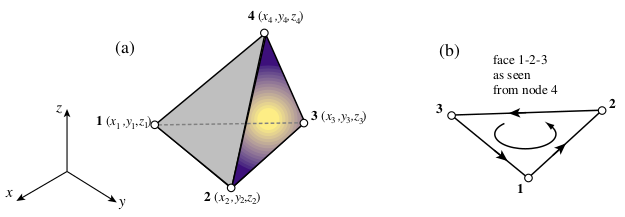
\includegraphics[width=0.90\textwidth]{img/linear_tetrahedron.png}
    \caption{(a)The linear tetrahedron element TET4, (b) Node numbering convention.}
    \label{fig:linear-tetrahedron-png}
\end{figure}


\subsubsection{Tetrahedron Geometry}

The tetrahedron geometry is fully defined by giving the location of the four
corner nodes with respect to Right-Hand Coordinate Sysetm notation $ (x, y, z) $:




\subsection{Python Implementation}
\begin{python}
#!/usr/bin/python3

import numpy as np
np.set_printoptions(precision=2) # , suppress=True)

def tet4_stiffness_mass_load(coors: np.ndarray,
                             E: float,
                             nu: float,
                             rho: float,
                             fx: float = 0.,
                             fy: float = 0.,
                             fz: float = 0.,
                             gauss_points = 4):
    domain = np.array([[1., 0., 0., 0.],
                       [0., 1., 0., 0.],
                       [0., 0., 1., 0.],
                       [0., 0., 0., 1.]], dtype=float)
    print('Domain: {0}\n{1}'.format(domain.shape, domain))

    # gaussian interpolation
    integration_points = None
    integration_weights = None
    if gauss_points == 1:
        integration_points = np.array([1/4, 1/4, 1/4, 1/4],
                                      dtype=float).reshape(1, 4)
        integration_weights = np.array([1 * 1 * 1 * 1],
                                       dtype=float) * 1/6

    elif gauss_points == 4:
        a = 0.58541020
        b = 0.13819660
        integration_points = np.array([[a, b, b, b],
                                       [b, a, b, b],
                                       [b, b, a, b],
                                       [b, b, b, a]], dtype=float)
        integration_weights = np.array([1/4, 1/4, 1/4, 1/4],
                                       dtype=float) * 1/6

    elif gauss_points == 5:
        integration_points = np.array([[1/4, 1/4, 1/4, 1/4],
                                       [1/2, 1/6, 1/6, 1/6],
                                       [1/6, 1/2, 1/6, 1/6],
                                       [1/6, 1/6, 1/2, 1/6],
                                       [1/6, 1/6, 1/6, 1/2]], dtype=float)
        integration_weights = np.array([-4/5, 9/20, 9/20, 9/20, 9/20],
                                       dtype=float) * 1/6

    print('Gauss Integration '
          '{0}:\n{1}\nWeights:\n{2}'.format(gauss_points,
                                            integration_points,
                                            integration_weights))

    full_domain = np.vstack((domain, integration_points))

    # Shape Functions in Natural Coordinates
    xi = integration_points.T[0]
    eta = integration_points.T[1]
    mu = integration_points.T[2]
    # zeta is not used to enforce
    # (1 - xi - eta - mu - zeta) = 0
    # zeta = integration_points.T[3]
    psi = np.zeros((4, integration_points.shape[0]), dtype=float)
    # another way of writing that psi = [xi, eta, mu, zeta]
    # for i in range(4):
    #     psi[i] = (1 + xi * domain[i, 0]) * (1 + eta * domain[i, 1]) * (1 + mu * domain[i, 2]) * (1 + zeta * domain[i, 3])
    psi[0] = xi
    psi[1] = eta
    psi[2] = mu
    psi[3] = 1 - xi - eta - mu  # = zeta
    psi = psi.T
    print('Shape Functions: {0}\n{1}'.format(psi.shape, psi))

    # Shape Functions in Global Coordinates
    psi_g = psi @ coors
    print('Shape Functions in Global Coordinates: '
          '{0}\n{1}'.format(psi_g.shape, psi_g))

    # Shape Functions Derivatives in Natural Coordinates
    dpsi = np.zeros((integration_points.shape[0], 4, 3), dtype=float)
    dpsi[:,0,0] = 1
    dpsi[:,1,1] = 1
    dpsi[:,2,2] = 1
    dpsi[:,3,:] = -1
    dpsi = dpsi.transpose((0, 2, 1))
    print('Shape Functions Derivatives: '
          '{0}\n{1}'.format(dpsi.shape, dpsi))

    # Jacobian Matrix
    jacobi = dpsi @ coors
    print('Jacobian Matrix: {0}\n{1}'.format(jacobi.shape, jacobi))

    # Jacobian Determinants
    d_jacobi = np.linalg.det(jacobi)
    print('Determinant of Jacobian: '
          '{0}\n{1}'.format(d_jacobi.shape, d_jacobi))

    # Inverse Jacobian
    i_jacobi = np.linalg.inv(jacobi)
    print('Inverse Jacobian Matrix: '
          '{0}\n{1}'.format(i_jacobi.shape, i_jacobi))

    # Shape Function Derivatives in Global Coordinates
    dpsi_g = i_jacobi @ dpsi
    print('Shape Function Derivatives in Global Coordinates: '
          '{0}\n{1}'.format(dpsi_g.shape, dpsi_g))

    # Material Stiffness Matrix
    C = E / ((1.0 + nu) * (1.0 - 2.0 * nu)) *
        np.array([[1.0 - nu, nu, nu, 0.0, 0.0, 0.0],
                  [nu, 1.0 - nu, nu, 0.0, 0.0, 0.0],
                  [nu, nu, 1.0 - nu, 0.0, 0.0, 0.0],
                  [0.0, 0.0, 0.0, (1.0 - 2.0 * nu) / 2.0, 0.0, 0.0],
                  [0.0, 0.0, 0.0, 0.0, (1.0 - 2.0 * nu) / 2.0, 0.0],
                  [0.0, 0.0, 0.0, 0.0, 0.0, (1.0 - 2.0 * nu) / 2.0]],
                  dtype=float)
    print('Material Stiffness Matrix: {0}\n{1}'.format(C.shape, C))

    # Create Element Stiffness and Mass Matrix
    Ke = np.zeros((domain.shape[0] * 3, domain.shape[0] * 3), dtype=float)
    Me = np.zeros((domain.shape[0] * 3, domain.shape[0] * 3), dtype=float)
    Fe = np.zeros((domain.shape[0] * 3, 1), dtype=float)
    o = np.zeros(domain.shape[0], dtype=float)

    # iterate over Gauss points of domain, * means unpack values
    for i in range(integration_points.shape[0]):
        # component-wise dof ordering (x1, .. , y1, .. y4, z1, .. , z4)
        # B = np.array([[*dpsi_g[i, 0, :], *o, *o],
        #               [*o, *dpsi_g[i, 1, :], *o],
        #               [*o, *o, *dpsi_g[i, 2, :]],
        #               [*dpsi_g[i, 2, :], *o, *dpsi_g[i, 0, :]],
        #               [*o, *dpsi_g[i, 2, :], *dpsi_g[i, 1, :]],
        #               [*dpsi_g[i, 1, :], *dpsi_g[i, 0, :], *o]],
        #               dtype=float)

        # node wise dof ordering (x1, y1, z1, .. , x4, y4, z4)
        dpx = dpsi_g[i,0,:]
        dpy = dpsi_g[i,1,:]
        dpz = dpsi_g[i,2,:]
        B = np.array(
            [[dpx[0],0,0,dpx[1],0,0,dpx[2],0,0,dpx[3],0,0],
             [0,dpy[0],0,0,dpy[1],0,0,dpy[2],0,0,dpy[3],0],
             [0,0,dpz[0],0,0,dpz[1],0,0,dpz[2],0,0,dpz[3]],
             [dpy[0],dpx[0],0,dpy[1],dpx[1],0,dpy[2],dpx[2],0,dpy[3],dpx[3],0],
             [0,dpz[0],dpy[0],0,dpz[1],dpy[1],0,dpz[2],dpy[2],0,dpz[3],dpy[3]],
             [dpz[0],0,dpx[0],dpz[1],0,dpx[1],dpz[2],0,dpx[2],dpz[3],0,dpx[3]],
             dtype=float)

        # component-wise dof ordering (x1, .. , y1, .. y4, z1, .. , z4)
        # N = np.array([[*psi[i], *o, *o],
        #               [*o, *psi[i], *o],
        #               [*o, *o, *psi[i]]], dtype=float)

        # node wise dof ordering (x1, y1, z1, .. , x4, y4, z4)
        N = np.array([[psi[i,0],0,0,psi[i,1],0,0,psi[i,2],0,0,psi[i,3],0,0],
                      [0,psi[i,0],0,0,psi[i,1],0,0,psi[i,2],0,0,psi[i,3],0],
                      [0,0,psi[i,0],0,0,psi[i,1],0,0,psi[i,2],0,0,psi[i,3]],
                      dtype=float)

        F = np.array([[fx], [fy], [fz]], dtype=float)

        print((B.T @ C @ B).shape)
        print(Ke.shape)
        Ke += (B.T @ C @ B) * d_jacobi[i] * integration_weights[i]
        Me += rho * (N.T @ N) * d_jacobi[i] * integration_weights[i]
        Fe += (N.T @ F) * d_jacobi[i] * integration_weights[i]

    print('Element Stiffness Matrix: {0}\n{1}'.format(Ke.shape, Ke))
    print('Element Mass Matrix: {0}\n{1}'.format(Me.shape, Me))
    print('Element Volume Force Vector: {0}\n{1}'.format(Fe.shape, Fe))
\end{python}


And to get stresses:
\begin{python}
#!/usr/bin/python3

import numpy as np
np.set_printoptions(precision=2) # , suppress=True)

def tet4_stresses(coors: np.ndarray,
                  disp: np.ndarray,
                  E: float,
                  nu: float):
    """
    In:
        coors - 4 x 3 coordinate matrix
                [[x1,y1,z1], ... , [xn,yn,zn]
        disp  - 4 x 3 coordinate matrix
                [[u1,v1,w1], ... , [un,vn,wn]
        E     - Youngs's Modulus
        nu    - Poisson's Constant
    """
    domain = np.array([[1., 0., 0., 0.],
                       [0., 1., 0., 0.],
                       [0., 0., 1., 0.],
                       [0., 0., 0., 1.]], dtype=float)
    print('Domain: {0}\n{1}'.format(domain.shape, domain))

    # gaussian interpolation
    integration_points = None
    integration_weights = None
    if gauss_points == 1:
        integration_points = np.array([1/4, 1/4, 1/4, 1/4],
                                      dtype=float).reshape(1, 4)
        integration_weights = np.array([1 * 1 * 1 * 1],
                                       dtype=float) * 1/6

    elif gauss_points == 4:
        a = 0.58541020
        b = 0.13819660
        integration_points = np.array([[a, b, b, b],
                                       [b, a, b, b],
                                       [b, b, a, b],
                                       [b, b, b, a]], dtype=float)
        integration_weights = np.array([1/4, 1/4, 1/4, 1/4],
                                       dtype=float) * 1/6

    elif gauss_points == 5:
        integration_points = np.array([[1/4, 1/4, 1/4, 1/4],
                                       [1/2, 1/6, 1/6, 1/6],
                                       [1/6, 1/2, 1/6, 1/6],
                                       [1/6, 1/6, 1/2, 1/6],
                                       [1/6, 1/6, 1/6, 1/2]], dtype=float)
        integration_weights = np.array([-4/5, 9/20, 9/20, 9/20, 9/20],
                                       dtype=float) * 1/6

    print('Gauss Integration '
          '{0}:\n{1}\nWeights:\n{2}'.format(gauss_points,
                                            integration_points,
                                            integration_weights))

    full_domain = np.vstack((domain, integration_points))

    # Shape Functions in Natural Coordinates
    xi = integration_points.T[0]
    eta = integration_points.T[1]
    mu = integration_points.T[2]
    # zeta is not used to enforce
    # (1 - xi - eta - mu - zeta) = 0
    # zeta = integration_points.T[3]
    psi = np.zeros((4, integration_points.shape[0]), dtype=float)
    # another way of writing that psi = [xi, eta, mu, zeta]
    # for i in range(4):
    #     psi[i] = (1 + xi * domain[i, 0]) * (1 + eta * domain[i, 1]) * (1 + mu * domain[i, 2]) * (1 + zeta * domain[i, 3])
    psi[0] = xi
    psi[1] = eta
    psi[2] = mu
    psi[3] = 1 - xi - eta - mu  # = zeta
    psi = psi.T
    print('Shape Functions: {0}\n{1}'.format(psi.shape, psi))

    # Shape Functions in Global Coordinates
    psi_g = psi @ coors
    print('Shape Functions in Global Coordinates: '
          '{0}\n{1}'.format(psi_g.shape, psi_g))

    # Shape Functions Derivatives in Natural Coordinates
    dpsi = np.zeros((integration_points.shape[0], 4, 3), dtype=float)
    dpsi[:,0,0] = 1
    dpsi[:,1,1] = 1
    dpsi[:,2,2] = 1
    dpsi[:,3,:] = -1
    dpsi = dpsi.transpose((0, 2, 1))
    print('Shape Functions Derivatives: '
          '{0}\n{1}'.format(dpsi.shape, dpsi))

    # Jacobian Matrix
    jacobi = dpsi @ coors
    print('Jacobian Matrix: {0}\n{1}'.format(jacobi.shape, jacobi))

    # Jacobian Determinants
    d_jacobi = np.linalg.det(jacobi)
    print('Determinant of Jacobian: '
          '{0}\n{1}'.format(d_jacobi.shape, d_jacobi))

    # Inverse Jacobian
    i_jacobi = np.linalg.inv(jacobi)
    print('Inverse Jacobian Matrix: '
          '{0}\n{1}'.format(i_jacobi.shape, i_jacobi))

    # Shape Function Derivatives in Global Coordinates
    dpsi_g = i_jacobi @ dpsi
    print('Shape Function Derivatives in Global Coordinates: '
          '{0}\n{1}'.format(dpsi_g.shape, dpsi_g))

    # Material Stiffness Matrix
    C = E / ((1.0 + nu) * (1.0 - 2.0 * nu)) *
        np.array([[1.0 - nu, nu, nu, 0.0, 0.0, 0.0],
                  [nu, 1.0 - nu, nu, 0.0, 0.0, 0.0],
                  [nu, nu, 1.0 - nu, 0.0, 0.0, 0.0],
                  [0.0, 0.0, 0.0, (1.0 - 2.0 * nu) / 2.0, 0.0, 0.0],
                  [0.0, 0.0, 0.0, 0.0, (1.0 - 2.0 * nu) / 2.0, 0.0],
                  [0.0, 0.0, 0.0, 0.0, 0.0, (1.0 - 2.0 * nu) / 2.0]],
                  dtype=float)
    print('Material Stiffness Matrix: {0}\n{1}'.format(C.shape, C))
    du = disp.T @ np.transpose(dpsi_g, axes=[0, 2, 1])

    exx = du[:, 0, 0]
    eyy = du[:, 1, 1]
    ezz = du[:, 2, 2]
    exy = du[:, 0, 1] + du[:, 1, 0]
    eyz = du[:, 1, 2] + du[:, 2, 1]
    exz = du[:, 0, 2] + du[:, 2, 0]
    epsilons = np.array([exx, eyy, ezz, exy, eyz, exz])

    sigmas = (C @ epsilons).T
    epsilons = epsilons.T
    print('Element Strains: {0}\n{1}'.format(epsilons.shape, epsilons))
    print('Element Stresses: {0}\n{1}'.format(stresses.shape, stresses))
\end{python}



\end{document}

